% Options for packages loaded elsewhere
\PassOptionsToPackage{unicode}{hyperref}
\PassOptionsToPackage{hyphens}{url}
%
\documentclass[
]{book}
\usepackage{lmodern}
\usepackage{amsmath}
\usepackage{ifxetex,ifluatex}
\ifnum 0\ifxetex 1\fi\ifluatex 1\fi=0 % if pdftex
  \usepackage[T1]{fontenc}
  \usepackage[utf8]{inputenc}
  \usepackage{textcomp} % provide euro and other symbols
  \usepackage{amssymb}
\else % if luatex or xetex
  \usepackage{unicode-math}
  \defaultfontfeatures{Scale=MatchLowercase}
  \defaultfontfeatures[\rmfamily]{Ligatures=TeX,Scale=1}
\fi
% Use upquote if available, for straight quotes in verbatim environments
\IfFileExists{upquote.sty}{\usepackage{upquote}}{}
\IfFileExists{microtype.sty}{% use microtype if available
  \usepackage[]{microtype}
  \UseMicrotypeSet[protrusion]{basicmath} % disable protrusion for tt fonts
}{}
\makeatletter
\@ifundefined{KOMAClassName}{% if non-KOMA class
  \IfFileExists{parskip.sty}{%
    \usepackage{parskip}
  }{% else
    \setlength{\parindent}{0pt}
    \setlength{\parskip}{6pt plus 2pt minus 1pt}}
}{% if KOMA class
  \KOMAoptions{parskip=half}}
\makeatother
\usepackage{xcolor}
\IfFileExists{xurl.sty}{\usepackage{xurl}}{} % add URL line breaks if available
\IfFileExists{bookmark.sty}{\usepackage{bookmark}}{\usepackage{hyperref}}
\hypersetup{
  pdftitle={Bioestadística: preguntas y problemas resueltos},
  pdfauthor={Javier Manzano},
  hidelinks,
  pdfcreator={LaTeX via pandoc}}
\urlstyle{same} % disable monospaced font for URLs
\usepackage{longtable,booktabs}
\usepackage{calc} % for calculating minipage widths
% Correct order of tables after \paragraph or \subparagraph
\usepackage{etoolbox}
\makeatletter
\patchcmd\longtable{\par}{\if@noskipsec\mbox{}\fi\par}{}{}
\makeatother
% Allow footnotes in longtable head/foot
\IfFileExists{footnotehyper.sty}{\usepackage{footnotehyper}}{\usepackage{footnote}}
\makesavenoteenv{longtable}
\usepackage{graphicx}
\makeatletter
\def\maxwidth{\ifdim\Gin@nat@width>\linewidth\linewidth\else\Gin@nat@width\fi}
\def\maxheight{\ifdim\Gin@nat@height>\textheight\textheight\else\Gin@nat@height\fi}
\makeatother
% Scale images if necessary, so that they will not overflow the page
% margins by default, and it is still possible to overwrite the defaults
% using explicit options in \includegraphics[width, height, ...]{}
\setkeys{Gin}{width=\maxwidth,height=\maxheight,keepaspectratio}
% Set default figure placement to htbp
\makeatletter
\def\fps@figure{htbp}
\makeatother
\setlength{\emergencystretch}{3em} % prevent overfull lines
\providecommand{\tightlist}{%
  \setlength{\itemsep}{0pt}\setlength{\parskip}{0pt}}
\setcounter{secnumdepth}{5}
\usepackage{booktabs}
\usepackage[spanish]{babel}
\decimalpoint
\selectlanguage{spanish}
\ifluatex
  \usepackage{selnolig}  % disable illegal ligatures
\fi
\usepackage[]{natbib}
\bibliographystyle{apalike}

\title{Bioestadística: preguntas y problemas resueltos}
\author{Javier Manzano}
\date{2023-10-13}

\begin{document}
\maketitle

{
\setcounter{tocdepth}{1}
\tableofcontents
}
\hypertarget{introducciuxf3n}{%
\chapter{Introducción}\label{introducciuxf3n}}

En estas páginas encontrarás preguntas tipo test y problemas de exámenes resueltos además de prácticas para la asignatura de Bioestadística en Grados de Ciencias de la Salud (Enfermería, Fisioterapia, Farmacia, etc.) y de exámenes BIR/FIR/QIR con las explicaciones correspondientes.

Para un eficaz, efectivo y eficiente uso del contenido de estas páginas, se recomienda el uso de \emph{papel y bolígrafo}.

Estas páginas son un complemento del \href{https://1fjmanzano.github.io/bioestadistica/}{Curso de Bioestadística} que incluye prácticas con Excel©.

En temario sobre el que basamos esta colección de problemas es el de la asignatura de la Universidad de Salamanca que incluye los siguientes bloques temáticos:

\begin{itemize}
\item
  Planteamiento de una investigación: Anatomía y Fisiología de la investigación
\item
  Análisis Descriptivo y Gráfico de datos cuantitativos
\item
  Análisis Inferencial. Aplicaciones.
\item
  Regresión y correlación.
\item
  Tablas de contingencia.
\item
  Medidas de importancia clínica.
\end{itemize}

Después de cada pregunta tipo test hay un botón para ver la respuesta correcta así como un enlace a la Explicación correspondiente.

Respuesta correcta

Respuesta correcta

\hypertarget{planteamiento-de-una-investigaciuxf3n-anatomuxeda-y-fisiologuxeda-de-la-investigaciuxf3n}{%
\chapter{Planteamiento de una investigación: Anatomía y Fisiología de la investigación}\label{planteamiento-de-una-investigaciuxf3n-anatomuxeda-y-fisiologuxeda-de-la-investigaciuxf3n}}

En este capítulo se resolverán problemas relativos a:

\begin{itemize}
\tightlist
\item
  Diseño de una investigación
\item
  Métodos de muestreo
\item
  Métodos de recolección de datos
\item
  Variables y Escalas de Medida
\item
  Errores en la Investigación
\end{itemize}

\hypertarget{pregunta-test}{%
\section{Pregunta test}\label{pregunta-test}}

La proporción de individuos de una población que tiene una enfermedad en un momento dado de tiempo se denomina:

\begin{enumerate}
\def\labelenumi{\alph{enumi})}
\tightlist
\item
  Incidencia acumulada
\item
  Densidad de incidencia
\item
  Fracción atribuible
\item
  Prevalencia
\item
  Odds ratio
\end{enumerate}

Respuesta correcta

\href{https://www.cancer.gov/espanol/publicaciones/diccionarios/diccionario-cancer/def/prevalencia}{Explicación}

\hypertarget{pregunta-test-1}{%
\section{Pregunta test}\label{pregunta-test-1}}

Es una Variable Cualitativa Ordinal:

\begin{enumerate}
\def\labelenumi{\alph{enumi})}
\tightlist
\item
  Sexo (M, F).
\item
  Bebe (no, poco, mucho).
\item
  Nº de muelas cariadas.
\item
  Temperatura corporal.
\item
  Raza (blanca, negra, amarilla).
\end{enumerate}

Respuesta correcta

\href{https://1fjmanzano.github.io/bioestadistica/tipos-de-variables.html}{Explicación}

\hypertarget{pregunta-test-2}{%
\section{Pregunta test}\label{pregunta-test-2}}

¿Cuál es el mejor tipo de estudio epidemiológico para estimar la prevalencia de una enfermedad crónica en una comunidad determinada?

\begin{enumerate}
\def\labelenumi{\alph{enumi})}
\tightlist
\item
  Estudio ecológico
\item
  Ensayo clínico aleatorio
\item
  Estudio transversal de la población
\item
  Estudio de casos y controles
\item
  Estudio de cohortes
\end{enumerate}

Respuesta correcta

\href{https://escuelitamedica.com/2019/02/03/tipos-de-estudios-epidemiologicos-preguntas/}{Explicación}

\hypertarget{problema}{%
\section{Problema}\label{problema}}

\begin{enumerate}
\def\labelenumi{\arabic{enumi}.}
\tightlist
\item
  El Ministerio de Sanidad, Servicios Sociales e Igualdad ha publicado recientemente el Barómetro Sanitario nacional, correspondiente a 2011.
\end{enumerate}

\textbf{a)} Según los resultados del estudio, de los 7757 encuestados, 2487 afirman ser fumadores en la actualidad, 5262 afirman ser no fumadores y el resto no contesta. Construye la tabla de frecuencias correspondiente y realiza una gráfica representativa de la distribución de la muestra según el hábito de fumar.

\textbf{b)} A aquellos que habían declarado ser fumadores se les preguntó a continuación como habían influido en su consumo las medidas de la nueva Ley del tabaco. A continuación se muestra una tabla incompleta que resume las respuestas. Completa la tabla y realiza una gráfica representativa.

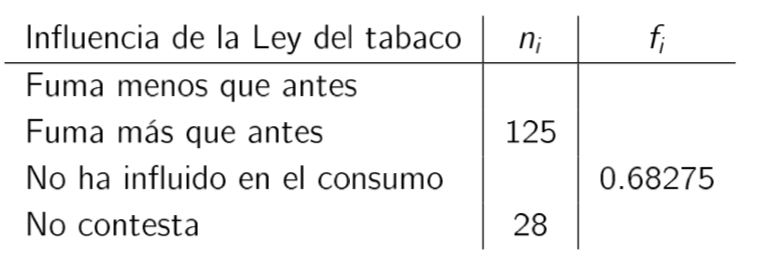
\includegraphics[width=10.58in]{img/1_01}

\hypertarget{soluciuxf3n}{%
\subsection{Solución}\label{soluciuxf3n}}

\textbf{a)} Construimos la tabla de frecuencias con Excel© según esta \href{https://1fjmanzano.github.io/bioestadistica/tablas-de-frecuencias.html\#tabla-de-frecuencias-pr\%C3\%A1ctica-con-excel}{Práctica del Curso de Bioestadística}:

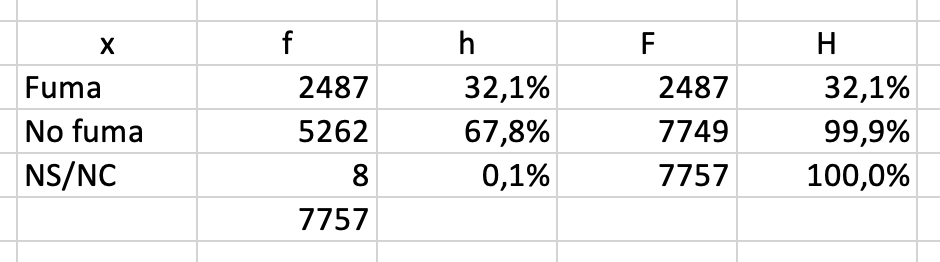
\includegraphics[width=13.06in]{img/1_02}

Con los datos de la tabla, hacemos un diagrama de sectores según esta \href{https://1fjmanzano.github.io/bioestadistica/diagramas-de-barras-y-sectores.html\#diagramas-de-barras-y-sectores-pr\%C3\%A1ctica-con-excel}{Práctica del Curso de Bioestadística}

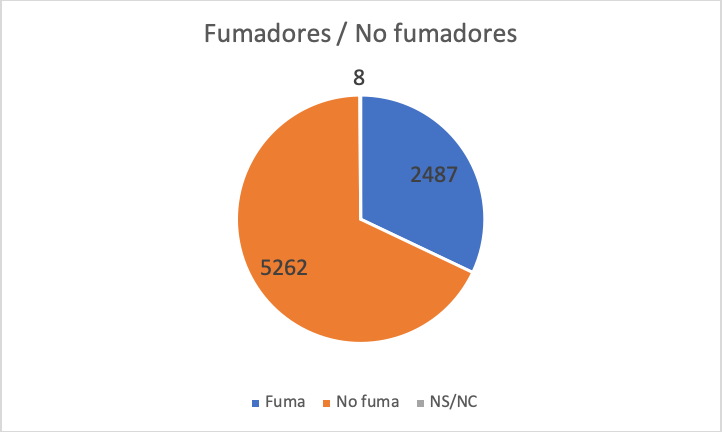
\includegraphics[width=10.03in]{img/1_03}

\textbf{b)} En este caso, se pregunta a los que habían declarado ser fumadores por lo que \(N = 2487\). Como la frecuencia relativa de la opción ``No ha influido en el consumo'' es \(0,68275\), la refuencia absoluta es \(0,68275 \cdot 2487 = 1697,99925 \approx 1698\) (no puede haber decimales). No tenemos más que calcular la frecuencia absoluta de la opción ``Fuma menos que antes'', \(2487 - 28 - 1698 - 125 = 636\) y completar la tabla con las frecuencias relativas:

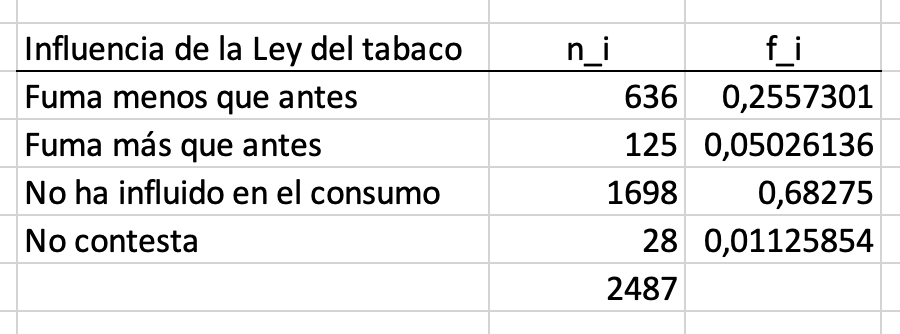
\includegraphics[width=12.5in]{img/1_04}

Finalmente, obtenemos un diagrama de barras de los datos:

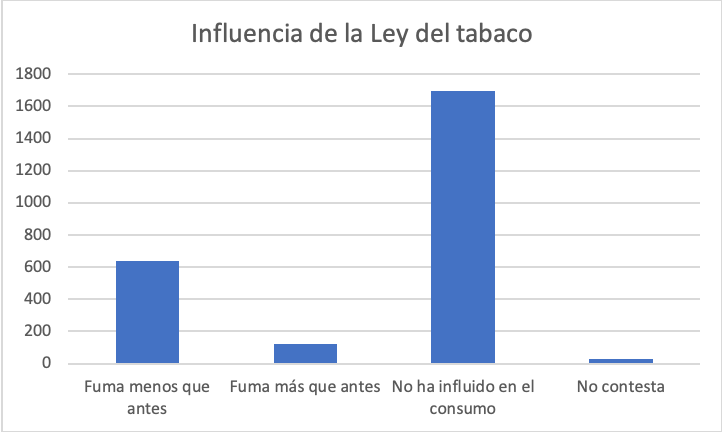
\includegraphics[width=10.03in]{img/1_05}

\hypertarget{pregunta-test-3}{%
\section{Pregunta test}\label{pregunta-test-3}}

Se realiza una auditoría de historias clínicas tomando una primera historia al azar y después sucesivamente, la que ocupa la vigésima posición detrás de la anterior. Este procedimiento de muestreo se denomina:

\begin{enumerate}
\def\labelenumi{\alph{enumi})}
\tightlist
\item
  Por conglomerados.
\item
  Sistemático.
\item
  Correlativo.
\item
  Consecutivo.
\item
  Equidistante.
\end{enumerate}

Respuesta correcta

\href{https://1fjmanzano.github.io/bioestadistica/me\%CC\%81todos-de-muestreo.html}{Explicación}

\hypertarget{pregunta-test-4}{%
\section{Pregunta test}\label{pregunta-test-4}}

En una muestra de pacientes, el número de varones dividido entre el total de pacientes es:

\begin{enumerate}
\def\labelenumi{\alph{enumi})}
\tightlist
\item
  Una frecuencia relativa.
\item
  Una frecuencia absoluta.
\item
  Una variable cuantitativa.
\item
  Una variable cualitativa.
\item
  Un valor de la variable.
\end{enumerate}

Respuesta correcta

\href{https://1fjmanzano.github.io/bioestadistica/tablas-de-frecuencias.html}{Explicación}

\hypertarget{pregunta-test-5}{%
\section{Pregunta test}\label{pregunta-test-5}}

Señale cuál de las siguientes afirmaciones es falsa:

\begin{enumerate}
\def\labelenumi{\alph{enumi})}
\tightlist
\item
  La aparición o no de bacterias en un cultivo es una variable dicotómica
\item
  La estatura de un individuo es una variable cuantitativa discreta.
\item
  El lugar que ocupa una persona entre sus hermanos (de menor a mayor edad) es una variable ordinal.
\item
  El estado civil es una variable cualitativa.
\item
  La glucemia es continua.
\end{enumerate}

Respuesta correcta

\href{https://1fjmanzano.github.io/bioestadistica/tipos-de-variables.html}{Explicación}

\hypertarget{problema-1}{%
\section{Problema}\label{problema-1}}

En base a la siguiente distribución de frecuencias relativas acumuladas de la variable \(X\) = ``Número de contratos conseguidos en el mes de enero'' obtenida de la observación de la actividad de 50 teleoperadores de
una compañía de telefonía móvil, indique el número mínimo de contratos que tiene que haber conseguido un teleoperador para estar entre los 5 que han destacado más:

\begin{longtable}[]{@{}cccccccc@{}}
\toprule
\(X_i\) & 58 & 60 & 62 & 65 & 68 & 70 & 71\tabularnewline
\midrule
\endhead
\(H_i\) & 0.06 & 0.2 & 0.4 & 0.64 & 0.8 & 0.92 & 1\tabularnewline
\bottomrule
\end{longtable}

\hypertarget{soluciuxf3n-1}{%
\subsection{Solución}\label{soluciuxf3n-1}}

Al haber 50 teleoperadores, si tiene que estar entre los 5 que han destacado mas, debe dejar a 45 por detrás. Como \(\frac{45}{50}=0.9\), deberá superar al 90 \%, es decir, estar por encima del 0.9 en la frecuencia relativa acumulada.

En la tabla vemos que para el valor 70 se alcanza la frecuencia relativa acumulada de 0.92 por lo que \textbf{para estar entre los 5 que más han destacado, deberá haber firmado, al menos, 70 contratos}.

\hypertarget{pregunta-test-6}{%
\section{Pregunta test}\label{pregunta-test-6}}

¿A qué fase del proceso de investigación pertenece la recogida, análisis e interpretación de los resultados?

\begin{enumerate}
\def\labelenumi{\alph{enumi})}
\tightlist
\item
  Fase conceptual.
\item
  Fase Metodológica.
\item
  Fase Empírica.
\item
  Fase de análisis e interpretación de los datos.
\end{enumerate}

Respuesta correcta

\href{https://www.salusplay.com/apuntes/apuntes-metodologia-de-la-investigacion/tema-4-el-proceso-de-investigacion-fases-de-realizacion-de-una-investigacion-cientifica/2}{Explicación}

\hypertarget{pregunta-test-7}{%
\section{Pregunta test}\label{pregunta-test-7}}

La incidencia de una enfermedad es:

\begin{enumerate}
\def\labelenumi{\alph{enumi})}
\tightlist
\item
  La relación entre enfermos y fallecidos
\item
  La prevalencia multiplicada por la morbilidad
\item
  Lo mismo que la prevalencia
\item
  El nº de casos nuevos de esa enfermedad
\item
  Ninguna de las anteriores
\end{enumerate}

Respuesta correcta

\href{https://medlineplus.gov/spanish/ency/article/002387.htm}{Explicación}

\hypertarget{pregunta-test-8}{%
\section{Pregunta test}\label{pregunta-test-8}}

En el caso de una variable ordinal, el número n de datos válidos es:

\begin{enumerate}
\def\labelenumi{\alph{enumi})}
\tightlist
\item
  La suma de las frecuencias absolutas.
\item
  La frecuencia absoluta acumulada de la categoría más frecuente.
\item
  La suma de las frecuencias relativas.
\item
  La frecuencia relativa acumulada en la última categoría.
\item
  La (a) y la (d) son ciertas.
\end{enumerate}

Respuesta correcta

\href{https://1fjmanzano.github.io/bioestadistica/tablas-de-frecuencias.html}{Explicación}

\hypertarget{pregunta-test-9}{%
\section{Pregunta test}\label{pregunta-test-9}}

El nº de casos nuevos de una enfermedad que se desarrolla en una población en un periodo de tiempo determinado se conoce como:

\begin{enumerate}
\def\labelenumi{\alph{enumi})}
\tightlist
\item
  Densidad de incidencia
\item
  Incidencia acumulada
\item
  Prevalencia
\item
  Fracción atribuible
\item
  Riesgo relativo
\end{enumerate}

Respuesta correcta

\href{https://www.conprueba.es/glosario/incidencia-acumulada}{Explicación}

\hypertarget{pregunta-test-10}{%
\section{Pregunta test}\label{pregunta-test-10}}

Se realiza un estudio con objeto de determinar el tiempo de supervivencia en pacientes con cáncer. Para ello de los dos hospitales existentes en una ciudad, se selecciona aleatoriamente uno de ellos, y se elige una muestra aleatoria de pacientes, atendiendo al tipo de cáncer: El muestreo realizado es:

\begin{enumerate}
\def\labelenumi{\alph{enumi})}
\tightlist
\item
  Sistemático.
\item
  Aleatorio.
\item
  Por conglomerados.
\item
  Estratificado.
\item
  Por conglomerados y estratificado.
\end{enumerate}

Respuesta correcta

\hypertarget{pregunta-test-11}{%
\section{Pregunta test}\label{pregunta-test-11}}

En un estudio sobre problemas cervicales preguntamos a los pacientes acerca del tipo de almohada que usan. Las respuestas deberían ser consideradas como una variable:

\begin{enumerate}
\def\labelenumi{\alph{enumi})}
\tightlist
\item
  Cualitativa nominal
\item
  Numérica
\item
  Discreta
\item
  Continua.
\item
  Ordinal
\end{enumerate}

Respuesta correcta

\href{https://1fjmanzano.github.io/bioestadistica/tipos-de-variables.html}{Explicación}

\hypertarget{pregunta-test-12}{%
\section{Pregunta test}\label{pregunta-test-12}}

Al inicio de un estudio de cohortes ¿cómo está la población a estudiar?

\begin{enumerate}
\def\labelenumi{\alph{enumi})}
\tightlist
\item
  Todos los efectos del proceso que se estudia
\item
  Todos sanos
\item
  La cohorte expuesta sana y la no expuesta enferma
\item
  La cohorte expuesta enferma y la no expuesta sana
\item
  Ninguna de las anteriores
\end{enumerate}

Respuesta correcta

\href{https://es.wikipedia.org/wiki/Estudio_de_cohorte}{Explicación}

\hypertarget{problema-2}{%
\section{Problema}\label{problema-2}}

De la distribución de la variable \(X\) = `Peso (en Kg)' de un colectivo de adolescentes agrupada en 4 intervalos con límites superiores 60, 65, 70 y 75 se sabe que:

\begin{itemize}
\tightlist
\item
  la mitad del colectivo pesa entre 65 y 70 kg
\item
  una cuarta parte pesa como máximo 65 kg
\item
  9 adolescentes tiene un peso máximo de 60 kg
\item
  18 pesan entre 70 y 75 kg.
\end{itemize}

Calcula

\textbf{a)} El número n de adolescentes entrevistados

\textbf{b)} El porcentaje de adolescentes que pesan entre 55 y 60 kg

\textbf{c)} El peso mínimo de la mitad de adolescentes con mayor peso

\textbf{d) } Cuántos alumnos pesan como máximo, 65 kg

\hypertarget{soluciuxf3n-2}{%
\subsection{Solución}\label{soluciuxf3n-2}}

Vemos que tenemos mucha información que conviene organizar en forma de tabla. Empezamos escribiendo una tabla con los datos que tenemos:

\begin{longtable}[]{@{}ccccc@{}}
\toprule
Intervalo & \(f_i\) & \(h_i\) & \(F_i\) & \(H_i\)\tabularnewline
\midrule
\endhead
\([55,60)\) & 9 & & 9 &\tabularnewline
\([60,65)\) & & & & 0.25\tabularnewline
\([65,70)\) & & 0.50 & &\tabularnewline
\([70,75)\) & 18 & & & 1\tabularnewline
\bottomrule
\end{longtable}

A partir de estos datos, vamos a completar el resto.

Como el 25 \% pesan menos de 65 y el 50 \% entre 65 y 70, entonces el 75 \% pesarán menos de 70 kg y el 25 \% pesarán más de 70 hg.

\begin{longtable}[]{@{}ccccc@{}}
\toprule
Intervalo & \(f_i\) & \(h_i\) & \(F_i\) & \(H_i\)\tabularnewline
\midrule
\endhead
\([55,60)\) & 9 & & 9 &\tabularnewline
\([60,65)\) & & & & 0.25\tabularnewline
\([65,70)\) & & 0.50 & & 0.75\tabularnewline
\([70,75)\) & 18 & 0.25 & & 1\tabularnewline
\bottomrule
\end{longtable}

Así, el 25 \% (la cuarta parte) del número n de adolescentes entrevistados es 18 por lo que \(n = 18 \cdot 4 = 72\). El 50 \% de 72 es 36 y, como hay 9 adolescentes entre 55 y 60 kg y como \(72 - 9 - 36 - 18 = 9\), tendremos

\begin{longtable}[]{@{}ccccc@{}}
\toprule
Intervalo & \(f_i\) & \(h_i\) & \(F_i\) & \(H_i\)\tabularnewline
\midrule
\endhead
\([55,60)\) & 9 & 0.125 & 9 & 0.125\tabularnewline
\([60,65)\) & 9 & 0.125 & 18 & 0.25\tabularnewline
\([65,70)\) & 36 & 0.50 & 54 & 0.75\tabularnewline
\([70,75)\) & 18 & 0.25 & 72 & 1\tabularnewline
\bottomrule
\end{longtable}

Y a la vista de la tabla, podemos responder a las preguntas:

\textbf{a)} Se entrevistaron a 72 adolescentes

\textbf{b)} El 25 \% de adolescentes pesa entre 55 y 60 kg

\textbf{c)} El 50 \% de los adolescentes con mayor peso están en los intervalos \([65,70)\) y \([70,75)\) y, como no podemos saber exactamente cuál es el peso menor de ese 50 \%, \textbf{el peso mínimo de la mitad de adolescentes con mayor peso es de, al menos, 65 kg}.

\textbf{d)} 18 alumnos pesan como máximo 65 kg

\hypertarget{pregunta-test-13}{%
\section{Pregunta test}\label{pregunta-test-13}}

¿Cuál de las siguientes características pertenece al paradigma naturalista?

\begin{enumerate}
\def\labelenumi{\alph{enumi})}
\tightlist
\item
  Pretende buscar la objetividad.
\item
  El investigador interactúa con los sujetos investigados y los resultados se crean de esa interacción.
\item
  Utilización de procesos deductivos.
\item
  Importancia en el análisis estadístico.
\end{enumerate}

Respuesta correcta

\href{https://www.encyclo.co.uk/meaning-of-Naturalistic_paradigm}{Explicación}

\hypertarget{pregunta-test-14}{%
\section{Pregunta test}\label{pregunta-test-14}}

En un estudio sobre la enfermedad coronaria en la población española, se selecciona una muestra de individuos hipertensos y un grupo de control de no hipertensos. Se les sigue durante 5 años y se compara la incidencia de la enfermedad de ambos grupos ¿A qué tipo de diseño corresponde el estudio?

\begin{enumerate}
\def\labelenumi{\alph{enumi})}
\tightlist
\item
  Estudio de cohortes
\item
  Estudio de casos y controles
\item
  Estudio transversal
\item
  Ensayo clínico
\item
  Estudio ecológico
\end{enumerate}

Respuesta correcta

\href{https://es.wikipedia.org/wiki/Estudio_de_cohorte}{Explicación}

\hypertarget{pregunta-test-15}{%
\section{Pregunta test}\label{pregunta-test-15}}

Se desea estimar confidencialmente el número medio de veces que asiste a un servicio de salud los individuos de una población. Para ello se toman muestras aleatorias entre los individuos que asisten regularmente a los mismos. Esta técnica de muestreo es:

\begin{enumerate}
\def\labelenumi{\alph{enumi})}
\tightlist
\item
  Un muestreo aleatorio simple.
\item
  Un muestreo aleatorio estratificado.
\item
  Un muestreo aleatorio por conglomerados.
\item
  Incorrecta.
\item
  Ninguna de las anteriores.
\end{enumerate}

Respuesta correcta

\hypertarget{pregunta-test-16}{%
\section{Pregunta test}\label{pregunta-test-16}}

El estudio estadístico en el que se pretenden extrapolar los datos de una muestra a la población se denomina:

\begin{enumerate}
\def\labelenumi{\alph{enumi})}
\tightlist
\item
  Estadística descriptiva.
\item
  Estadística inferencial.
\item
  Medidas de tendencia central.
\item
  Medidas de posición.
\end{enumerate}

Respuesta correcta

\href{https://1fjmanzano.github.io/bioestadistica/inferencia-estad\%C3\%ADstica.html}{Explicación}

\hypertarget{problema-3}{%
\section{Problema}\label{problema-3}}

Con el objetivo de programar las actividades en un consultorio se obtiene información del número de consultas realizadas el año anterior:

\begin{longtable}[]{@{}ccc@{}}
\toprule
& Mujeres & Hombres\tabularnewline
\midrule
\endhead
Intervalo & n & n\tabularnewline
1 - 3 & 18 & 22\tabularnewline
4 - 6 & 39 & 31\tabularnewline
7 - 9 & 53 & 46\tabularnewline
8 - 10 & 45 & 40\tabularnewline
11 - 13 & 53 & 35\tabularnewline
14 - 16 & 39 & 29\tabularnewline
17 - 20 & 18 & 26\tabularnewline
Total & 265 & 229\tabularnewline
\bottomrule
\end{longtable}

\textbf{a)} Indique el (o los) nombre(s) de las(s) variables(s) de la tabla e identifique sus categorías.

\textbf{b)} Indique el tipo de escala de las(s) variables (s) de la tabla.

\textbf{c)} ¿Qué porcentaje de pacientes realiza, al menos, 8 consultas?

\hypertarget{soluciuxf3n-3}{%
\subsection{Solución}\label{soluciuxf3n-3}}

\textbf{a)} La variable estudiada es \textbf{número de consultas realizadas el año anterior con 2 categorías, Mujeres y Hombres}.

\textbf{b)} Es una variable cualitativa discreta de escala ordinal con resultados agrupados en intervalos.

\textbf{c)} Para calcular el porcentaje pedido, vemos que:

\begin{itemize}
\item
  Mujeres con, al menos 8 consultas: \(45 + 53 + 39 + 18 = 155\)
\item
  Hombres con, al menos 8 consultas: \(40 + 35 + 29 + 26 = 130\)
\item
  Pacientes con, al menos 8 consultas: \(155 + 130 = 285\)
\item
  Total de pacientes: \(265 + 229 = 494\)
\end{itemize}

Como \(\dfrac{285}{494} \approx 0.577\), entonces \textbf{el 57.7 \% de pacientes realiza, al menos, 8 consultas}.

\hypertarget{pregunta-test-17}{%
\section{Pregunta test}\label{pregunta-test-17}}

Elija la afirmación correcta sobre variables observadas en individuos:

\begin{enumerate}
\def\labelenumi{\alph{enumi})}
\tightlist
\item
  Poseer vivienda propia es una variable numérica.
\item
  Poseer animales de compañía es una variable cualitativa.
\item
  La nacionalidad es una variable ordinal.
\item
  El tipo de almohada que usa es variable ordinal.
\item
  La longitud de la cama donde duerme es variable discreta.
\end{enumerate}

Respuesta correcta

\href{https://1fjmanzano.github.io/bioestadistica/tipos-de-variables.html}{Explicación}

\hypertarget{pregunta-test-18}{%
\section{Pregunta test}\label{pregunta-test-18}}

La estadística en Ciencias de la Salud se utiliza para obtener información sobre situaciones de caracter:

\begin{enumerate}
\def\labelenumi{\alph{enumi})}
\tightlist
\item
  Determinista.
\item
  Sistemático.
\item
  Exhaustivo.
\item
  Aleatorio.
\item
  Excluyente.
\end{enumerate}

Respuesta correcta

\href{https://1fjmanzano.github.io/bioestadistica/inferencia-estad\%C3\%ADstica.html}{Explicación}

\hypertarget{pregunta-test-19}{%
\section{Pregunta test}\label{pregunta-test-19}}

Elija la afirmación que pueda considerarse admisible al leer un estudio estadístico:

\begin{enumerate}
\def\labelenumi{\alph{enumi})}
\tightlist
\item
  Se estudió a una muestra en vez de a la población, para mayor precisión.
\item
  Se estudió a la población para obtener información sobre la muestra.
\item
  Se estudió a una muestra representativa de la población.
\item
  Se estudiaron todas las variables de la población.
\item
  Se observó a un individuo de cada variable.
\end{enumerate}

Respuesta correcta

\href{https://1fjmanzano.github.io/bioestadistica/me\%CC\%81todos-de-muestreo.html}{Explicación}

\hypertarget{problema-4}{%
\section{Problema}\label{problema-4}}

En un estudio sobre supervivencia tras un tratamiento con quimioterapia para cierto tipo de cáncer ha sido registrado el tiempo transcurrido desde el inicio del tratamiento hasta el fallecimiento de los individuos. Los tiempos registrados se resumen en la tabla adjunta, agrupados por intervalos de 6 meses de amplitud:

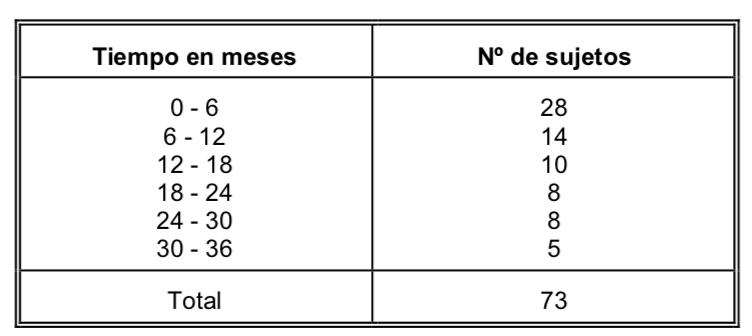
\includegraphics[width=10.44in]{img/1_1}

\textbf{a)} Calcule las frecuencias relativas y porcentajes de los distintos intervalos.

\textbf{b)} Calcule los puntos medios de los intervalos.

\textbf{c)} Calcule las frecuencias absolutas y porcentajes acumulados

\textbf{d)} Construya el histograma, polígono de frecuencias y polígono acumulativo

\hypertarget{soluciuxf3n-4}{%
\subsection{Solución}\label{soluciuxf3n-4}}

\textbf{a), b) y c)}

\begin{itemize}
\tightlist
\item
  f: frecuencias absolutas
\item
  h: frecuencias relativas (porcentajes)
\item
  F: frecuencias absolutas acumuladas
\item
  H: frecuencias relativas acumuladas (en porcentaje)
\end{itemize}

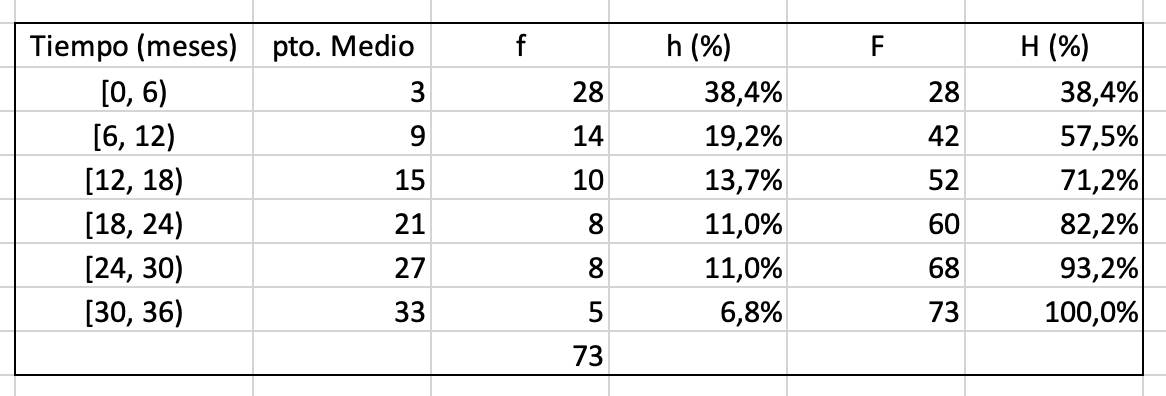
\includegraphics[width=16.19in]{img/1_2}

Tabla construida siguiendo esta \href{https://1fjmanzano.github.io/bioestadistica/tablas-de-frecuencias.html\#tabla-de-frecuencias-pr\%C3\%A1ctica-con-excel}{Práctica con Excel© del Curso de Bioestadística}

\textbf{d)}

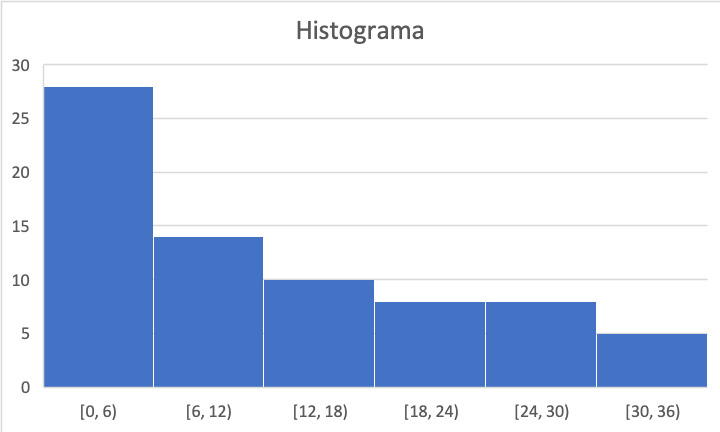
\includegraphics[width=10in]{img/1_3}

Gráfico construido siguiendo esta \href{https://1fjmanzano.github.io/bioestadistica/histogramas.html\#histogramas-con-excel-pr\%C3\%A1cticas}{Práctica con Excel© del Curso de Bioestadística}

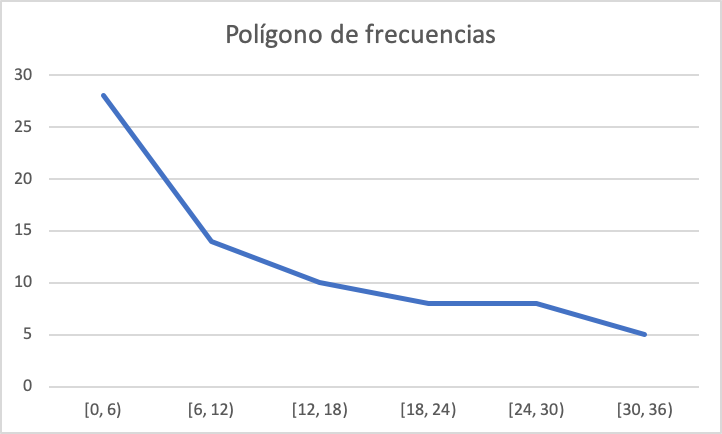
\includegraphics[width=10.03in]{img/1_4}

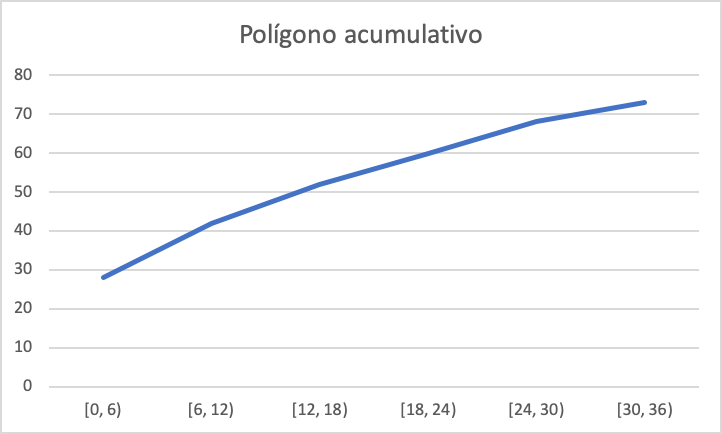
\includegraphics[width=10.03in]{img/1_5}

Gráficos construidos siguiendo esta \href{https://1fjmanzano.github.io/bioestadistica/nu\%CC\%81meros-i\%CC\%81ndices.html\#n\%C3\%BAmeros-\%C3\%ADndices-pr\%C3\%A1ctica-con-excel}{Práctica con Excel© del Curso de Bioestadística}

\hypertarget{pregunta-test-20}{%
\section{Pregunta test}\label{pregunta-test-20}}

Elija la afirmación correcta:

\begin{enumerate}
\def\labelenumi{\alph{enumi})}
\tightlist
\item
  Los valores de cualquier variable deben ser agrupados en intervalos.
\item
  Las variables deben ofrecer valores que no se repitan en los diferentes individuos.
\item
  Las modalidades de una variable deben poder ser observadas en todos los individuos.
\item
  Los individuos pueden poseer diferentes modalidades de la misma variable.
\item
  Todo lo anterior es falso.
\end{enumerate}

Respuesta correcta

\href{https://1fjmanzano.github.io/bioestadistica/tipos-de-variables.html}{Explicación}

\hypertarget{pregunta-test-21}{%
\section{Pregunta test}\label{pregunta-test-21}}

Elija la opción correcta.

\begin{enumerate}
\def\labelenumi{\alph{enumi})}
\tightlist
\item
  Un parámetro es algo calculado sobre cada individuo.
\item
  Un parámetro es calculado sobre la muestra.
\item
  Una variable se calcula sobre los parámetros de una población.
\item
  Un estadístico se calcula sobre la población.
\item
  Nada de lo anterior es correcto.
\end{enumerate}

Respuesta correcta

\href{https://1fjmanzano.github.io/bioestadistica/conceptos-previos.html}{Explicación}

\hypertarget{pregunta-test-22}{%
\section{Pregunta test}\label{pregunta-test-22}}

Disponemos de la distribución de edades de los individuos de una población. El número de ellos que no es mayor de edad, es:

\begin{enumerate}
\def\labelenumi{\alph{enumi})}
\tightlist
\item
  Una frecuencia relativa.
\item
  Una frecuencia absoluta.
\item
  Una frecuencia acumulada.
\item
  Una variable numérica.
\item
  Una variable cualitativa.
\end{enumerate}

Respuesta correcta

\href{https://1fjmanzano.github.io/bioestadistica/tablas-de-frecuencias.html}{Explicación}

\hypertarget{pregunta-test-23}{%
\section{Pregunta test}\label{pregunta-test-23}}

¿Cuál de las siguientes no es una característica de los estudios de cohortes?

\begin{enumerate}
\def\labelenumi{\alph{enumi})}
\tightlist
\item
  Son estudios observacionales
\item
  El criterio de selección de los sujetos es la presencia o no de cnfermedad
\item
  Son estudios longitudinales
\item
  Pueden ser prospectivos o retrospectivos
\end{enumerate}

\begin{enumerate}
\def\labelenumi{\arabic{enumi})}
\setcounter{enumi}{4}
\tightlist
\item
  Tienen direccionalidad hacia delante
\end{enumerate}

Respuesta correcta

\href{https://es.wikipedia.org/wiki/Estudio_de_cohorte}{Explicación}

\hypertarget{pregunta-test-24}{%
\section{Pregunta test}\label{pregunta-test-24}}

Para un estudio epidemiológico sobre dolencias de suelo pélvico en mujeres en la provincia de Albacete, se decide seguir la siguiente estrategia de muestreo: Se elige aleatoriamente 10 poblaciones de la provincia, y en cada una de ellas se elige aleatoriamente 10 calles. Allí se elige aleatoriamente 5 números de la calle y se estudia a las mujeres que aceptan participar. El muestreo es:

\begin{enumerate}
\def\labelenumi{\alph{enumi})}
\tightlist
\item
  Aleatorio simple
\item
  Por conglomerados.
\item
  Estratificado.
\item
  Sistemático.
\item
  Estratificado y por conglomerados.
\end{enumerate}

Respuesta correcta

\href{https://1fjmanzano.github.io/bioestadistica/me\%CC\%81todos-de-muestreo.html}{Explicación}

\hypertarget{problema-5}{%
\section{Problema}\label{problema-5}}

Los datos corresponden a las medidas de tensión arterial sistólica (en mm/Hg) registradas sobre 20 individuos fumadores de más de una cajetilla de cigarrillos diaria:

145, 185, 120, 160, 165, 160, 175, 145, 145, 175, 130, 130, 120, 110, 145, 150, 155, 160, 145, 135

\textbf{a)} Construya la tabla de distribución de frecuencias para los datos originales.

\textbf{b)} Construya la tabla de distribución de frecuencias por intervalos de amplitud 10 mm/Hg.

\textbf{c)} Grafique la distribución de la variable.

\#Solución

\textbf{a)}

Contando \emph{con papel y boli}:

\begin{longtable}[]{@{}cccccccccccc@{}}
\toprule
Tensión & 110 & 120 & 130 & 135 & 145 & 150 & 155 & 160 & 165 & 175 & 185\tabularnewline
\midrule
\endhead
f & 1 & 2 & 2 & 1 & 5 & 1 & 1 & 3 & 1 & 2 & 1\tabularnewline
\bottomrule
\end{longtable}

\textbf{b)}

Se pide ahora considerar intervalos de amplitud 10 mm/Hg. Como el mínimo es 110 y el máximo 185, establecemos 8 intervalos:

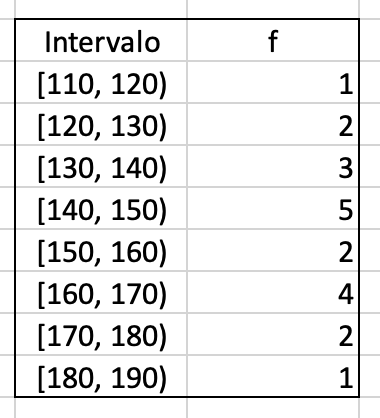
\includegraphics[width=5.28in]{img/1_6}

Tabla construida siguiendo esta \href{https://1fjmanzano.github.io/bioestadistica/tablas-de-frecuencias.html\#tablas-de-frecuencias-pr\%C3\%A1ctica-3-con-excel}{Práctica con Excel© del Curso de Bioestadística}

\textbf{c)} Al tener los datos en intervalos, utilizamos un histograma:

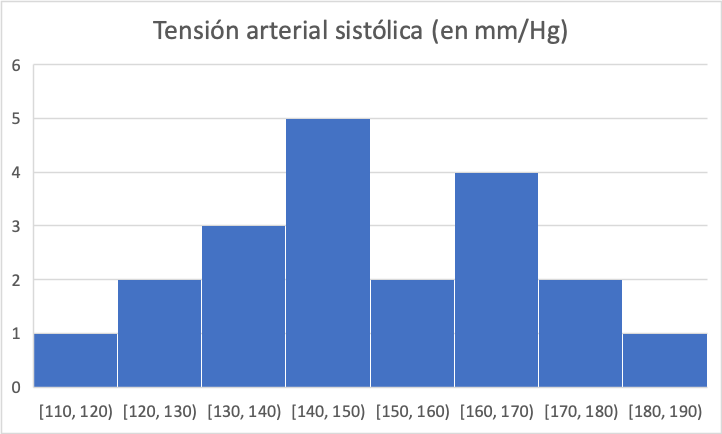
\includegraphics[width=10.03in]{img/1_7}

Gráfico construido siguiendo esta \href{https://1fjmanzano.github.io/bioestadistica/histogramas.html\#histogramas-con-excel-pr\%C3\%A1cticas}{Práctica con Excel© del Curso de Bioestadística}

\hypertarget{pregunta-test-25}{%
\section{Pregunta test}\label{pregunta-test-25}}

Conocemos la distribución de estudiantes entre las distintas facultades del campus Viriato. El número de estudiantes de Enfermería es:

\begin{enumerate}
\def\labelenumi{\alph{enumi})}
\tightlist
\item
  Una frecuencia relativa.
\item
  Una frecuencia absoluta.
\item
  Una frecuencia acumulada.
\item
  Un porcentaje.
\item
  Una variable cualitativa.
\end{enumerate}

Respuesta correcta

\href{https://1fjmanzano.github.io/bioestadistica/tablas-de-frecuencias.html}{Explicación}

\hypertarget{pregunta-test-26}{%
\section{Pregunta test}\label{pregunta-test-26}}

Se llama parámetro a:

\begin{enumerate}
\def\labelenumi{\alph{enumi})}
\tightlist
\item
  Una función de valor numérico definida sobre alguna característica observable en los individuos de una población.
\item
  Una función definida sobre los valores numéricos de una muestra.
\item
  Cualquier variable observable de una población
\item
  Las variables numéricas de la muestra
\item
  Cualquier función sobre las variables observadas
\end{enumerate}

Respuesta correcta

\href{https://1fjmanzano.github.io/bioestadistica/conceptos-previos.html}{Explicación}

\hypertarget{pregunta-test-27}{%
\section{Pregunta test}\label{pregunta-test-27}}

Respecto a los estudios de casos y controles es cierto que:

\begin{enumerate}
\def\labelenumi{\alph{enumi})}
\tightlist
\item
  Se analizan comparando la incidencia de una enfermedad o proceso en el grupo de casos respecto al grupo de controles
\item
  Pueden escogerse varios controles para cada caso
\item
  Una de las medidas de asociación que puede calcularse directamente en su análisis es el riesgo relativo
\item
  Se denominan también estudios de prevalencia
\item
  Es preferible seleccionar casos prevalentes en vez de casos incidentes de la enfermedad o proceso en estudio
\end{enumerate}

Respuesta correcta

\href{https://dsp.facmed.unam.mx/wp-content/uploads/2022/02/Anexo-1C-U-9-Estudios-de-casos-y-controles.-Argimon-J.pdf}{Explicación}

\hypertarget{pregunta-test-28}{%
\section{Pregunta test}\label{pregunta-test-28}}

Si se realiza un estudio para evaluar el rendimiento académico de los estudiantes en una universidad y se selecciona una muestra de estudiantes de manera que cada estudiante tenga la misma probabilidad de ser elegido, ¿qué tipo de muestreo se está utilizando?

\begin{enumerate}
\def\labelenumi{\alph{enumi})}
\tightlist
\item
  Muestreo por conglomerados o por grupos
\item
  Muestreo sistemático
\item
  Muestreo aleatorio simple
\item
  Muestreo no probabilístico
\item
  Muestreo estratificado
\end{enumerate}

Respuesta correcta

\hypertarget{pregunta-test-29}{%
\section{Pregunta test}\label{pregunta-test-29}}

El grado de satisfacción (poco/regular/mucho) con la política española la trataría como:

\begin{enumerate}
\def\labelenumi{\alph{enumi})}
\tightlist
\item
  una variable cualitativa nominal.
\item
  una variable cuantitativa discreta.
\item
  una variable cualitativa ordinal.
\item
  una variable numérica continua.
\item
  ninguna de las anteriores es correcta.
\end{enumerate}

Respuesta correcta

\href{https://1fjmanzano.github.io/bioestadistica/tipos-de-variables.html}{Explicación}

\hypertarget{pregunta-test-30}{%
\section{Pregunta test}\label{pregunta-test-30}}

Con respecto a la modalidades de una variable cualquiera:

\begin{enumerate}
\def\labelenumi{\alph{enumi})}
\tightlist
\item
  Pueden siempre agruparse en clases.
\item
  Deben formar un sistema exhaustivo.
\item
  No pueden agruparse en intervalos.
\item
  No tienen porqué formar un sistema excluyente.
\item
  Solo dos son correctas.
\end{enumerate}

Respuesta correcta

\href{https://1fjmanzano.github.io/bioestadistica/tipos-de-variables.html}{Explicación}

\hypertarget{pregunta-test-31}{%
\section{Pregunta test}\label{pregunta-test-31}}

¿Cuál es el estudio de elección para evaluar la eficacia de un nuevo tratamiento?

\begin{enumerate}
\def\labelenumi{\alph{enumi})}
\tightlist
\item
  Estudio de casos y controles
\item
  Ensayo clínico aleatorio
\item
  Estudio transversal
\item
  Estudio de morbilidad
\item
  Estudio de cohortes
\end{enumerate}

Respuesta correcta

\href{https://www.cancer.gov/espanol/publicaciones/diccionarios/diccionario-cancer/def/ensayo-clinico-aleatorizado}{Explicación}

\hypertarget{pregunta-test-32}{%
\section{Pregunta test}\label{pregunta-test-32}}

Cuando hablamos de número de cumpleaños que ha tenido una persona estamos ante:

\begin{enumerate}
\def\labelenumi{\alph{enumi})}
\tightlist
\item
  Una variable cualitativa ordinal.
\item
  Una variable cualitativa nominal.
\item
  Una variable cuantitativa discreta.
\item
  Una variable cuantitativa continua.
\item
  El número de cumpleaños no es una variable.
\end{enumerate}

Respuesta correcta

\href{https://1fjmanzano.github.io/bioestadistica/tipos-de-variables.html}{Explicación}

\hypertarget{pregunta-test-33}{%
\section{Pregunta test}\label{pregunta-test-33}}

Las pruebas de cribado son una actividad de:

\begin{enumerate}
\def\labelenumi{\alph{enumi})}
\tightlist
\item
  Prevención primaria
\item
  Prevención secundaria
\item
  Prevención terciaria
\item
  Promoción de la salud
\item
  Prevención primaria y promoción de la salud
\end{enumerate}

Respuesta correcta

\href{https://es.wikipedia.org/wiki/Prevención_secundaria}{Explicación}

\hypertarget{pregunta-test-34}{%
\section{Pregunta test}\label{pregunta-test-34}}

Las frecuencias acumuladas tienen sentido para:

\begin{enumerate}
\def\labelenumi{\alph{enumi})}
\tightlist
\item
  Variables ordinales
\item
  Variables numéricas
\item
  Variables nominales
\item
  Todas son correctas.
\item
  Las opciones a) y b) son correctas.
\end{enumerate}

Respuesta correcta

\href{https://1fjmanzano.github.io/bioestadistica/tablas-de-frecuencias.html}{Explicación}

\hypertarget{pregunta-test-35}{%
\section{Pregunta test}\label{pregunta-test-35}}

Señale la respuesta INCORRECTA respecto a los estudios de cohortes:

\begin{enumerate}
\def\labelenumi{\alph{enumi})}
\tightlist
\item
  Pueden ser prospectivos y retrospectivos
\item
  Son estudios observacionales y descriptivos
\item
  Permiten establecer con claridad la secuencia temporal de los eventos de interés
\item
  Permiten medir la incidencia de la enfermedad
\item
  Permite medir los efectos de exposiciones infrecuentes en la población
\end{enumerate}

Respuesta correcta

\href{https://es.wikipedia.org/wiki/Estudio_de_cohorte}{Explicación}

\hypertarget{pregunta-test-36}{%
\section{Pregunta test}\label{pregunta-test-36}}

Disponemos de la distribución de edades de los individuos de una población. El número de ellos que tiene dos o menos hijos es:

\begin{enumerate}
\def\labelenumi{\alph{enumi})}
\tightlist
\item
  Una variable cualitativa.
\item
  Una variable numérica.
\item
  Una frecuencia acumulada.
\item
  Son correctas a) y b)
\item
  Ninguna es correcta.
\end{enumerate}

Respuesta correcta

\href{https://1fjmanzano.github.io/bioestadistica/tablas-de-frecuencias.html}{Explicación}

\hypertarget{pregunta-test-37}{%
\section{Pregunta test}\label{pregunta-test-37}}

Deseamos conocer la opinión de los ciudadanos de Málaga sobre el sistema de salud pública. Para ello elegimos una muestra aleatoria de entre los abonados a telefónica. Entonces:

\begin{enumerate}
\def\labelenumi{\alph{enumi})}
\tightlist
\item
  La población de estudio es la de los ciudadanos de Málaga.
\item
  La población de estudio es la de los abonados a telefónica.
\item
  La población objetivo es la de los abonados a telefónica.
\item
  El conjunto de abonados a telefónica son la muestra.
\item
  Nada de lo anterior es cierto.
\end{enumerate}

Respuesta correcta

\href{https://1fjmanzano.github.io/bioestadistica/conceptos-previos.html}{Explicación}

\hypertarget{pregunta-test-38}{%
\section{Pregunta test}\label{pregunta-test-38}}

Los principales objetivos de la estadística descriptiva son:

\begin{enumerate}
\def\labelenumi{\alph{enumi})}
\tightlist
\item
  Sintetizar la información contenida en los datos.
\item
  Aportar resúmenes significativos de las distribuciones.
\item
  Contribuye a la realización de los posteriores análisis estadísticos.
\item
  Todos son correctos.
\end{enumerate}

Respuesta correcta

\href{https://1fjmanzano.github.io/bioestadistica/an\%C3\%A1lisis-exploratorio-de-datos.html}{Explicación}

\hypertarget{pregunta-test-39}{%
\section{Pregunta test}\label{pregunta-test-39}}

Se diseña un estudio para evaluar el efecto sobre la salud de la exposición a los teléfonos móviles en el que durante 10 años se sigue a una población inicialmente sana ¿Qué tipo de diseño tiene ese estudio?

\begin{enumerate}
\def\labelenumi{\alph{enumi})}
\tightlist
\item
  Estudio casos y controles
\item
  Estudio de cohortes
\item
  Estudio transversal
\item
  Estudio de casos
\item
  Ensayo controlado
\end{enumerate}

Respuesta correcta

\href{https://es.wikipedia.org/wiki/Estudio_de_cohorte}{Explicación}

\hypertarget{problema-6}{%
\section{Problema}\label{problema-6}}

Un estudio llevado a cabo por el Pew Research Center's Internet \& American Life Project (\url{http://www.pewinternet.org}) tiene como objetivo analizar la actitud de los jóvenes en EEUU ante las redes sociales y su configuración de la privacidad. Para ello se ha llevado a cabo una encuesta entre usuarios de Facebook. A continuación se muestran dos gráficas con datos de dicho estudio.

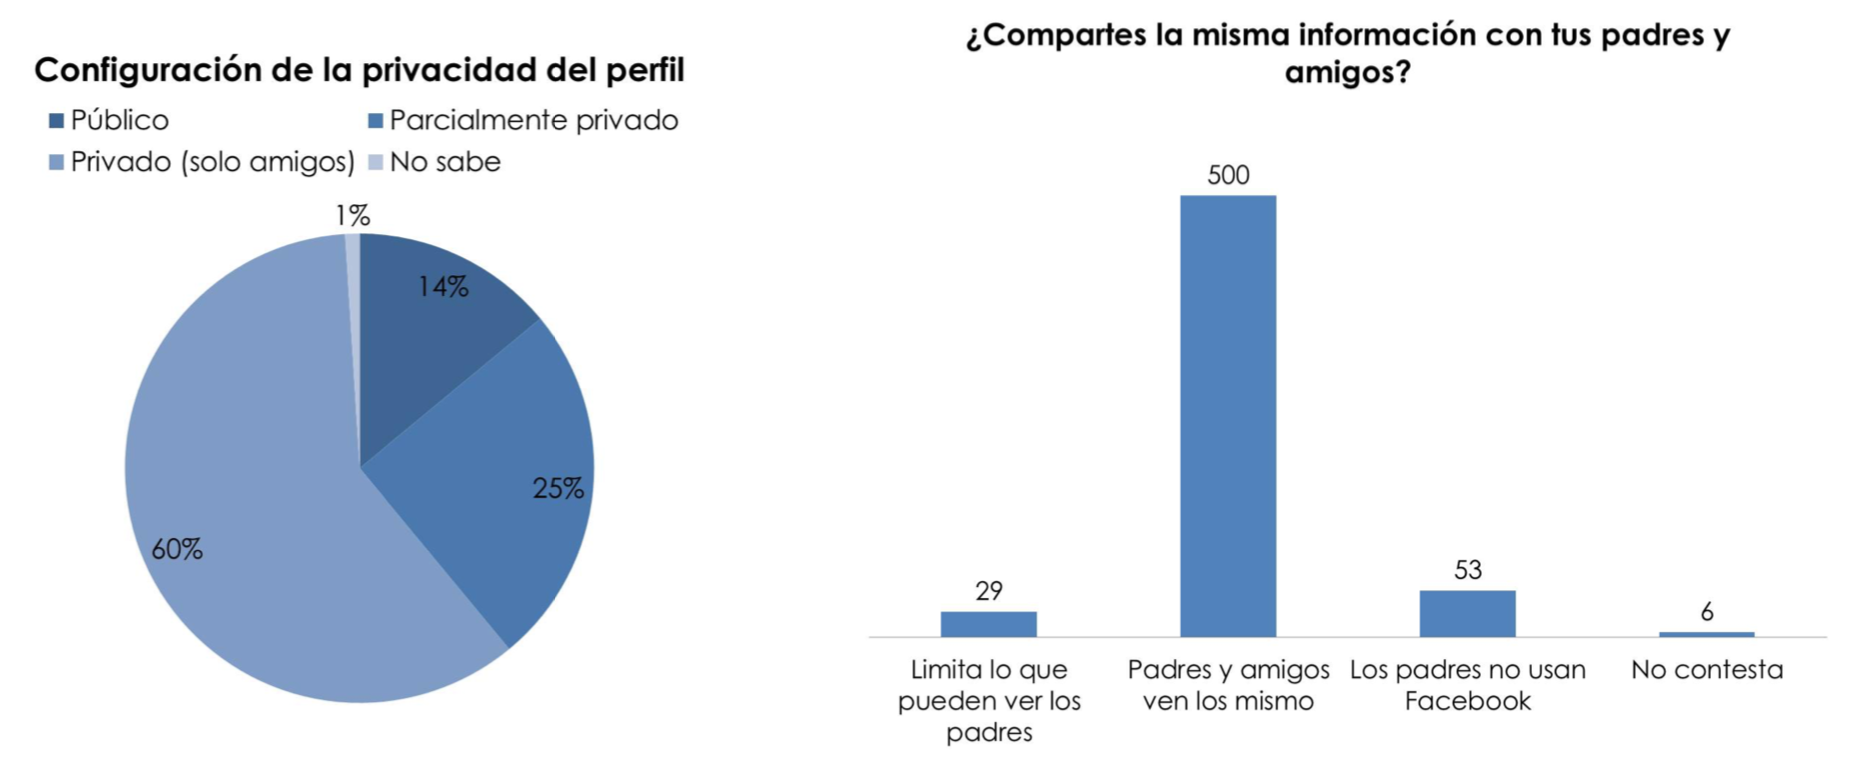
\includegraphics[width=25.81in]{img/1_8}

\textbf{a)} ¿Qué graficas aparecen representadas?¿4A qué tipo de variables hacen referencia?

\textbf{b)} ¿Cuál es el tamaño muestral? ¿Cuántos encuestados tienen su perfil parcialmente privado? ¿Qué porcentaje de usuarios comparte la misma información con sus padres y amigos?

\textbf{c)} Supongamos que les preguntamos a los encuestados cuántos amigos tienen en Facebook. ¿Qué tipo de gráfico crees que deberías utilizar para resumir esa información?

\hypertarget{soluciuxf3n-5}{%
\subsection{Solución}\label{soluciuxf3n-5}}

\textbf{a)} El gráfico de la izquierda es un gráfico de sectores de la variable cualitativa ``Configuración de la privacidad del perfil'' con valores \emph{Público}, \emph{Paccialmente privado}, \emph{Privado (solo amigos} y \emph{No sabe}.

El gráfico de la derecha en una diagrama de barras de la variable cualitativa ``¿Compartes la misma información con tus padres y amigos?'' con valores \emph{Limita lo que pueden ver los padres}, \emph{Padres y amigos ven lo mismo}, \emph{Los padres no usan Facebook} y \emph{No contesta}.

\textbf{b)} El tamaño muestral es la suma de las frecuencias absolutas, es decir, \(29 + 500 + 53 + 6 = 588\).

Hay un 25\% de encuestados que tienen su perfil parcialmente privado, es decir \(0.25 \cdot 588 = 147\).

El porcentaje de usuarios que comparte la misma información con sus padres y amigos es \(\frac{500}{588} \approx 0.8503 = 85\%\).

\textbf{c)} La variable ``Número de amigos en Facebook'' es cuantitativa discreta. Sin embargo, aparecerán muchísimos valores por lo que convendría agrupar los datos en intervalos, entre 0 y 100, entre 100 y 500, entre 500 y 1000 y más de 1000, por ejemplo. De este modo, habría que considerar a la variable como cuantitativa continua y para resumir esa información, usar un histograma.

\hypertarget{pregunta-test-40}{%
\section{Pregunta test}\label{pregunta-test-40}}

En un estudio sobre las causas del cáncer de pulmón se compararon los antecedentes de tabaquismo en los pacientes que habían desarrollado esta enfermedad con los de un grupo de personas y en la enfermedad ¿de qué tipo de estudio epidemiológico se trata?

\begin{enumerate}
\def\labelenumi{\alph{enumi})}
\tightlist
\item
  Estudio de casos y controles
\item
  Estudio de cohortes
\item
  Ensayo clínico aleatorio
\item
  Estudio ecológico
\item
  Estudio transversal
\end{enumerate}

Respuesta correcta

\href{http://www.scielo.org.pe/scielo.php?script=sci_arttext\&pid=S2308-05312020000100138}{Explicación}

\hypertarget{pregunta-test-41}{%
\section{Pregunta test}\label{pregunta-test-41}}

El tipo de variable cualitativa que sus valores o categorías no pueden ser ordenados, se denomina:

\begin{enumerate}
\def\labelenumi{\alph{enumi})}
\tightlist
\item
  Variable ordinal.
\item
  Variable discreta.
\item
  Variable nominal.
\item
  Variable continua.
\end{enumerate}

Respuesta correcta

\href{https://1fjmanzano.github.io/bioestadistica/tipos-de-variables.html}{Explicación}

\hypertarget{pregunta-test-42}{%
\section{Pregunta test}\label{pregunta-test-42}}

Se quiere hacer un estudio sobre el tabaquismo en la Comunidad de Cantabria. Queremos asegurarnos tener cierto número de individuos de la zona litoral, la capital y del interior, pues creemos que en cada una de esas zonas la incidencia es diferente. Haremos un muestreo:

\begin{enumerate}
\def\labelenumi{\alph{enumi})}
\tightlist
\item
  Aleatorio simple.
\item
  Estratificado.
\item
  Sistemático.
\item
  Por grupos.
\item
  No probabilístico.
\end{enumerate}

Respuesta correcta

\hypertarget{pregunta-test-43}{%
\section{Pregunta test}\label{pregunta-test-43}}

¿A qué fase del proceso de investigación pertenece la relación de los objetivos e hipótesis de la investigación?

\begin{enumerate}
\def\labelenumi{\alph{enumi})}
\tightlist
\item
  Fase conceptual.
\item
  Fase Metodológica.
\item
  Fase Empírica.
\item
  Fase de análisis e interpretación de los datos.
\end{enumerate}

Respuesta correcta

\href{https://www.salusplay.com/apuntes/apuntes-metodologia-de-la-investigacion/tema-4-el-proceso-de-investigacion-fases-de-realizacion-de-una-investigacion-cientifica/2}{Explicación}

\hypertarget{pregunta-test-44}{%
\section{Pregunta test}\label{pregunta-test-44}}

Cuál es el estudio de elección para evaluar si existe una relación causa-efecto entre un factor y una enfermedad poco frecuente?

\begin{enumerate}
\def\labelenumi{\alph{enumi})}
\tightlist
\item
  Transversal
\item
  Casos y controles
\item
  Cohortes
\item
  Serie de casos clínicos
\item
  Correlaciones temporales
\end{enumerate}

Respuesta correcta

\href{http://www.scielo.org.pe/scielo.php?script=sci_arttext\&pid=S2308-05312020000100138}{Explicación}

\hypertarget{pregunta-test-45}{%
\section{Pregunta test}\label{pregunta-test-45}}

Para tratar de establecer una relación causal entre el consumo de benzodiacepinas durante el embarazo y el riesgo de fisura palatina en el recién nacido se seleccionan madres de recién nacidos con fisura palatina y se compararon con madres de recién nacidos sanos en cuanto a los antecedentes de toma de benzodiacepinas ¿cuál es el tipo de diseño de estudio empleado?

\begin{enumerate}
\def\labelenumi{\alph{enumi})}
\tightlist
\item
  Casos y controles
\item
  Estudio de cohortes
\item
  Ensayo clínico aleatorizado
\item
  Estudio ecológico
\item
  Ensayo clínico cruzado
\end{enumerate}

Respuesta correcta

\href{http://www.scielo.org.pe/scielo.php?script=sci_arttext\&pid=S2308-05312020000100138}{Explicación}

\hypertarget{pregunta-test-46}{%
\section{Pregunta test}\label{pregunta-test-46}}

Cuando la población objetivo y de estudio en un muestreo difieren mucho, entonces:

\begin{enumerate}
\def\labelenumi{\alph{enumi})}
\tightlist
\item
  Debe usarse el método de respuestas aleatorizadas.
\item
  Pueden existir sesgos.
\item
  No pueden seleccionarse unidades de muestreo.
\item
  Se debe usar un muestreo no probabilístico.
\item
  Nada de lo anterior es correcto.
\end{enumerate}

Respuesta correcta

\href{https://www.cancer.gov/espanol/publicaciones/diccionarios/diccionario-cancer/def/sesgo}{Explicación}

\hypertarget{pregunta-test-47}{%
\section{Pregunta test}\label{pregunta-test-47}}

Un estudio en el que los participantes se asignan al azar para recibir un nuevo tratamiento o placebo se denomina:

\begin{enumerate}
\def\labelenumi{\alph{enumi})}
\tightlist
\item
  Cohortes
\item
  Casos y controles
\item
  Transversal
\item
  Ensayo clínico
\item
  Serie de casos clínicos
\end{enumerate}

Respuesta correcta

\href{https://www.geicam.org/que-hacemos/ensayos-clinicos/que-es-un-ensayo-clinico}{Explicación}

\hypertarget{pregunta-test-48}{%
\section{Pregunta test}\label{pregunta-test-48}}

¿Cómo se denomina el ensayo clínico en el que los pacientes, los investigadores y los profesionales sanitarios implicados sanitarios implicados en la atención de los pacientes desconocen el tratamiento asignado?

\begin{enumerate}
\def\labelenumi{\alph{enumi})}
\tightlist
\item
  Enmascaramiento
\item
  Triple ciego
\item
  Abierto
\item
  Simple ciego
\item
  Doble ciego
\end{enumerate}

Respuesta correcta

\href{http://cv.uoc.edu/UOC/a/moduls/90/90_166d/web/main/m4/22d.html}{Explicación}

\hypertarget{pregunta-test-49}{%
\section{Pregunta test}\label{pregunta-test-49}}

¿A qué se debe el sesgo de selección?

\begin{enumerate}
\def\labelenumi{\alph{enumi})}
\tightlist
\item
  A falta de sinceridad en los individuos de la muestra.
\item
  A las diferencia existente entre diversas muestras.
\item
  A la diferencia entre la población de estudio y la población objetivo.
\item
  A no usar la técnica de respuesta aleatorizada.
\item
  A nada de lo anterior.
\end{enumerate}

Respuesta correcta

\href{https://es.wikipedia.org/wiki/Sesgo_de_selección}{Explicación}

\hypertarget{anuxe1lisis-descriptivo-y-gruxe1fico-de-datos-cuantitativos}{%
\chapter{Análisis Descriptivo y Gráfico de datos cuantitativos}\label{anuxe1lisis-descriptivo-y-gruxe1fico-de-datos-cuantitativos}}

En este capítulo se resolverán problemas relativos a:

\begin{itemize}
\tightlist
\item
  Medidas de tendencia central: Media, Moda, Mediana.
\item
  Medidas de dispersión: Recorrido, Varianza, Desviación típica, Coeficiente de variación, Recorrido intercuartílico. Error estándar.
\item
  Representaciones gráficas: Diagrama de barras, Pictogramas, Cartogramas,
\end{itemize}

\hypertarget{pregunta-test-50}{%
\section{Pregunta test}\label{pregunta-test-50}}

Cuál de las siguientes medidas define mejor la tendencia central de los datos: 5 , 4, 42, 4, 6

\begin{enumerate}
\def\labelenumi{\alph{enumi})}
\tightlist
\item
  La mediana.
\item
  La media.
\item
  El sesgo
\item
  El rango.
\item
  La proporción.
\end{enumerate}

Respuesta correcta

\href{https://1fjmanzano.github.io/bioestadistica/medidas-de-posicio\%CC\%81n-dispersio\%CC\%81n-y-forma.html\#medidas-de-posicio\%CC\%81n-centrales}{Explicación}

\hypertarget{pregunta-test-51}{%
\section{Pregunta test}\label{pregunta-test-51}}

Los diagramas de sectores son muy útiles para comparar:

\begin{enumerate}
\def\labelenumi{\alph{enumi})}
\tightlist
\item
  Dos variables cualitativas en una población.
\item
  Dos variables cuantitativas en una población.
\item
  Una variable cualitativa en dos poblaciones.
\item
  Una variable cuantitativa en dos poblaciones.
\item
  Una variable cuantitativa con otra cualitativa.
\end{enumerate}

Respuesta correcta

\href{https://1fjmanzano.github.io/bioestadistica/diagramas-de-barras-y-sectores.html}{Explicación}

\hypertarget{problema-7}{%
\section{Problema}\label{problema-7}}

El siguiente polígono de frecuencias absolutas acumuladas corresponde a la distribución de frecuencias de la variable \(X\) =``Duración en minutos de una consulta médica especializada''.

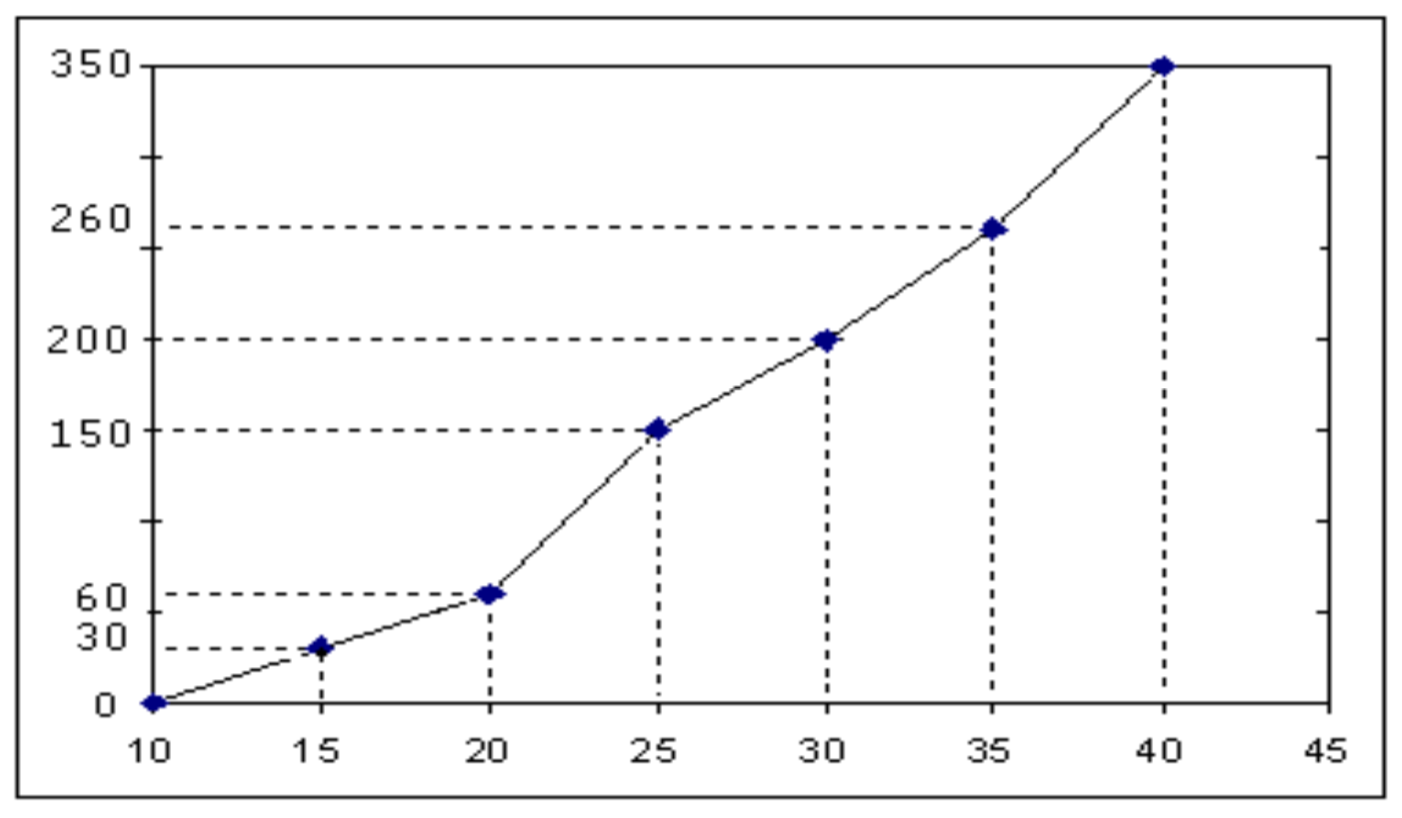
\includegraphics[width=19.47in]{img/2_1}

\textbf{a)} ¿Qué porcentaje de consultas han durado como máximo 30 minutos?

\textbf{b)} ¿Qué porcentaje de consultas han durado entre 25 y 30 minutos?

\hypertarget{soluciuxf3n-6}{%
\subsection{Solución}\label{soluciuxf3n-6}}

Al ser un polígono de frecuencias absolutas acumuladas, vemos que se han contabilizado un total de 350 consultas.

\textbf{a)} Vemos que hay 200 consultas que han durado como máximo 30 minutos. Como \(\frac{200}{350} \approx 0.57\), entonces \textbf{un 57 \% de las consultas han durado entre 25 y 30 minutos}.

\textbf{b)} Entre 25 y 30 minutos, han habido \(200 - 150 = 50\) consultas. Como \(\frac{50}{350} \approx 0.14\), \textbf{un 14 \% de las consultas han durado entre 25 y 30 minutos}

\hypertarget{pregunta-test-52}{%
\section{Pregunta test}\label{pregunta-test-52}}

En cuanto a la presentación ordenada del estudio de una variable aislada:

\begin{enumerate}
\def\labelenumi{\alph{enumi})}
\tightlist
\item
  Lo más informativo es mostrar las medidas de tendencia central.
\item
  Lo más informativo es mostrar las medidas de dispersión.
\item
  Se deben presentar todos los valores observados de la variable, uno a uno, de menor a mayor.
\item
  Las representaciones gráficas dan más información que las tablas de frecuencia.
\item
  A veces no tiene sentido usar frecuencias acumuladas.
\end{enumerate}

Respuesta correcta

\href{https://1fjmanzano.github.io/bioestadistica/otros-gra\%CC\%81ficos.html}{Explicación}

\hypertarget{pregunta-test-53}{%
\section{Pregunta test}\label{pregunta-test-53}}

La mediana es una medida de tendencia central que se usa cuando:

\begin{enumerate}
\def\labelenumi{\alph{enumi})}
\tightlist
\item
  Los datos son impares.
\item
  La muestra es asimétrica.
\item
  La muestra es heterogénea.
\item
  La muestra es simétrica.
\item
  La muestra es homogénea.
\end{enumerate}

Respuesta correcta

\href{https://1fjmanzano.github.io/bioestadistica/medidas-de-posicio\%CC\%81n-dispersio\%CC\%81n-y-forma.html\#medidas-de-posicio\%CC\%81n-centrales}{Explicación}

\hypertarget{pregunta-test-54}{%
\section{Pregunta test}\label{pregunta-test-54}}

El Coeficiente de Variación se calcula:

\begin{enumerate}
\def\labelenumi{\alph{enumi})}
\tightlist
\item
  Multiplicando la Varianza por la Media.
\item
  Dividiendo la Desviación Típica por la Media.
\item
  Dividiendo la Media por la Desviación Típica.
\item
  Dividiendo la Media por la Varianza.
\item
  Multiplicando la Desviación Típica por la Media.
\end{enumerate}

Respuesta correcta

\href{https://es.wikipedia.org/wiki/Coeficiente_de_variación}{Explicación}

\hypertarget{pregunta-test-55}{%
\section{Pregunta test}\label{pregunta-test-55}}

En las representaciones gráficas de variables cualitativas, la regla fundamental a tener en cuenta es:

\begin{enumerate}
\def\labelenumi{\alph{enumi})}
\tightlist
\item
  Las alturas en cada modalidad son proporcionales al valor de la variable.
\item
  Las áreas para cada modalidad son proporcionales al valor de la variable.
\item
  Las áreas para cada modalidad son proporcionales a las frecuencias acumuladas.
\item
  Las áreas para cada modalidad son proporcionales a las frecuencias absolutas o relativas.
\item
  Las alturas para cada modalidad son proporcionales a las frecuencias acumuladas.
\end{enumerate}

Respuesta correcta

\href{https://1fjmanzano.github.io/bioestadistica/diagramas-de-barras-y-sectores.html}{Explicación}

\hypertarget{problema-8}{%
\section{Problema}\label{problema-8}}

En un estudio para evaluar la eficacia de cierto programa educativo sobre salud bucodental, se preguntó a los asistentes con qué frecuencia acudían al dentista por razones preventivas. Dos años después del programa educativo se volvió a preguntar a los asistentes al programa la misma pregunta. En la tabla adjunta se describen los resultados obtenidos:

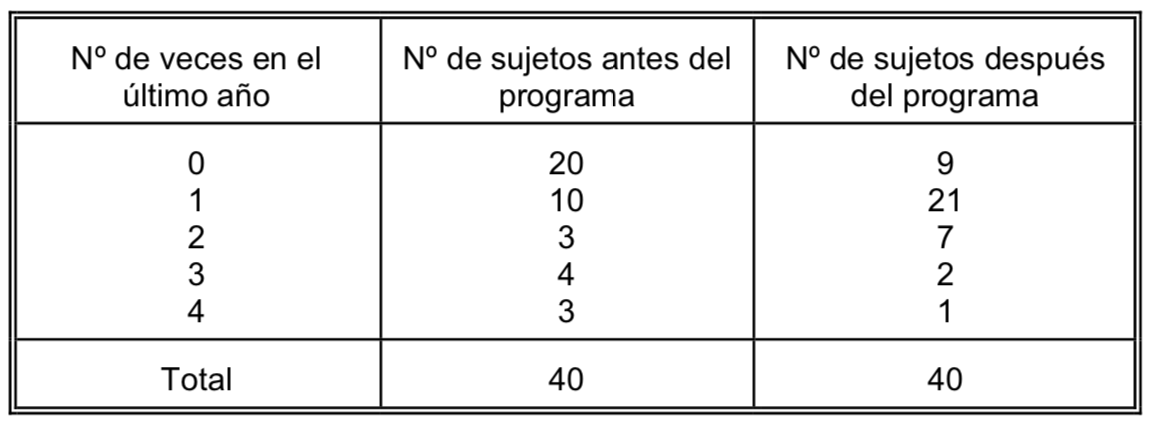
\includegraphics[width=16.06in]{img/2_2}

Construya los diagramas de barras representando gráficamente las distribuciones del número de veces que fueron al dentista en el último año, antes y después del programa educativo. Compare los resultados.

\hypertarget{soluciuxf3n-7}{%
\subsection{Solución}\label{soluciuxf3n-7}}

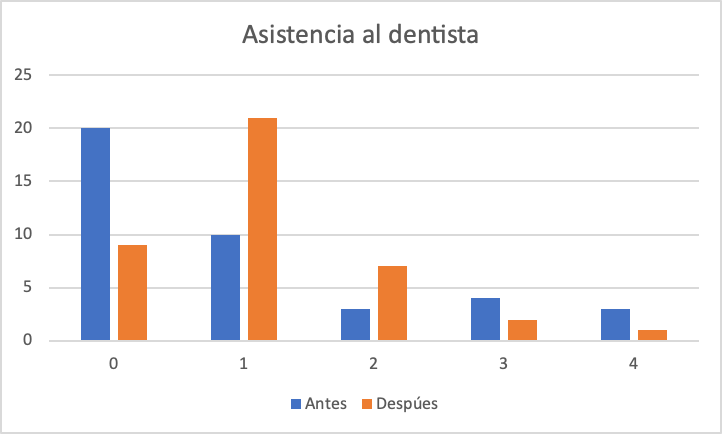
\includegraphics[width=10.03in]{img/2_3}

Gráfico construido siguiendo esta \href{https://1fjmanzano.github.io/bioestadistica/diagramas-de-barras-y-sectores.html}{Práctica con Excel© del Curso de Bioestadística}

Vemos que, antes de participar en el programa, la mayoría de participantes o no acudía al dentista o lo hacía una vez al año. Tras el programa, vemos que ha disminuido drásticamente el número de personas que no acuden al dentista pasando a ser la mayoría los que acuden 1 o 2 veces.

Se observa que, tras el programa, bajan los participantes que acudían 3 o 4 veces.

\hypertarget{pregunta-test-56}{%
\section{Pregunta test}\label{pregunta-test-56}}

Entre las representaciones gráficas para variables cualitativas tenemos:

\begin{enumerate}
\def\labelenumi{\alph{enumi})}
\tightlist
\item
  Histogramas.
\item
  Diagramas integrales.
\item
  Diagramas diferenciales.
\item
  Diagramas de cajas y bigotes.
\item
  Nada de lo anterior.
\end{enumerate}

Respuesta correcta

\begin{enumerate}
\def\labelenumi{\alph{enumi})}
\setcounter{enumi}{3}
\tightlist
\item
  \href{https://1fjmanzano.github.io/bioestadistica/diagramas-de-barras-y-sectores.html}{Explicación}
\end{enumerate}

\hypertarget{pregunta-test-57}{%
\section{Pregunta test}\label{pregunta-test-57}}

A continuación aparecen representados los histogramas y diagramas de cajas de tres conjuntos de datos distintos. Empareja cada histograma con el diagrama de cajas que le corresponde.

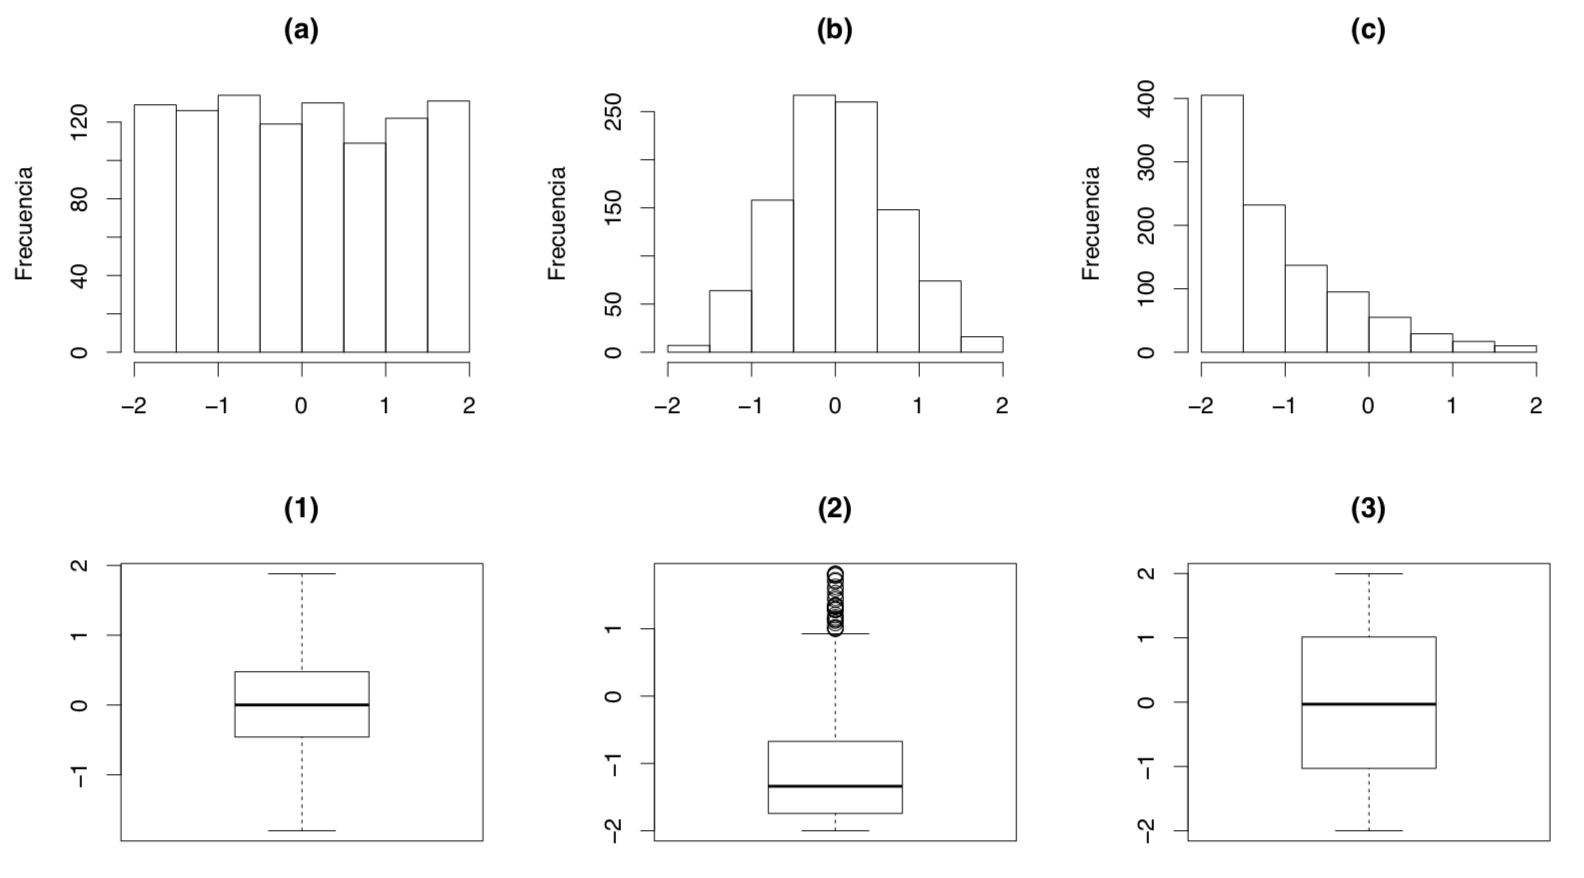
\includegraphics[width=22in]{img/2_8}

\begin{enumerate}
\def\labelenumi{\alph{enumi})}
\tightlist
\item
  a-1, b-2, c-3
\item
  a-3, b-2, c-1
\item
  a-3, b-1, c-2
\item
  a-1, b-3, c-2
\item
  a-2, b-1, c-3
\end{enumerate}

Respuesta correcta

\href{https://1fjmanzano.github.io/bioestadistica/histogramas.html}{Explicación}

\hypertarget{pregunta-test-58}{%
\section{Pregunta test}\label{pregunta-test-58}}

De los siguientes conceptos indique el que no tenga sentido:

\begin{enumerate}
\def\labelenumi{\alph{enumi})}
\tightlist
\item
  Diagrama de barras para la variable ``Grupo sanguíneo''
\item
  Pictograma para la variable ``Altura''
\item
  Diagrama integral para la variable ``Nivel de colesterol''
\item
  Diagrama de sectores para la variable ``Sexo''
\item
  Histograma para la variable ``Peso''
\end{enumerate}

Respuesta correcta

\href{https://1fjmanzano.github.io/bioestadistica/otros-gra\%CC\%81ficos.html}{Explicación}

\hypertarget{problema-9}{%
\section{Problema}\label{problema-9}}

Investigadores de un centro hospitalario planificaron un estudio para determinar la eficacia de cierto complemento dietético en el tratamiento de la artritis reumatoide. El estudio se realizó sobre 50 pacientes con esta enfermedad, administrando a la mitad el complemento dietético y al resto un placebo durante veinte semanas. De los 25 pacientes que recibieron en complemento dietético, 18 presentaron mejoría, mientras que esto ocurrió en 10 de los que recibieron el placebo. Estructure los datos en una tabla de distribución de frecuencias conjuntas y calcule e interprete los porcentajes por filas y columnas.

\hypertarget{soluciuxf3n-8}{%
\subsection{Solución}\label{soluciuxf3n-8}}

Comenzamos escrbiendo la tabla de doble entrada con las variables y los datos proporcionados:

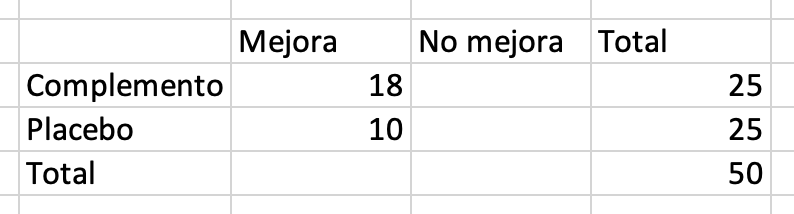
\includegraphics[width=11.03in]{img/2_4}

Completamos los datos y añadimos los prcentajes por filas y columnas.

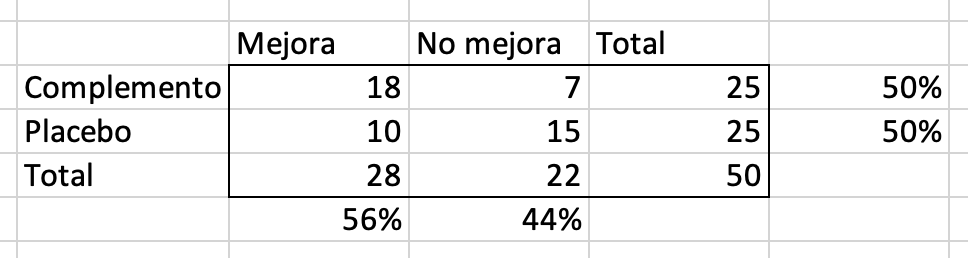
\includegraphics[width=13.44in]{img/2_5}

A la vista de los datos por filas, vemos que se sumistró a la mitad de los participantes el complemento dietético y a la otra mitad el placebo (50 \% vs 50 \%). Por columnas, vemos que un 56 \% de participantes mejoran frente a un 44 \% que no lo hacen. Esta diferencia es debida, sobre todo, al grupo que recibió el complemento donde la mejoría es bastante mayor que en el grupo que recibió el placebo (18 vs 10).

\hypertarget{pregunta-test-59}{%
\section{Pregunta test}\label{pregunta-test-59}}

Si queremos representar gráficamente los porcentajes de una variable cuantitativa continua debemos usar:

\begin{enumerate}
\def\labelenumi{\alph{enumi})}
\tightlist
\item
  Pictogramas
\item
  Diagrama de barras
\item
  Diagrama diferencial acumulado
\item
  Histograma
\item
  No existe gráfica posible
\end{enumerate}

Respuesta correcta

\href{https://1fjmanzano.github.io/bioestadistica/histogramas.html}{Explicación}

\hypertarget{pregunta-test-60}{%
\section{Pregunta test}\label{pregunta-test-60}}

Los gráficos indicados para variables cualitativas son:

\begin{enumerate}
\def\labelenumi{\alph{enumi})}
\tightlist
\item
  Los diagramas de barras y los histogramas
\item
  Los diagramas de barras, los de sectores y los pictogramas
\item
  Los histogramas y pictogramas
\item
  Sólo los diagramas de barras
\item
  Los diagramas integrales
\end{enumerate}

Respuesta correcta

\href{https://1fjmanzano.github.io/bioestadistica/diagramas-de-barras-y-sectores.html}{Explicación}

\hypertarget{problema-10}{%
\section{Problema}\label{problema-10}}

El volumen corpuscular medio (VCM) es uno de los parámetros calculados en un examen de conteo sanguíneo completo. El VCM indica el tamaño de los glóbulos rojos y se mide en fentolitros. A continuación se muestran los valores de VCM de 19 pacientes que se han sometido a un examen de conteo sanguíneo completo.

83; 77; 82; 84; 85; 92; 92; 93; 91; 86; 89; 109; 81; 79; 81; 88; 110; 90; 80:

\textbf{a)} Construye la tabla de frecuencias y representa el histograma correspondiente.

\textbf{b)} Dibuja el boxplot de estos datos.

\textbf{a)} Al pedirnos el histograma, tenemos que agrupar los datos en intervalos. Vemos que el valor mínimo es 77 y el máximo 110. Así, vamos aconsiderar intervalos de amplitud 5 comenzando por el intervalos \([75,80)\). En el último intervalos, incluimos al extremo superior \(110\):

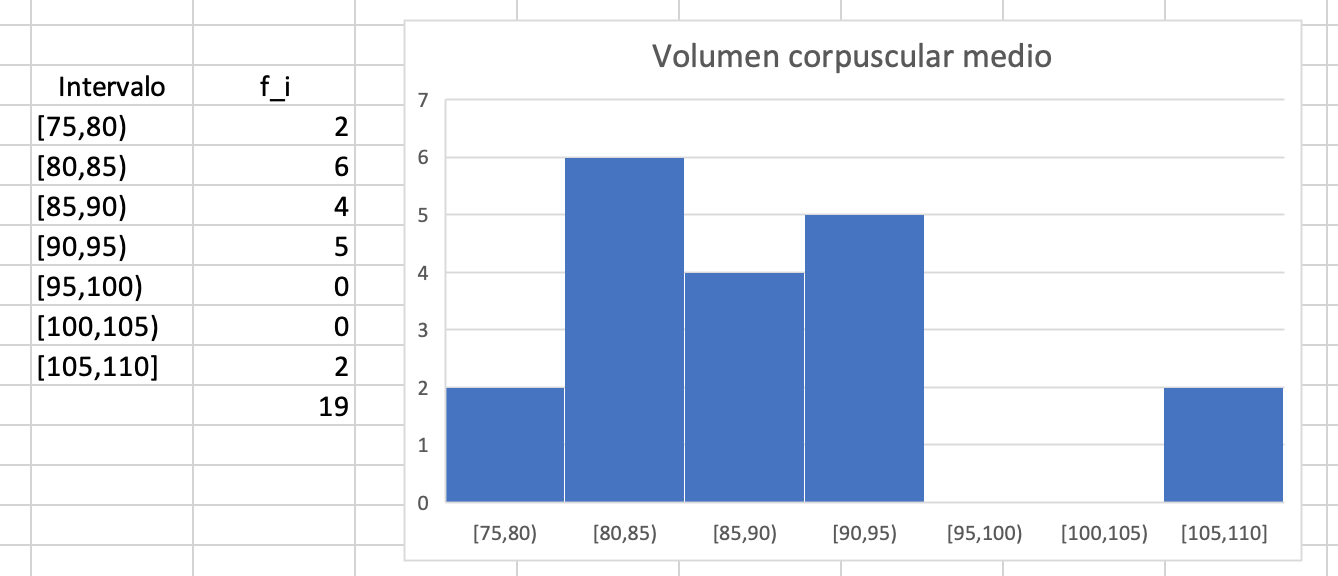
\includegraphics[width=18.58in]{img/2_6}

Gráfico obtenido siguiendo esta \href{https://1fjmanzano.github.io/bioestadistica/histogramas.html\#histogramas-con-excel-pr\%C3\%A1cticas}{Práctica del Curso de Bioestadística}

\textbf{b)} Obtenemos el boxplot (diagrama de cajas y bigotes) con Excel©

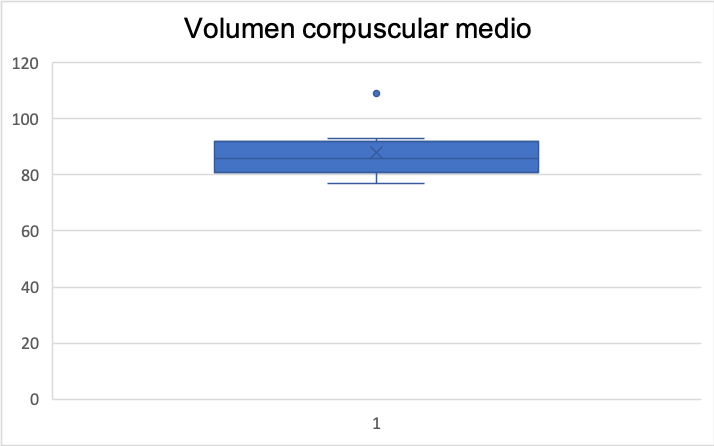
\includegraphics[width=9.92in]{img/2_7}

\hypertarget{pregunta-test-61}{%
\section{Pregunta test}\label{pregunta-test-61}}

¿Qué gráfico elegirías para representar una las respuestas a una encuesta sobre el número de hijos que tiene la población?

\begin{enumerate}
\def\labelenumi{\alph{enumi})}
\tightlist
\item
  Histograma
\item
  Diagrama de sectores
\item
  Pictograma
\item
  Diagrama de Barras
\item
  Ninguna de las anteriores
\end{enumerate}

Respuesta correcta

\href{https://1fjmanzano.github.io/bioestadistica/diagramas-de-barras-y-sectores.html}{Explicación}

\hypertarget{pregunta-test-62}{%
\section{Pregunta test}\label{pregunta-test-62}}

Para comparar la variabilidad relativa de la tensión arterial diastólica y el nivel de colesterol en sangre de una serie de individuos, utilizamos

\begin{enumerate}
\def\labelenumi{\alph{enumi})}
\tightlist
\item
  Las desviaciones típicas.
\item
  Los rangos.
\item
  Los coeficientes de variación.
\item
  La diferencia de las medias.
\item
  La diferencia de las varianzas.
\end{enumerate}

Respuesta correcta

\href{https://1fjmanzano.github.io/bioestadistica/medidas-de-posicio\%CC\%81n-dispersio\%CC\%81n-y-forma.html}{Explicación}

\hypertarget{pregunta-test-63}{%
\section{Pregunta test}\label{pregunta-test-63}}

La media aritmética de una variable cuantitativa:

\begin{enumerate}
\def\labelenumi{\alph{enumi})}
\tightlist
\item
  Es siempre un valor de la variable.
\item
  No tiene sentido calcularla para variables discretas.
\item
  Es el valor más representativo de una modalidad.
\item
  Si la variable es discreta, puede no ser única.
\item
  Existe siempre.
\end{enumerate}

Respuesta correcta

\href{https://1fjmanzano.github.io/bioestadistica/medidas-de-posicio\%CC\%81n-dispersio\%CC\%81n-y-forma.html\#medidas-de-posicio\%CC\%81n-centrales}{Explicación}

\hypertarget{pregunta-test-64}{%
\section{Pregunta test}\label{pregunta-test-64}}

Las siguientes medidas son todas de centralización, excepto:

\begin{enumerate}
\def\labelenumi{\alph{enumi})}
\tightlist
\item
  La media.
\item
  La moda.
\item
  La mediana.
\item
  Rango intercuartílico.
\item
  El percentil 50.
\end{enumerate}

Respuesta correcta

\href{https://1fjmanzano.github.io/bioestadistica/medidas-de-posicio\%CC\%81n-dispersio\%CC\%81n-y-forma.html\#medidas-de-posicio\%CC\%81n-centrales}{Explicación}

\hypertarget{pregunta-test-65}{%
\section{Pregunta test}\label{pregunta-test-65}}

En un estudio descriptivo se obtiene una que el peso tiene una media de 60 kg y una desviación típica de 20 kg., mientras que la media de las edades es 15 años, con una desviación típica de 5 años. Entonces:

\begin{enumerate}
\def\labelenumi{\alph{enumi})}
\tightlist
\item
  Hay más dispersión en pesos que en edades.
\item
  Hay más dispersión en edades que en pesos.
\item
  Peso y edad están dispersos de modo equivalente.
\item
  No tiene sentido compararlos al no coincidir las unidades de medida.
\item
  Para comparar ambas dispersiones debemos usar la covarianza.
\end{enumerate}

Respuesta correcta

\href{https://1fjmanzano.github.io/bioestadistica/medidas-de-posicio\%CC\%81n-dispersio\%CC\%81n-y-forma.html}{Explicación}

\hypertarget{pregunta-test-66}{%
\section{Pregunta test}\label{pregunta-test-66}}

¿Cuál de las siguientes características no se corresponde con el concepto de mediana?

\begin{enumerate}
\def\labelenumi{\alph{enumi})}
\tightlist
\item
  Es el centro de gravedad de la distribución.
\item
  No se ve afectada por los valores extremos.
\item
  Deja por debajo el mismo número de datos que por encima.
\item
  Es el segundo cuartil.
\item
  Todo lo anterior se corresponde con la mediana.
\end{enumerate}

Respuesta correcta

\href{https://1fjmanzano.github.io/bioestadistica/medidas-de-posicio\%CC\%81n-dispersio\%CC\%81n-y-forma.html\#medidas-de-posicio\%CC\%81n-centrales}{Explicación}

\hypertarget{pregunta-test-67}{%
\section{Pregunta test}\label{pregunta-test-67}}

Señale cuál de las siguientes afirmaciones es falsa:

\begin{enumerate}
\def\labelenumi{\alph{enumi})}
\tightlist
\item
  La media aritmética es siempre el centro de gravedad de la distribución.
\item
  En una distribución continua simétrica, media y mediana coinciden.
\item
  La media aritmética cambia cuando cambia algún dato.
\item
  La mediana no siempre cambia cuando lo hace algún dato.
\item
  En las distribuciones continuas simétricas todas las medidas de centralización coinciden.
\end{enumerate}

Respuesta correcta

\href{https://www.statisticshowto.com/what-is-a-bimodal-distribution/}{Explicación}

\hypertarget{pregunta-test-68}{%
\section{Pregunta test}\label{pregunta-test-68}}

El coeficiente de variación:

\begin{enumerate}
\def\labelenumi{\alph{enumi})}
\tightlist
\item
  Permite comparar la dispersión de dos poblaciones.
\item
  Es menor que la media.
\item
  Es menor que la desviación típica.
\item
  No depende de la media ni la desviación típica.
\item
  Depende de la escala que se use al medir la variable.
\end{enumerate}

Respuesta correcta

\href{https://en.wikipedia.org/wiki/Coefficient_of_variation}{Explicación}

\hypertarget{pregunta-test-69}{%
\section{Pregunta test}\label{pregunta-test-69}}

Se pide a unos enfermos que valoren su grado de mejoría tras un tratamiento en una escala de 1 a 5. De la siguiente colección de posibilidades, cuál cree que resume mejor los mismos:

\begin{enumerate}
\def\labelenumi{\alph{enumi})}
\tightlist
\item
  Media, Mediana y Moda.
\item
  Percentil 25, Percentil 50, Percentil 75.
\item
  Media y desviación típica.
\item
  Mediana y desviación típica.
\item
  Rango
\end{enumerate}

Respuesta correcta

\href{https://1fjmanzano.github.io/bioestadistica/medidas-de-posicio\%CC\%81n-dispersio\%CC\%81n-y-forma.html\#medidas-de-dispersio\%CC\%81n}{Explicación}

\hypertarget{pregunta-test-70}{%
\section{Pregunta test}\label{pregunta-test-70}}

De las siguientes medidas, cuáles podria utilizar para argumentar en favor o en contra de la asimetría de la variable edad:

\begin{enumerate}
\def\labelenumi{\alph{enumi})}
\tightlist
\item
  Percentil 25 y percentil 75.
\item
  Media y Percentil 60.
\item
  Media y mediana
\item
  Media y desviación típica.
\item
  Ninguna de las anteriores.
\end{enumerate}

Respuesta correcta

\href{https://1fjmanzano.github.io/bioestadistica/medidas-de-forma.html}{Explicación}

\hypertarget{pregunta-test-71}{%
\section{Pregunta test}\label{pregunta-test-71}}

La pregunta: ¿qué nivel de colesterol sólo es superado por el 5\% de los individuos?, tiene por respuesta:

\begin{enumerate}
\def\labelenumi{\alph{enumi})}
\tightlist
\item
  El percentil 95.
\item
  El percentil 5.
\item
  Los percentiles 2,5 y 97,5
\item
  95\%.
\item
  Nada de lo anterior.
\end{enumerate}

Respuesta correcta

\href{https://1fjmanzano.github.io/bioestadistica/medidas-de-posicio\%CC\%81n-dispersio\%CC\%81n-y-forma.html\#medidas-de-posicio\%CC\%81n-no-centrales}{Explicación}

\hypertarget{pregunta-test-72}{%
\section{Pregunta test}\label{pregunta-test-72}}

Qué peso no llega a alcanzar el 40\% de los individuos de una población:

\begin{enumerate}
\def\labelenumi{\alph{enumi})}
\tightlist
\item
  El 40\%.
\item
  El 60\%.
\item
  El percentil 60.
\item
  El percentil 40.
\item
  Los percentiles 20 y 60.
\end{enumerate}

Respuesta correcta

\href{https://1fjmanzano.github.io/bioestadistica/medidas-de-posicio\%CC\%81n-dispersio\%CC\%81n-y-forma.html\#medidas-de-posicio\%CC\%81n-no-centrales}{Explicación}

\hypertarget{pregunta-test-73}{%
\section{Pregunta test}\label{pregunta-test-73}}

La media aritmética de una variable discreta:

\begin{enumerate}
\def\labelenumi{\alph{enumi})}
\tightlist
\item
  Puede ser un valor de la variable.
\item
  No debería ser utilizada como medida de centralización.
\item
  Es lo mismo que el percentil 50.
\item
  Puede no ser única.
\item
  Todo lo anterior es falso.
\end{enumerate}

Respuesta correcta

\href{https://1fjmanzano.github.io/bioestadistica/medidas-de-posicio\%CC\%81n-dispersio\%CC\%81n-y-forma.html\#medidas-de-posicio\%CC\%81n-centrales}{Explicación}

\hypertarget{pregunta-test-74}{%
\section{Pregunta test}\label{pregunta-test-74}}

Se pregunta a los individuos su opinión sobre una cuestión, pudiendo valorar estos su respuesta en términos de: en contra, en parte a favor, muy a favor, totalmente de acuerdo. Elija la afirmación correcta:

\begin{enumerate}
\def\labelenumi{\alph{enumi})}
\tightlist
\item
  Podemos calcular la media.
\item
  Podemos calcular el coeficiente de variación.
\item
  La variable es de tipo ordinal
\item
  La variable es de tipo cualitativo nominal.
\item
  Nada de lo anterior es cierto.
\end{enumerate}

Respuesta correcta

\href{https://1fjmanzano.github.io/bioestadistica/tipos-de-variables.html}{Explicación}

\hypertarget{pregunta-test-75}{%
\section{Pregunta test}\label{pregunta-test-75}}

En una población, el 70\% de las alturas consideradas ``más normales'' se encuentran:

\begin{enumerate}
\def\labelenumi{\alph{enumi})}
\tightlist
\item
  Por encima del percentil 70.
\item
  Por debajo del cuantil 0,30
\item
  Entre el percentil 30 y el 70
\item
  Entre el percentil 15 y el 85.
\item
  Entre la media y la mediana.
\end{enumerate}

Respuesta correcta

\href{https://1fjmanzano.github.io/bioestadistica/distribuciones-de-probabilidad.html\#distribucio\%CC\%81n-normal}{Explicación}

\hypertarget{pregunta-test-76}{%
\section{Pregunta test}\label{pregunta-test-76}}

Las medidas de centralización, en cuanto a la información que ofrecen sobre una variable numérica, preferimos (por orden, de peor a mejor):

\begin{enumerate}
\def\labelenumi{\alph{enumi})}
\tightlist
\item
  media, mediana, moda
\item
  moda, media, mediana
\item
  media, moda, mediana.
\item
  No se puede en general recomendar una como mejor que las otras.
\item
  Todo lo anterior es falso.
\end{enumerate}

Respuesta correcta

\href{https://1fjmanzano.github.io/bioestadistica/medidas-de-posicio\%CC\%81n-dispersio\%CC\%81n-y-forma.html\#medidas-de-posicio\%CC\%81n-centrales}{Explicación}

\hypertarget{pregunta-test-77}{%
\section{Pregunta test}\label{pregunta-test-77}}

Si una muestra posee valores anómalos, de las siguientes cuál usarías como medida de dispersión:

\begin{enumerate}
\def\labelenumi{\alph{enumi})}
\tightlist
\item
  Varianza.
\item
  Desviación típica.
\item
  Rango intercuartílico.
\item
  Rango.
\item
  Máximo y coeficiente de variación.
\end{enumerate}

Respuesta correcta

\href{https://1fjmanzano.github.io/bioestadistica/medidas-de-posicio\%CC\%81n-dispersio\%CC\%81n-y-forma.html\#medidas-de-dispersio\%CC\%81n}{Explicación}

\hypertarget{pregunta-test-78}{%
\section{Pregunta test}\label{pregunta-test-78}}

Si queremos saber cómo de disperso está una variable relativamente con respecto a la magnitud de los valores centrales de la misma, usaremos:

\begin{enumerate}
\def\labelenumi{\alph{enumi})}
\tightlist
\item
  Varianza.
\item
  Desviación típica.
\item
  Rango intercuartílico.
\item
  Rango.
\item
  Coeficiente de variación.
\end{enumerate}

Respuesta correcta

\href{https://en.wikipedia.org/wiki/Coefficient_of_variation}{Explicación}

\hypertarget{pregunta-test-79}{%
\section{Pregunta test}\label{pregunta-test-79}}

Si el coeficiente de asimetría en una población presenta el valor 0,99 entonces:

\begin{enumerate}
\def\labelenumi{\alph{enumi})}
\tightlist
\item
  La distribución presenta una cola a la derecha.
\item
  La distribución presenta una cola a la izquierda.
\item
  La distribución es más apuntada que la normal.
\item
  La distribución es menos apuntada que la normal.
\item
  La distribución es prácticamente simétrica.
\end{enumerate}

Respuesta correcta

\href{https://1fjmanzano.github.io/bioestadistica/medidas-de-forma.html}{Explicación}

\hypertarget{pregunta-test-80}{%
\section{Pregunta test}\label{pregunta-test-80}}

Si la media del peso en una población es 60 kg. y la mediana 65kg., entonces afirmamos que la distribución del peso en la población es:

\begin{enumerate}
\def\labelenumi{\alph{enumi})}
\tightlist
\item
  Platicúrtica.
\item
  Mesocúrtica.
\item
  Leptocúrtica.
\item
  Asimétrica.
\item
  Unimodal.
\end{enumerate}

Respuesta correcta

\href{https://1fjmanzano.github.io/bioestadistica/medidas-de-forma.html}{Explicación}

\hypertarget{pregunta-test-81}{%
\section{Pregunta test}\label{pregunta-test-81}}

Si el coeficiente de asimetría en una población presenta el valor -5,22 entonces:

\begin{enumerate}
\def\labelenumi{\alph{enumi})}
\tightlist
\item
  La distribución presenta una cola a la derecha.
\item
  La distribución presenta una cola a la izquierda.
\item
  La distribución es más apuntada que la normal.
\item
  La distribución es menos apuntada que la normal.
\item
  Ese valor de asimetría es imposible.
\end{enumerate}

Respuesta correcta

\href{https://1fjmanzano.github.io/bioestadistica/medidas-de-forma.html}{Explicación}

\hypertarget{pregunta-test-82}{%
\section{Pregunta test}\label{pregunta-test-82}}

Medimos el número de glóbulos rojos y el de blancos en cada individuo de una población. Se observa determinada variabilidad en esas cantidades. Queremos saber de qué tipo de célula se presenta mayor variabilidad

\begin{enumerate}
\def\labelenumi{\alph{enumi})}
\tightlist
\item
  Compararemos las desviaciones típicas.
\item
  Compararemos los rangos.
\item
  Estudiaremos la covarianza.
\item
  Estudiaremos el coeficiente de correlación lineal de Pearson.
\item
  Compararemos los coeficientes de variación.
\end{enumerate}

Respuesta correcta

\begin{enumerate}
\def\labelenumi{\alph{enumi})}
\setcounter{enumi}{4}
\tightlist
\item
  \href{https://en.wikipedia.org/wiki/Coefficient_of_variation}{Explicación}
\end{enumerate}

\hypertarget{pregunta-test-83}{%
\section{Pregunta test}\label{pregunta-test-83}}

En una muestra de 1000 mujeres se estudia su número de hijos. Si quiero tener el máximo de información sobre la variable del estudio, preferimos:

\begin{enumerate}
\def\labelenumi{\alph{enumi})}
\tightlist
\item
  Media, Mediana y Moda.
\item
  Percentil 25, Percentil 50, Percentil 75.
\item
  Media y desviación típica.
\item
  Media, mediana, cuartiles, asimetría, curtosis y desviación típica.
\item
  Distribución de frecuencias
\end{enumerate}

Respuesta correcta

\href{https://1fjmanzano.github.io/bioestadistica/tablas-de-frecuencias.html}{Explicación}

\hypertarget{pregunta-test-84}{%
\section{Pregunta test}\label{pregunta-test-84}}

El 3\% de los individuos tiene una altura superior a 190cm. El 5\% mide menos de 150cm. Conocemos:

\begin{enumerate}
\def\labelenumi{\alph{enumi})}
\tightlist
\item
  El percentil 3
\item
  El cuantil 0,06
\item
  El percentil 95
\item
  El percentil 97
\item
  Nada de lo anterior.
\end{enumerate}

Respuesta correcta

\href{https://1fjmanzano.github.io/bioestadistica/medidas-de-posicio\%CC\%81n-dispersio\%CC\%81n-y-forma.html\#medidas-de-posicio\%CC\%81n-no-centrales}{Explicación}

\hypertarget{pregunta-test-85}{%
\section{Pregunta test}\label{pregunta-test-85}}

Respecto a las medidas de centralización:

\begin{enumerate}
\def\labelenumi{\alph{enumi})}
\tightlist
\item
  La media no debe usarse en distribuciones muy asimétricas.
\item
  La moda puede no ser única.
\item
  En distribuciones simétricas media, mediana y moda coinciden.
\item
  Las tres anteriores son correctas.
\item
  Sólo la a) y la b) son correctas
\end{enumerate}

Respuesta correcta

\href{https://1fjmanzano.github.io/bioestadistica/medidas-de-forma.html}{Explicación1} y \href{https://www.statisticshowto.com/what-is-a-bimodal-distribution/}{Explicación2}

\hypertarget{pregunta-test-86}{%
\section{Pregunta test}\label{pregunta-test-86}}

El coeficiente de asimetría en una población vale 3. Elija la afirmación correcta:

\begin{enumerate}
\def\labelenumi{\alph{enumi})}
\tightlist
\item
  La distribución presenta una cola a la derecha.
\item
  La distribución presenta una cola a la izquierda.
\item
  La distribución es simétrica.
\item
  La distribución es más apuntada que la normal
\item
  La media es igual a la mediana.
\end{enumerate}

Respuesta correcta

\href{https://1fjmanzano.github.io/bioestadistica/medidas-de-forma.html}{Explicación}

\hypertarget{pregunta-test-87}{%
\section{Pregunta test}\label{pregunta-test-87}}

¿Cuál de las siguientes medidas define mejor la tendencia central de los datos: 1, 2, 4, 5, 9, 1, 3, 9, 400?

\begin{enumerate}
\def\labelenumi{\alph{enumi})}
\tightlist
\item
  Media.
\item
  Cuantil 0,5.
\item
  Moda
\item
  Desviación típica.
\item
  Ninguna de las anteriores.
\end{enumerate}

Respuesta correcta

\href{https://1fjmanzano.github.io/bioestadistica/medidas-de-posicio\%CC\%81n-dispersio\%CC\%81n-y-forma.html\#medidas-de-posicio\%CC\%81n-no-centrales}{Explicación}

\hypertarget{pregunta-test-88}{%
\section{Pregunta test}\label{pregunta-test-88}}

De las siguientes variables ¿con cuáles NO puedo calcular la media?

\begin{enumerate}
\def\labelenumi{\alph{enumi})}
\tightlist
\item
  temperatura corporal
\item
  pH del estómago
\item
  grupo sanguíneo
\item
  número de glóbulos rojos
\item
  edad
\end{enumerate}

Respuesta correcta

\begin{enumerate}
\def\labelenumi{\alph{enumi})}
\setcounter{enumi}{2}
\tightlist
\item
  \href{https://1fjmanzano.github.io/bioestadistica/tipos-de-variables.html}{Explicación}
\end{enumerate}

\hypertarget{pregunta-test-89}{%
\section{Pregunta test}\label{pregunta-test-89}}

De las siguientes variables con cuál sería menos adecuado un diagrama de barras?

\begin{enumerate}
\def\labelenumi{\alph{enumi})}
\tightlist
\item
  Número de hijos
\item
  Número de coches que posee la familia
\item
  Número de cigarros fumados al día
\item
  Número de glóbulos rojos
\item
  Número de mascotas.
\end{enumerate}

Respuesta correcta

\href{https://1fjmanzano.github.io/bioestadistica/representaciones-gra\%CC\%81ficas.html}{Explicación}

\hypertarget{pregunta-test-90}{%
\section{Pregunta test}\label{pregunta-test-90}}

Cuál es la mediana de los siguientes datos 22, 5, 9, 11, 10, 14, 7

\begin{enumerate}
\def\labelenumi{\alph{enumi})}
\tightlist
\item
  5
\item
  9
\item
  11
\item
  10
\item
  14
\end{enumerate}

Respuesta correcta

\href{https://1fjmanzano.github.io/bioestadistica/medidas-de-posicio\%CC\%81n-dispersio\%CC\%81n-y-forma.html\#medidas-de-posicio\%CC\%81n-centrales}{Explicación}

\hypertarget{pregunta-test-91}{%
\section{Pregunta test}\label{pregunta-test-91}}

Si el cuantil 0,9 del peso es 70 kilogramos, quiere decir esto:

\begin{enumerate}
\def\labelenumi{\alph{enumi})}
\tightlist
\item
  Que una frecuencia del 70\% individuos pesa más de 70 kilogramos.
\item
  Que una frecuencia del 90\% de individuos pesa más de 70 kilogramos.
\item
  Que una frecuencia del 90\% individuos pesa menos de 70 kilogramos.
\item
  Que una frecuencia de 70\% de individuos pesa menos de 90 kilogramos.
\item
  Todas son falsas.
\end{enumerate}

Respuesta correcta

\href{https://1fjmanzano.github.io/bioestadistica/medidas-de-posicio\%CC\%81n-dispersio\%CC\%81n-y-forma.html\#medidas-de-posicio\%CC\%81n-centrales}{Explicación}

\hypertarget{pregunta-test-92}{%
\section{Pregunta test}\label{pregunta-test-92}}

En una distribución: \(P_{25} = 40\), \(P_{50} =60\) y \(P_{75} =70\).

\begin{enumerate}
\def\labelenumi{\alph{enumi})}
\tightlist
\item
  La distribución es simétrica
\item
  La distribución sugiere asimetría negativa
\item
  La distribución sugiere asimetría positiva
\item
  La distribución es leptocúrtica
\item
  Las opciones a) y d) son ciertas
\end{enumerate}

Respuesta correcta

\href{https://1fjmanzano.github.io/bioestadistica/medidas-de-forma.html}{Explicación}

\hypertarget{pregunta-test-93}{%
\section{Pregunta test}\label{pregunta-test-93}}

En una distribución la mediana es 20 y la media es 26:

\begin{enumerate}
\def\labelenumi{\alph{enumi})}
\tightlist
\item
  Con seguridad hay asimetría negativa
\item
  Con seguridad hay asimetría positiva
\item
  Hay colas hacia la derecha y hacia la izquierda.
\item
  Los datos son simétricos.
\item
  Los datos sugieren una cola hacia la derecha. Habría que estudiarlo con más detalle
\end{enumerate}

Respuesta correcta

\href{https://1fjmanzano.github.io/bioestadistica/medidas-de-forma.html}{Explicación}

\hypertarget{pregunta-test-94}{%
\section{Pregunta test}\label{pregunta-test-94}}

El Rango Intercuartílico:

\begin{enumerate}
\def\labelenumi{\alph{enumi})}
\tightlist
\item
  Es sensible a los datos extremos.
\item
  Es la distancia ente el primer y segundo cuartil.
\item
  Es la raíz cuadrada de la varianza
\item
  Sus unidades son el cuadrado de las variables.
\item
  Mide el grado de dispersión de los datos, independientemente de su causa.
\end{enumerate}

Respuesta correcta

\begin{enumerate}
\def\labelenumi{\alph{enumi})}
\setcounter{enumi}{4}
\tightlist
\item
  \href{https://1fjmanzano.github.io/bioestadistica/medidas-de-posicio\%CC\%81n-dispersio\%CC\%81n-y-forma.html\#medidas-de-dispersio\%CC\%81n}{Explicación}
\end{enumerate}

\hypertarget{anuxe1lisis-inferencial.-aplicaciones.}{%
\chapter{Análisis Inferencial. Aplicaciones.}\label{anuxe1lisis-inferencial.-aplicaciones.}}

En este capítulo se resolverán problemas relativos a:

\begin{itemize}
\tightlist
\item
  Objetivos del estudio, hipótesis de trabajo e hipótesis estadísticas
\item
  Importancia de las distribuciones de probabilidad en el trabajo práctico
\item
  Estimación puntual y por intervalo
\item
  Verificación de las hipótesis de trabajo: contraste de hipótesis
\end{itemize}

\hypertarget{pregunta-test-95}{%
\section{Pregunta test}\label{pregunta-test-95}}

En relación a las técnicas de inferencia estadística, elija la afirmación correcta:

\begin{enumerate}
\def\labelenumi{\alph{enumi})}
\tightlist
\item
  La media poblacional es una estimación puntual.
\item
  La media muestral es un parámetro.
\item
  Sólo se rechaza una hipótesis nula si esta es falsa.
\item
  Un intervalo de confianza es una estimación confidencial de un parámetro.
\item
  Todo lo anterior es falso
\end{enumerate}

Respuesta correcta

\href{https://1fjmanzano.github.io/bioestadistica/estimacio\%CC\%81n-de-para\%CC\%81metros.-intervalos-de-confianza.html}{Explicación}

\hypertarget{pregunta-test-96}{%
\section{Pregunta test}\label{pregunta-test-96}}

Un estudio sobre la efectividad de un fármaco llega a la conclusión de que éste es mejor que el placebo con p\textless0,05 ¿Cuál es la interpretación correcta de este resultado?

\begin{enumerate}
\def\labelenumi{\alph{enumi})}
\tightlist
\item
  Con toda seguridad, el tratamiento es mejor que el placebo.
\item
  La probabilidad de que el nuevo tratamiento sea mejor que el placebo es superior al 95\%.
\item
  El tratamiento es un 95\% más efectivo que el placebo.
\item
  La probabilidad de que el placebo sea mejor que el nuevo fármaco es menor de 5\%.
\item
  Si el tratamiento no fuese efectivo, existe menos del 5\% de probabilidad de observar unas muestras tan contrarias a dicha hipótesis como las obtenidas.
\end{enumerate}

Respuesta correcta

\href{https://1fjmanzano.github.io/bioestadistica/valor-p.html}{Explicación}

\hypertarget{pregunta-test-97}{%
\section{Pregunta test}\label{pregunta-test-97}}

En la Distribución Normal:

\begin{enumerate}
\def\labelenumi{\alph{enumi})}
\tightlist
\item
  El intervalo \(\mu \pm \sigma\) abarca el 68\% del área total.
\item
  El intervalo \(\mu \pm 1.96 \sigma\) abarca el 95\% del área.
\item
  El intervalo \(\mu \pm 2.6\sigma\) abarca el 99\% del área.
\item
  El intervalo \(\mu \pm 2.6\sigma\) NO abarca el 5\% del área.
\item
  Todas son ciertas.
\end{enumerate}

Respuesta correcta

\href{https://1fjmanzano.github.io/bioestadistica/distribuciones-de-probabilidad.html\#distribucio\%CC\%81n-normal}{Explicación1}

\href{https://youtu.be/wWeogWp_bO8}{Explicación2}

\hypertarget{problema-11}{%
\section{Problema}\label{problema-11}}

Sea Z una variable aleatoria normal estándar. Calcula:

\textbf{a)} El área encerrada por la función de densidad entre \(z=0\) y \(z=1.35\)

\textbf{b)} \(P(Z \leq 2)\)

\textbf{c)} \(P(-0:5 \leq Z \leq 2.65)\)

\textbf{d)} El valor de z (z \textgreater{} 0) de manera que el área encerrada entre 0 y z sea 0.2.

\textbf{e)} El valor de z tal que la probabilidad de obtener un valor mayor que z sea 0.1.

\hypertarget{soluciuxf3n-9}{%
\subsection{Solución}\label{soluciuxf3n-9}}

Para resolver estas cuestiones, se puede hacer uso de \href{https://youtu.be/xCBUdpIUx18}{la tabla de la Normal Tipificada}, o programas como \href{https://youtu.be/bTnVHL9yG8o?si=I3fjGEwCmzLlbQrI}{Excel© y la app Probability Distributions}.

En este caso, vamos a utilizar el recurso \href{https://www.geogebra.org/calculator}{Geogebra: Calculadora de Probabilidad}. No tenemos más que introducir los datos y obtendremos las soluciones pedidas. Como el problema hace referencia a la distribución \(Z \equiv N(0,1)\), usamos la distribución Normal, como parámetro \(\mu\) pondremos 0 y como parámetro \$\sigma \$ pondremos 1.

\textbf{a)} Solución: \(P(0 \leq Z \leq 1.35) = 0.4115\)

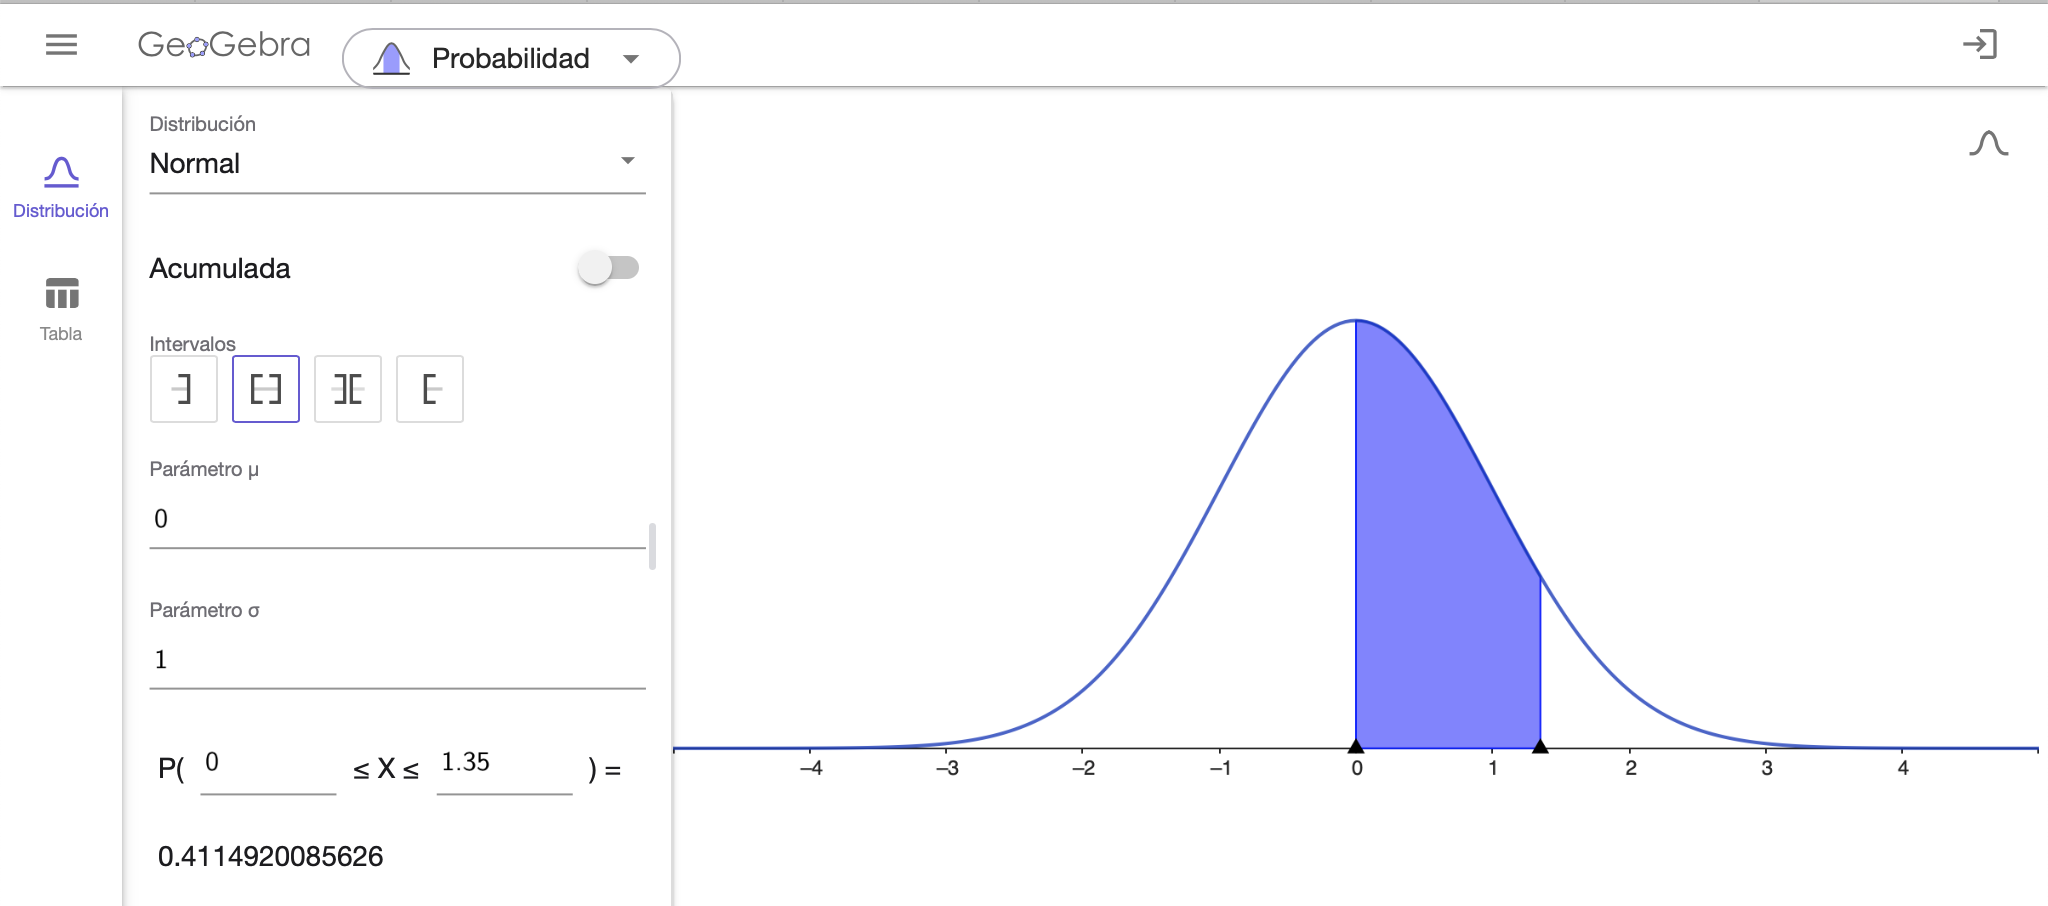
\includegraphics[width=28.44in]{img/3_4}

\textbf{b)} Solución: \(P(Z \leq 2) = 0.9772\)

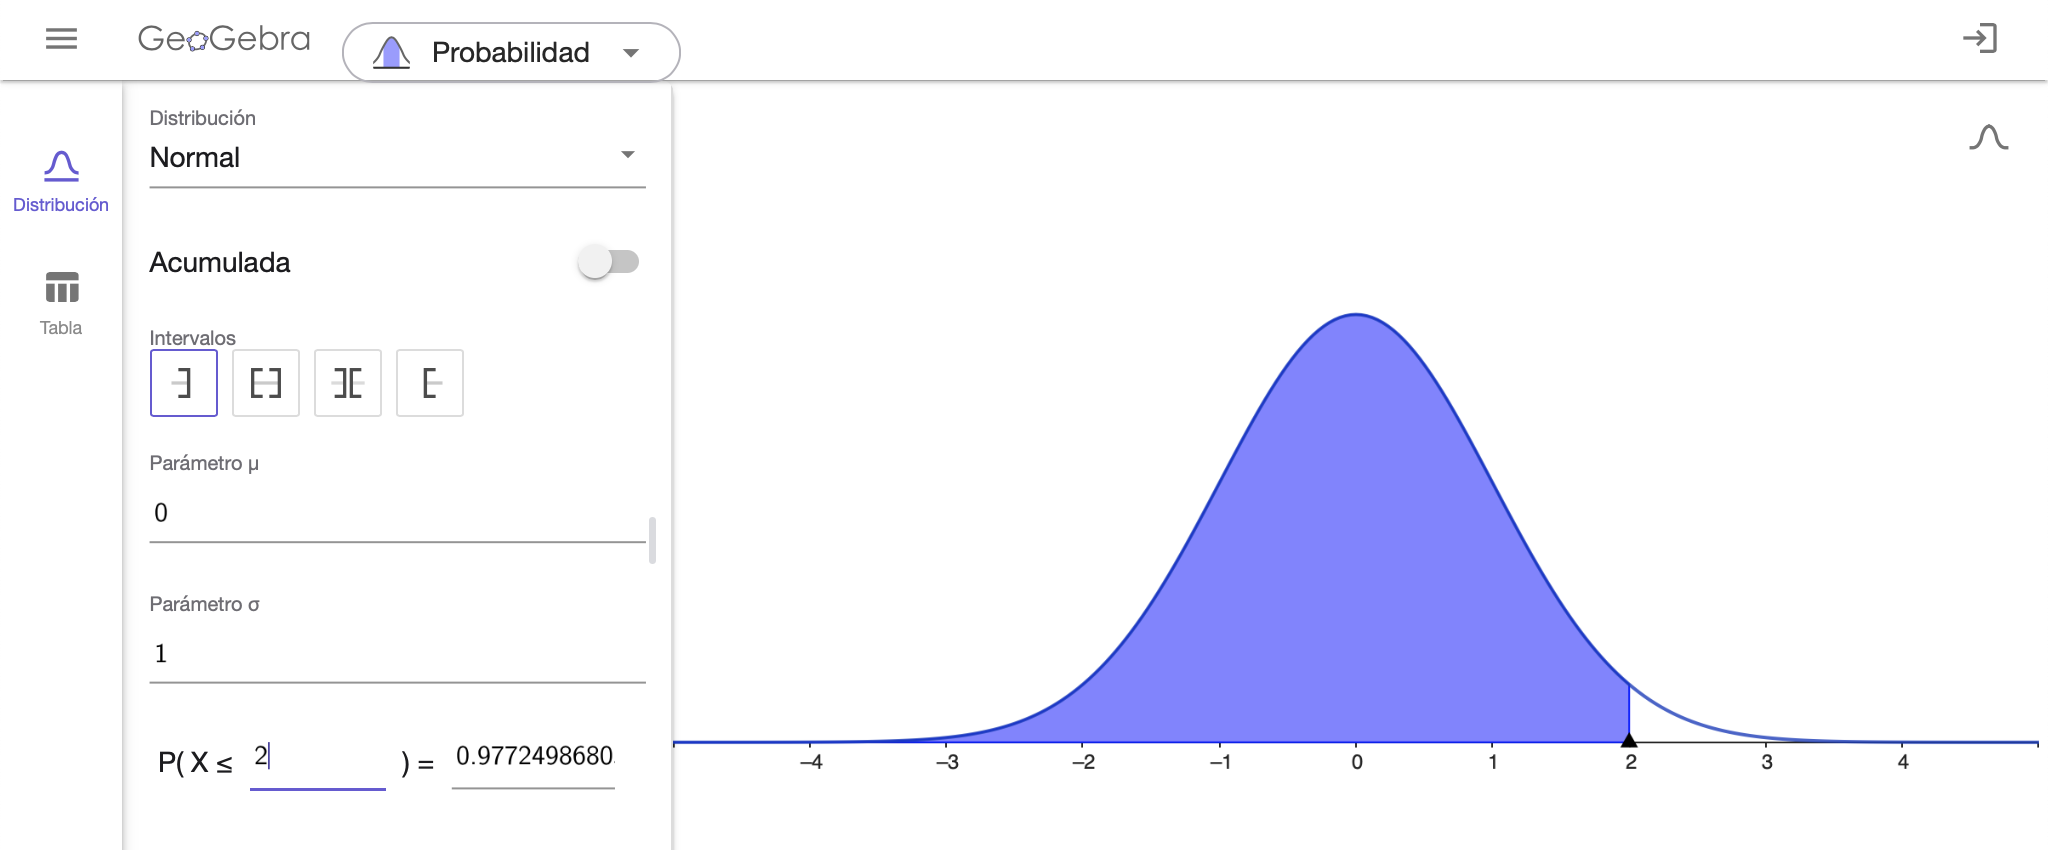
\includegraphics[width=28.44in]{img/3_5}

\textbf{c)} Solución: \(P(-0.5 \leq Z \leq 2.65) = 0.6874\)

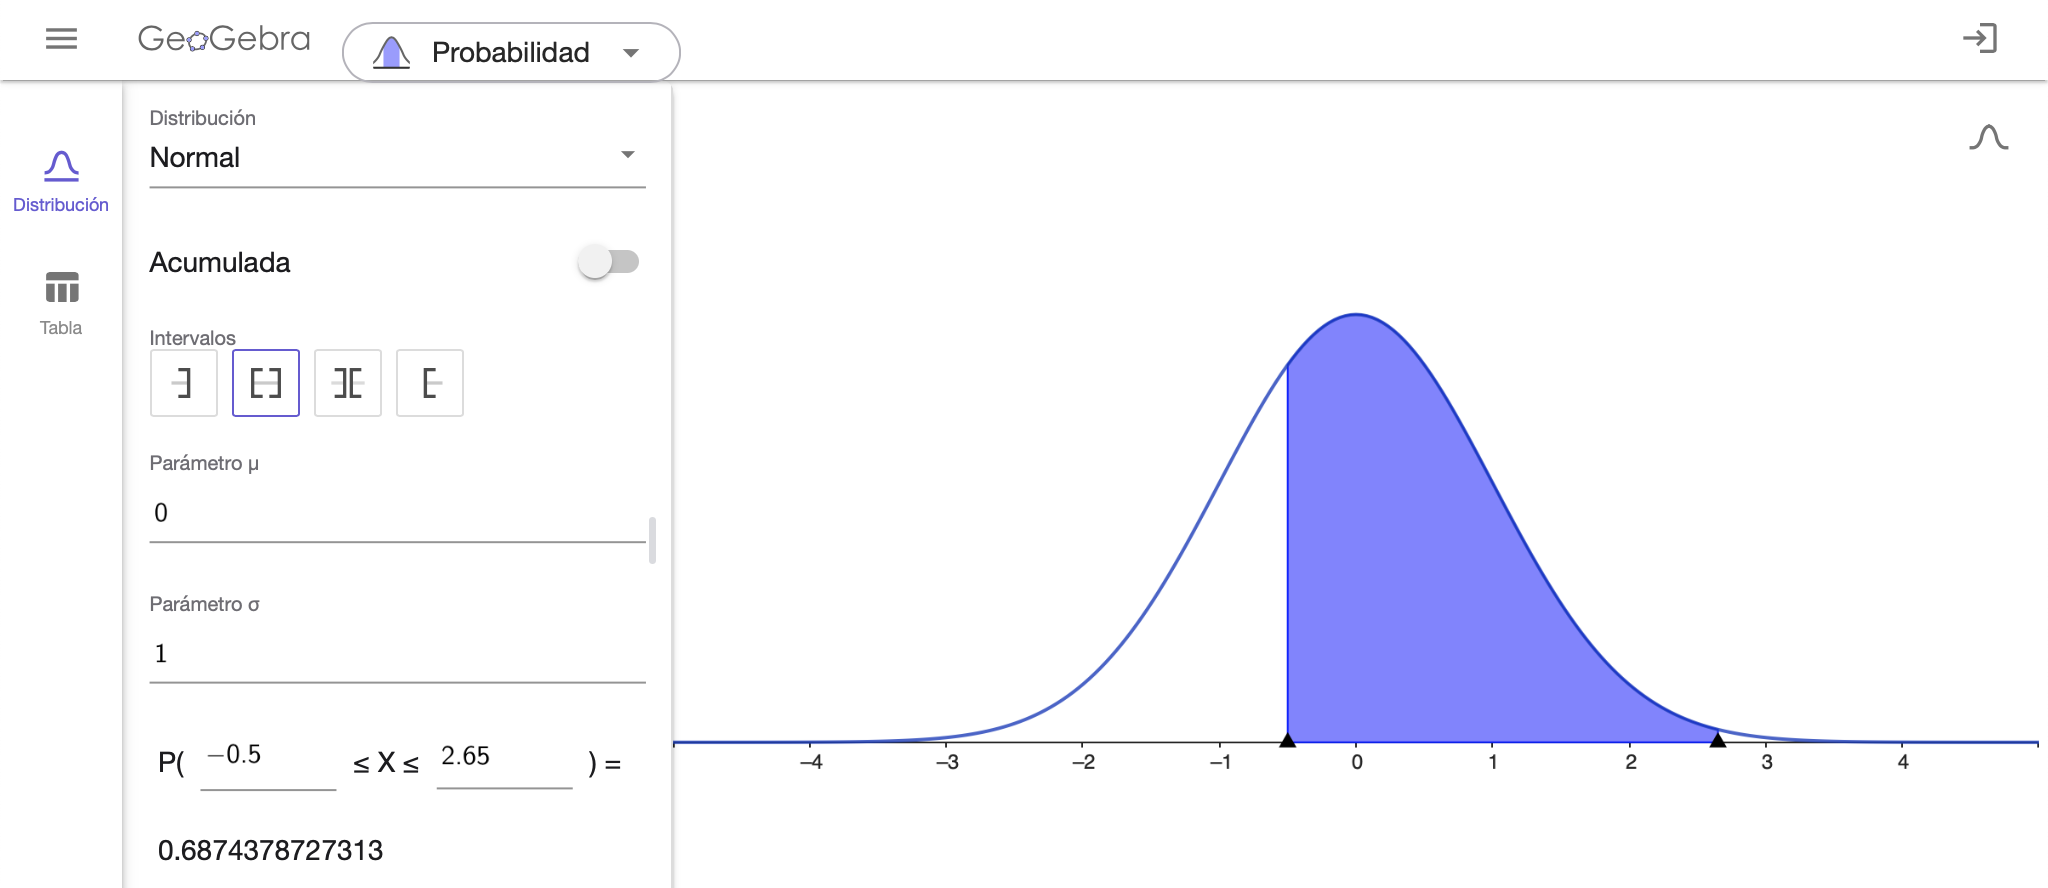
\includegraphics[width=28.44in]{img/3_6}

\textbf{d)} Solución: \(P(0 \leq Z \leq 0.5244) = 0.2\)

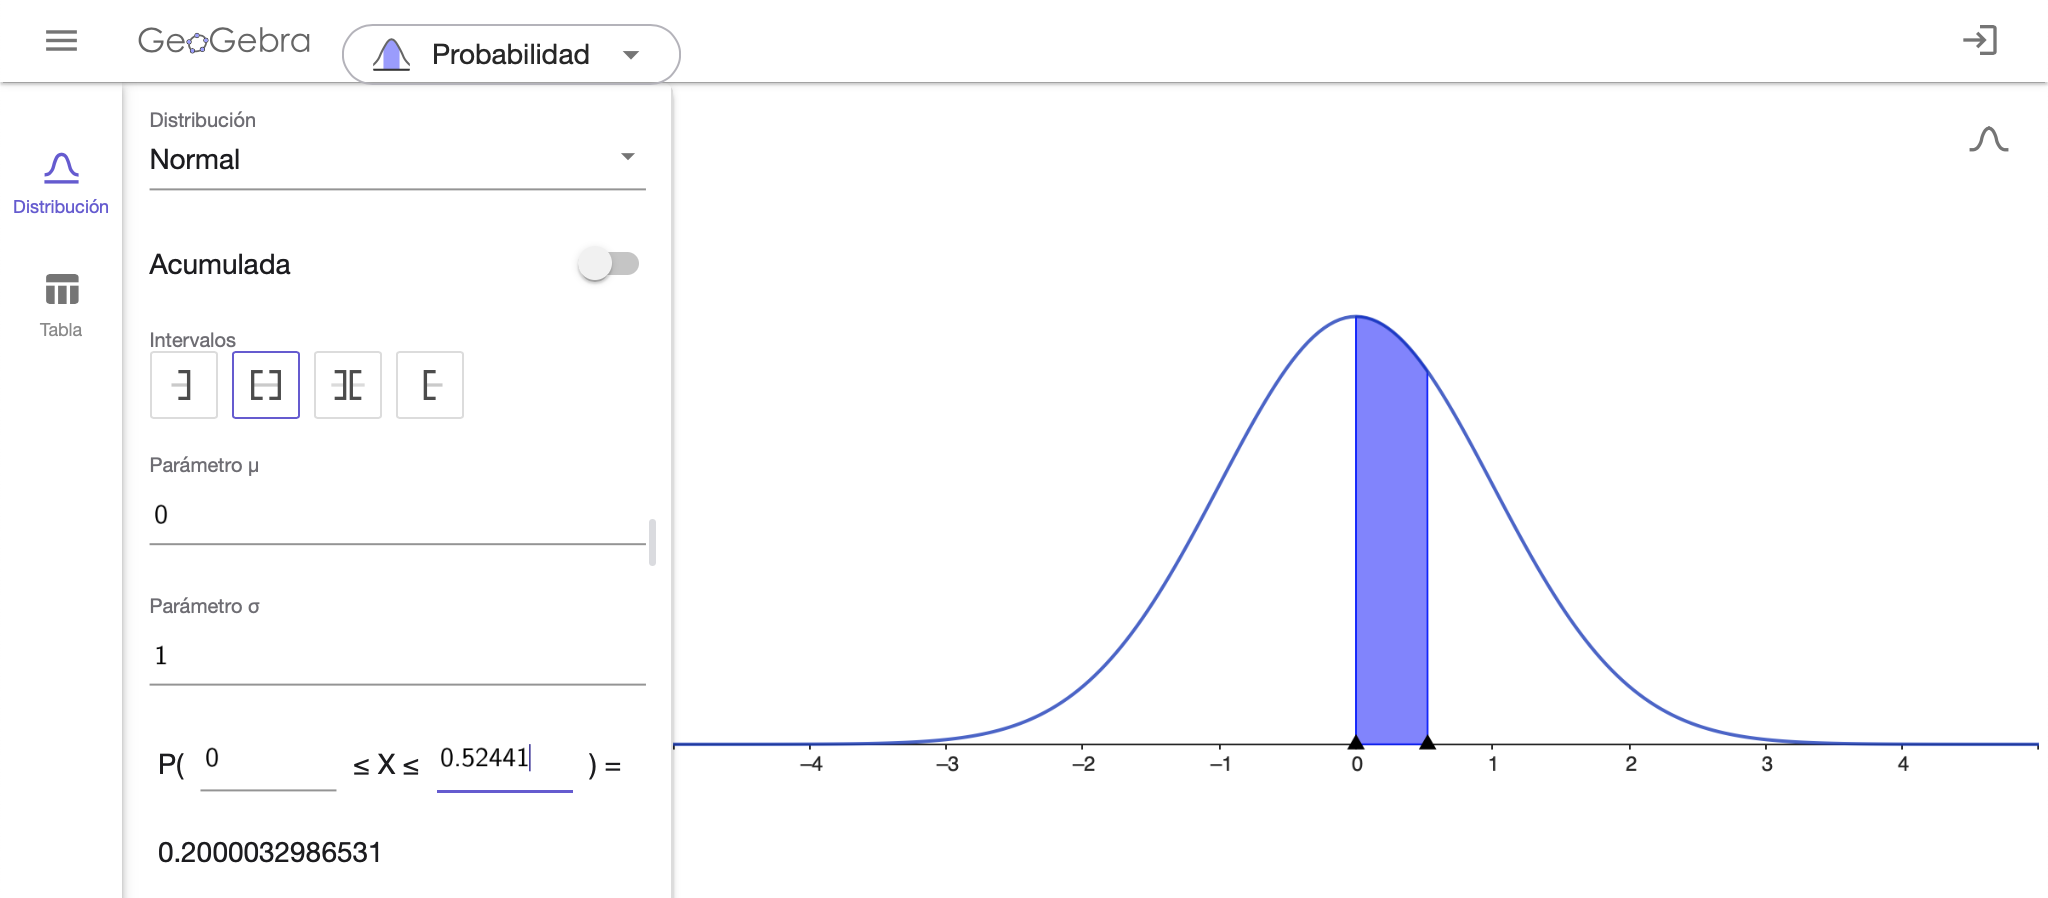
\includegraphics[width=28.44in]{img/3_7}

En este caso, hemos ido aproximando a 4 decimales hasta obtener el valor más próximo a 0.2.

\textbf{e)} Solución: \(P(Z \geq 1.2816) = 0.1\)

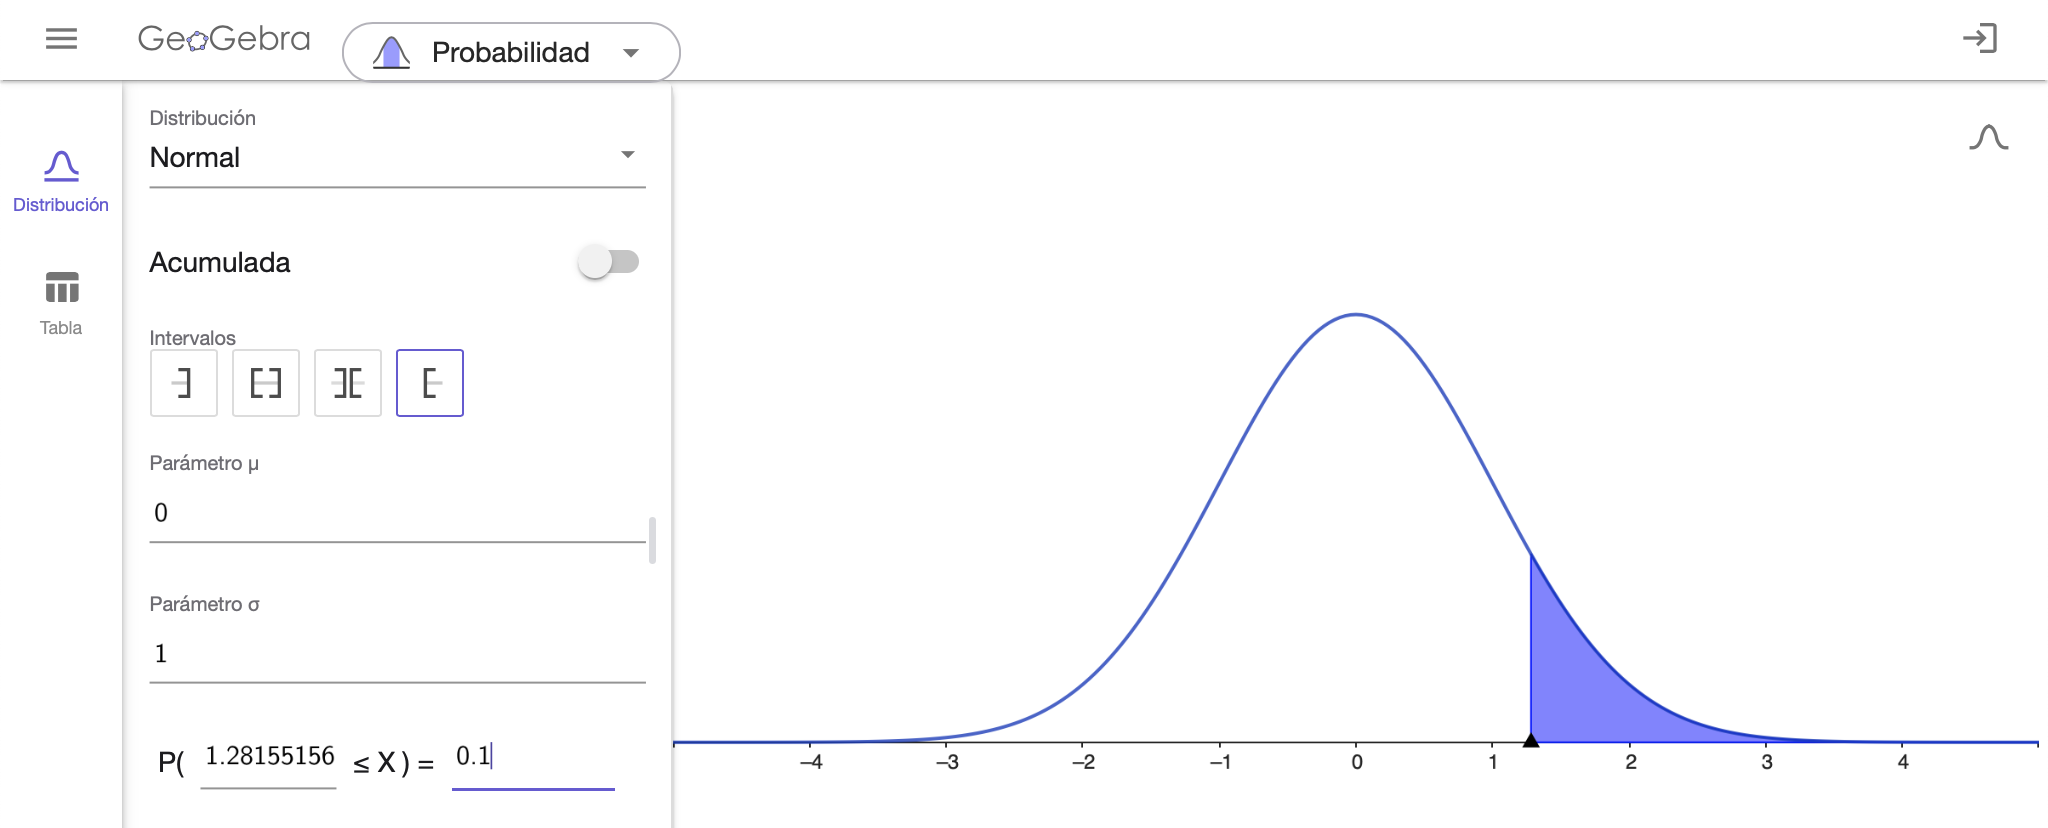
\includegraphics[width=28.44in]{img/3_8}

\hypertarget{pregunta-test-98}{%
\section{Pregunta test}\label{pregunta-test-98}}

Una estimación confidencial para un nivel de confianza fijado, da por respuesta:

\begin{enumerate}
\def\labelenumi{\alph{enumi})}
\tightlist
\item
  Una aproximación de la media.
\item
  Una aproximación de una proporción.
\item
  Una probabilidad.
\item
  Un intervalo.
\item
  Un nivel de significación.
\end{enumerate}

Respuesta correcta

\href{https://1fjmanzano.github.io/bioestadistica/estimacio\%CC\%81n-de-para\%CC\%81metros.-intervalos-de-confianza.html}{Explicación}

\hypertarget{pregunta-test-99}{%
\section{Pregunta test}\label{pregunta-test-99}}

En un contraste de hipótesis la cantidad p es:

\begin{enumerate}
\def\labelenumi{\alph{enumi})}
\tightlist
\item
  Un número pequeño.
\item
  Fijada antes de realizar el contraste.
\item
  La probabilidad de rechazar la hipótesis nula.
\item
  La probabilidad de error al rechazar la hipótesis alternativa.
\item
  Conocida al extraer la muestra y calcular el estadístico experimental.
\end{enumerate}

Respuesta correcta

\href{https://1fjmanzano.github.io/bioestadistica/valor-p.html}{Explicación}

\hypertarget{pregunta-test-100}{%
\section{Pregunta test}\label{pregunta-test-100}}

El perímetro torácico en un grupo de militares presenta distribución gaussiana con 95 cm de media y 5 cm de desviación típica. Elegimos a una muestra de 100 indivíduos y calculamos la media de la misma. Elija la afirmación correcta:

\begin{enumerate}
\def\labelenumi{\alph{enumi})}
\tightlist
\item
  La media de la muestra valdrá 95 cm.
\item
  La media de la muestra sería un valor comprendido entre 90 y 100 cm con confianza del 68\%.
\item
  La media de la muestra será un valor comprendido entre 95 y 100 cm con confianza del 95\%.
\item
  La media de la muestra será un valor comprendido entre 94 y 96 cm con confianza del 95\%.
\item
  Todo lo anterior es falso.
\end{enumerate}

Respuesta correcta

\textbf{Explicación}

Consideramos la variable aleatoria

\(X\) = perímetro torácico en un grupo de militares \(X \equiv N(95, 5)\)

El intervalo de confianza para la media muestral \(\overline{x}\) al 95\% será:

\(\mu \pm z_{\alpha/2} \cdot \frac{\sigma}{\sqrt{n}}\)

Para una confianza del 95\%, \(z_{\alpha/2} = 1.96\) (\href{https://youtu.be/wWeogWp_bO8}{ver vídeo}) de donde:

\(\mu \pm z_{\alpha/2} \cdot \frac{\sigma}{\sqrt{n}}= 95 = 95 \pm 1.95 \cdot \frac{5}{\sqrt{100}}= (94.02002,95.97998) \approx (94, 96)\)

Se puede comprobar el resultado utilizando el applet \href{https://homepage.divms.uiowa.edu/~mbognar/applets/mu.raw.html}{Probability Distributios: Statistical Inference for \(\mu\)} introduciendo los valores \(n=100\), \(\overline{x}=95\) y \(\sigma = 5\) con \(95\) \% de CI (confidence Interval) y activando la opción \emph{Show equations}.

\hypertarget{pregunta-test-101}{%
\section{Pregunta test}\label{pregunta-test-101}}

El consumo diario de Calorías se distribuye en una población de forma normal, con media 2500 y desviación típica 100. Si elijo una muestra de tamaño 100, entre qué valores espero encontrar su media (con una probabilidad del 95\% de acertar):

\begin{enumerate}
\def\labelenumi{\alph{enumi})}
\tightlist
\item
  Entre 2400 y 2600.
\item
  Entre 2300 y 2700.
\item
  Entre 2490 y 2510.
\item
  Entre 2480 y 2520.
\item
  Entre 2498 y 2502.
\end{enumerate}

Respuesta correcta

\href{https://homepage.divms.uiowa.edu/~mbognar/}{Explicación}

\hypertarget{problema-12}{%
\section{Problema}\label{problema-12}}

El nivel de colesterol en la sangre se mide de acuerdo a un índice llamado LDL. Para el caso de personas adultas, la distribución del colesterol en la sangre es aproximadamente normal y en el caso de los hombres tiene una media de \(4.8\) unidades LDL con una desviación estándar igual a \(0.6\) unidades. El nivel normal (o riesgo normal) de colesterol se considera aquel que queda entre los límites \(\mu \pm \sigma\) en unidades LDL. Una persona con más de \(\mu + \sigma\) pero menos de \$\mu + 2\sigma \$ unidades LDL tiene un nivel de riesgo moderado. Si tiene un nivel de \$\mu + 2\sigma \$ o superior se considera de alto riesgo y se hace propenso a sufrir un infarto. Por otra parte, si el nivel de colesterol en la sangre de un adulto está por debajo de \(\mu - \sigma\) unidades, se considera de riesgo bajo.

\textbf{a)} ¿Cuáles son los porcentajes de población de hombres adultos que están incluidos en cada uno de los 4 niveles de riesgo descritos?

\textbf{b)} ¿A partir de qué nivel de colesterol se encuentra el 10 \% de la población de hombres adultos con mayor riesgo?

\textbf{a)} Los niveles son:

\begin{longtable}[]{@{}cc@{}}
\toprule
Riesgo & Nivel de LDL\tabularnewline
\midrule
\endhead
Bajo & \(< 4.2\)\tabularnewline
Normal & \(4.2 -5.4\)\tabularnewline
Moderado & \(5.4 -6\)\tabularnewline
Alto & \(> 6\)\tabularnewline
\bottomrule
\end{longtable}

Utilizando la \href{https://www.geogebra.org/calculator}{calculadora de Probabilidad de Geogebra} obtenemos los porcentajes de poblacion:

\begin{longtable}[]{@{}ccc@{}}
\toprule
Riesgo & Nivel de LDL & \% población\tabularnewline
\midrule
\endhead
Bajo & \(< 4.2\) & \(15.9 \%\)\tabularnewline
Normal & \(4.2 - 5.4\) & \(68.3 \%\)\tabularnewline
Moderado & \(5.4 - 6\) & \(13.6 \%\)\tabularnewline
Alto & \(> 6\) & \(2.2 \%\)\tabularnewline
\bottomrule
\end{longtable}

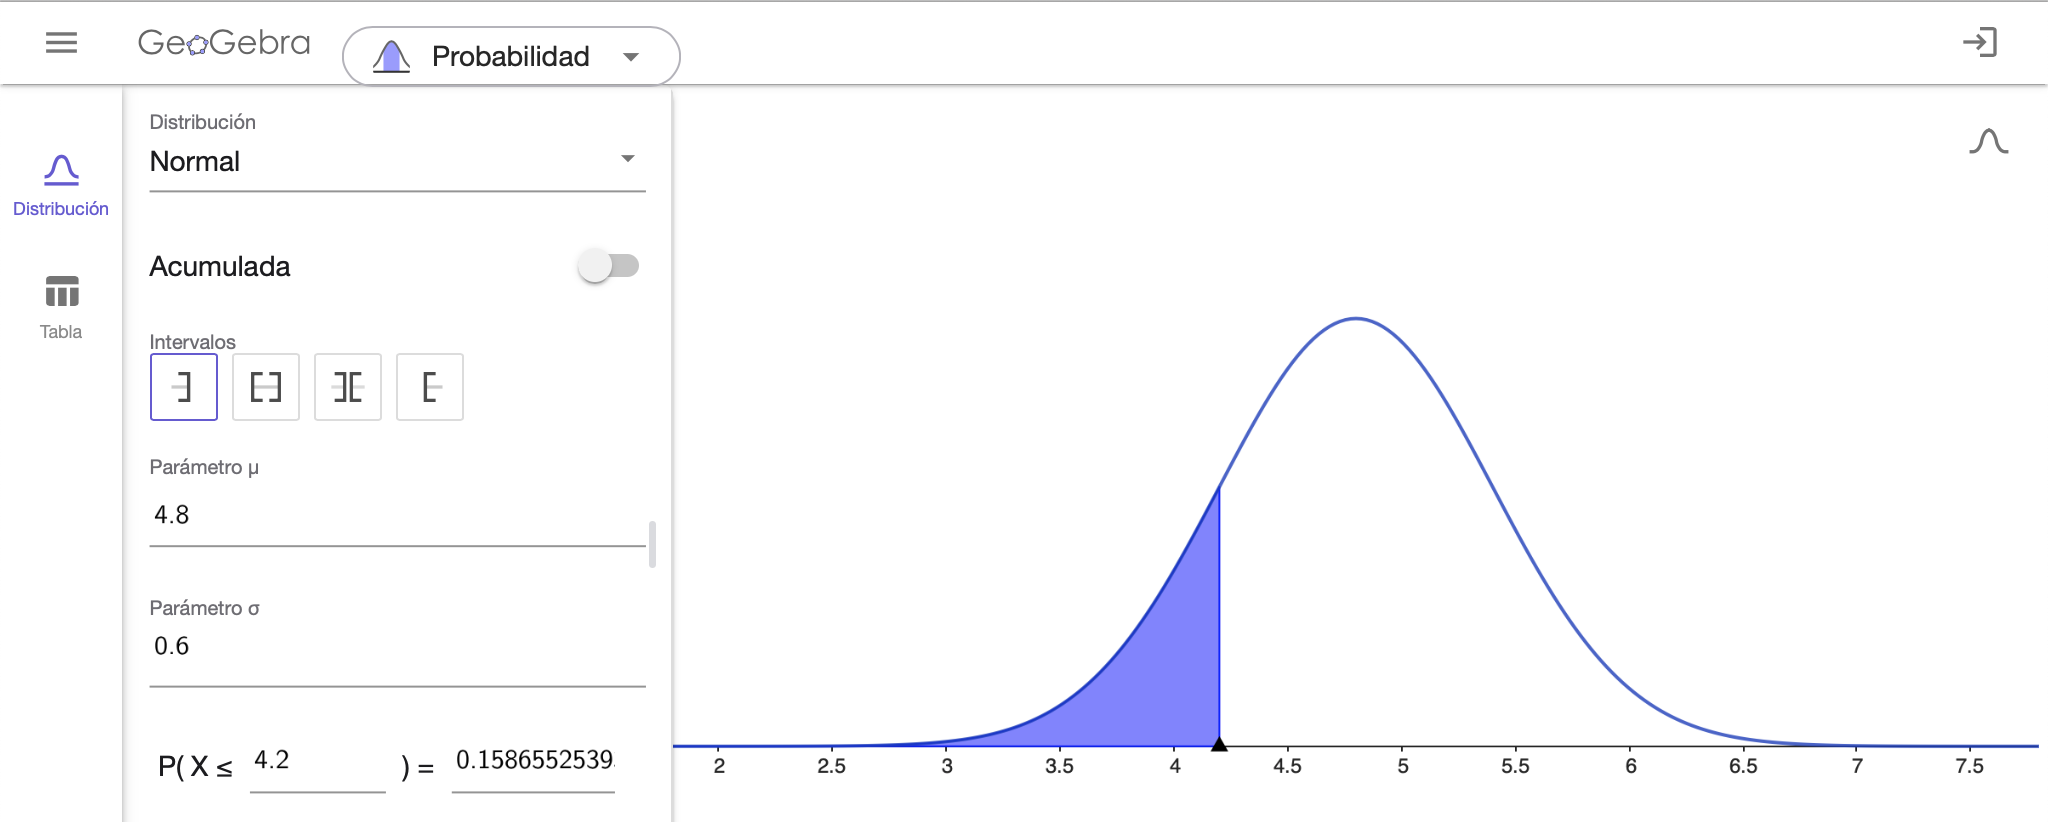
\includegraphics[width=28.44in]{img/3_9}

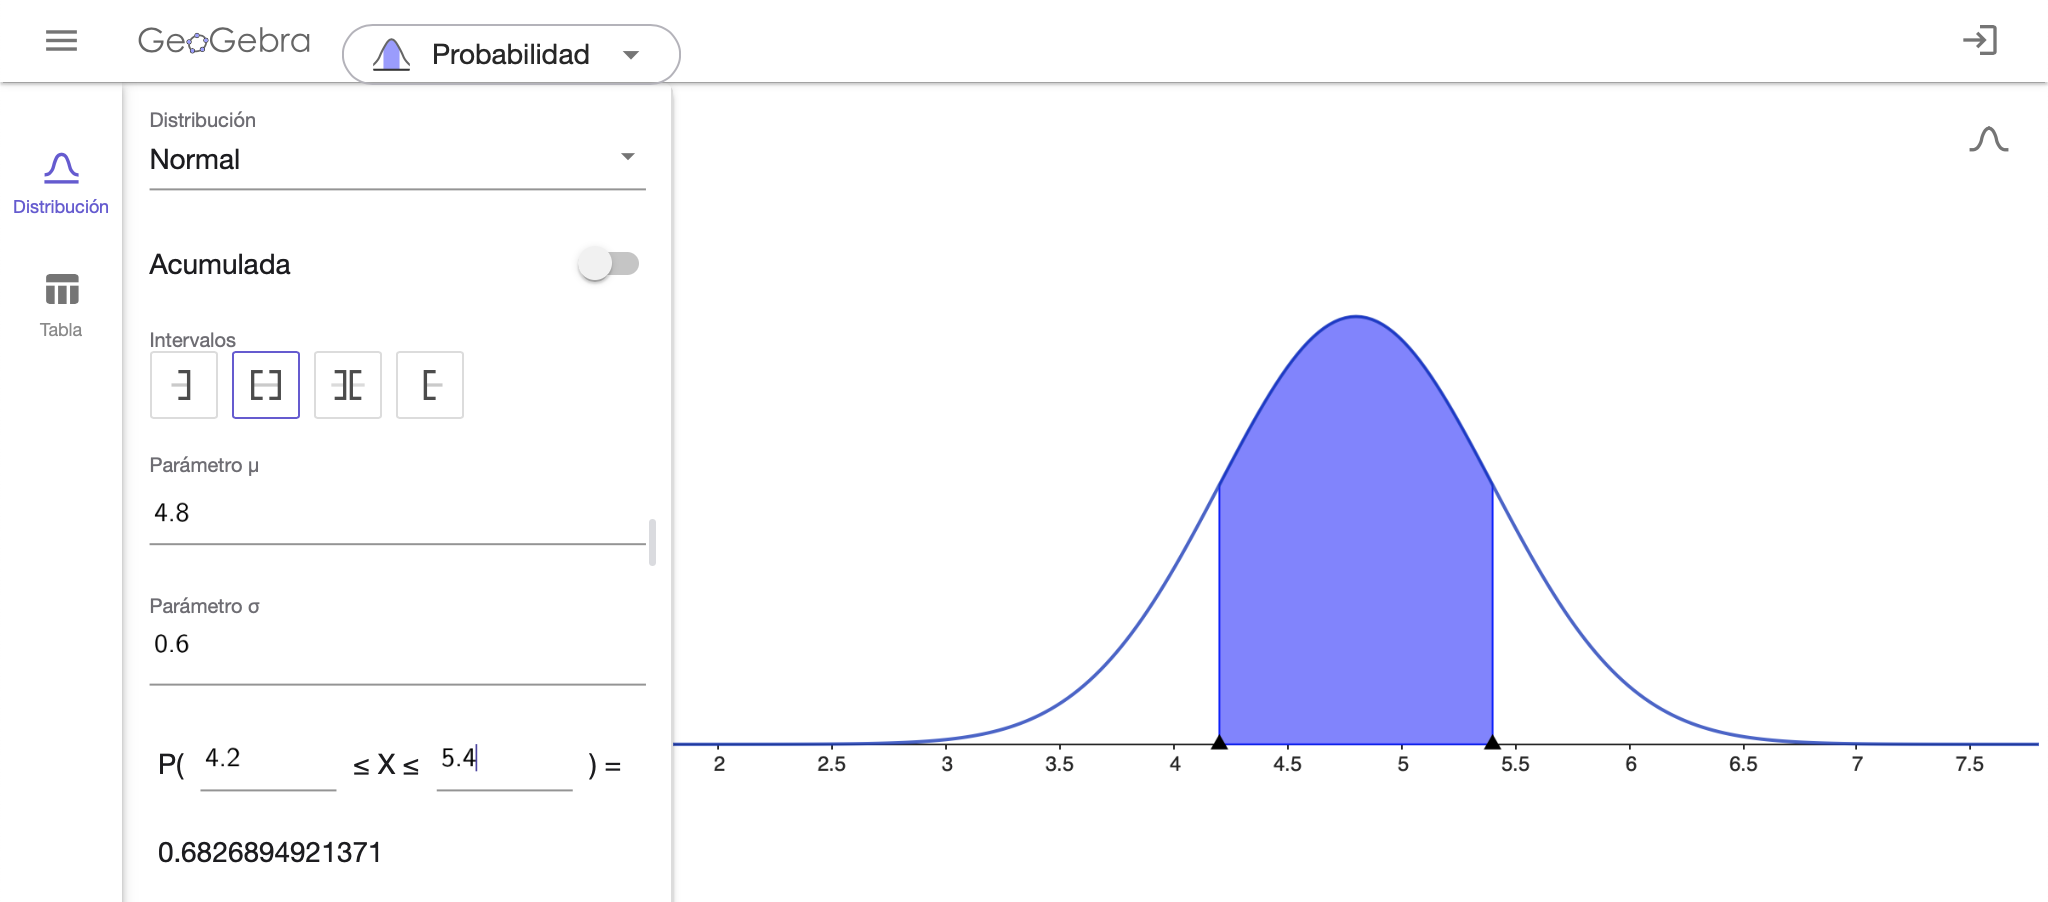
\includegraphics[width=28.44in]{img/3_10}

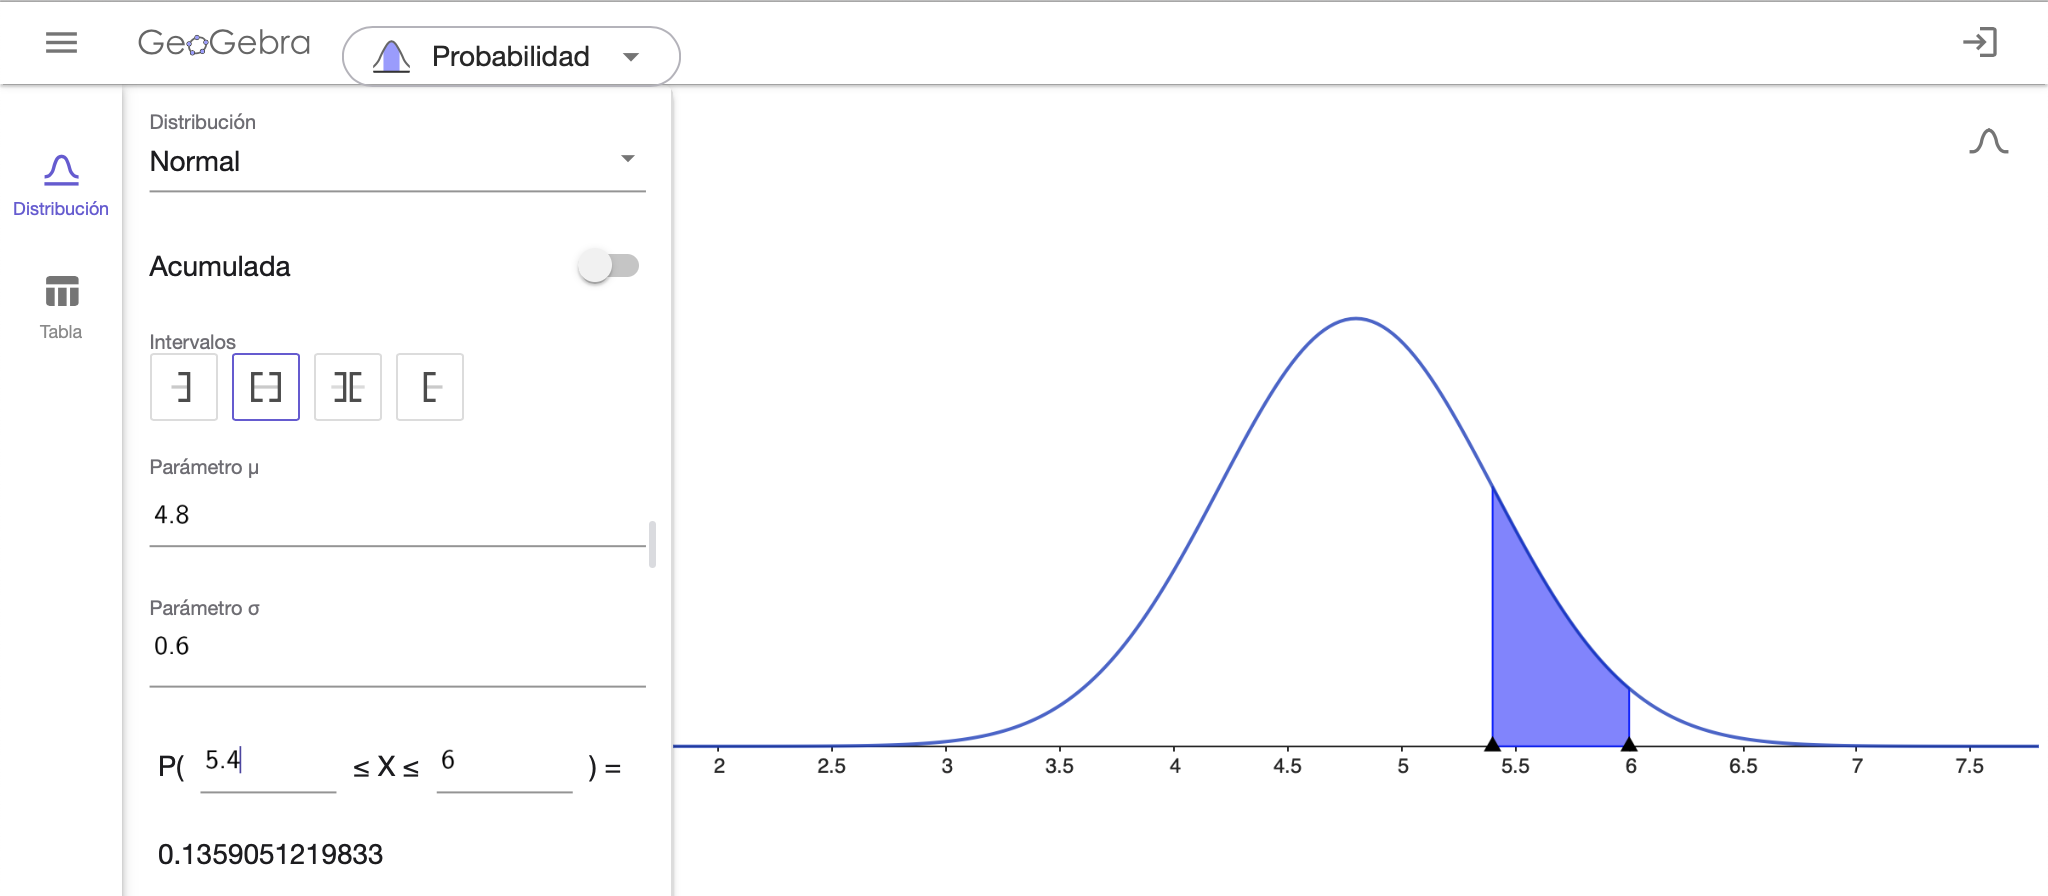
\includegraphics[width=28.44in]{img/3_11}

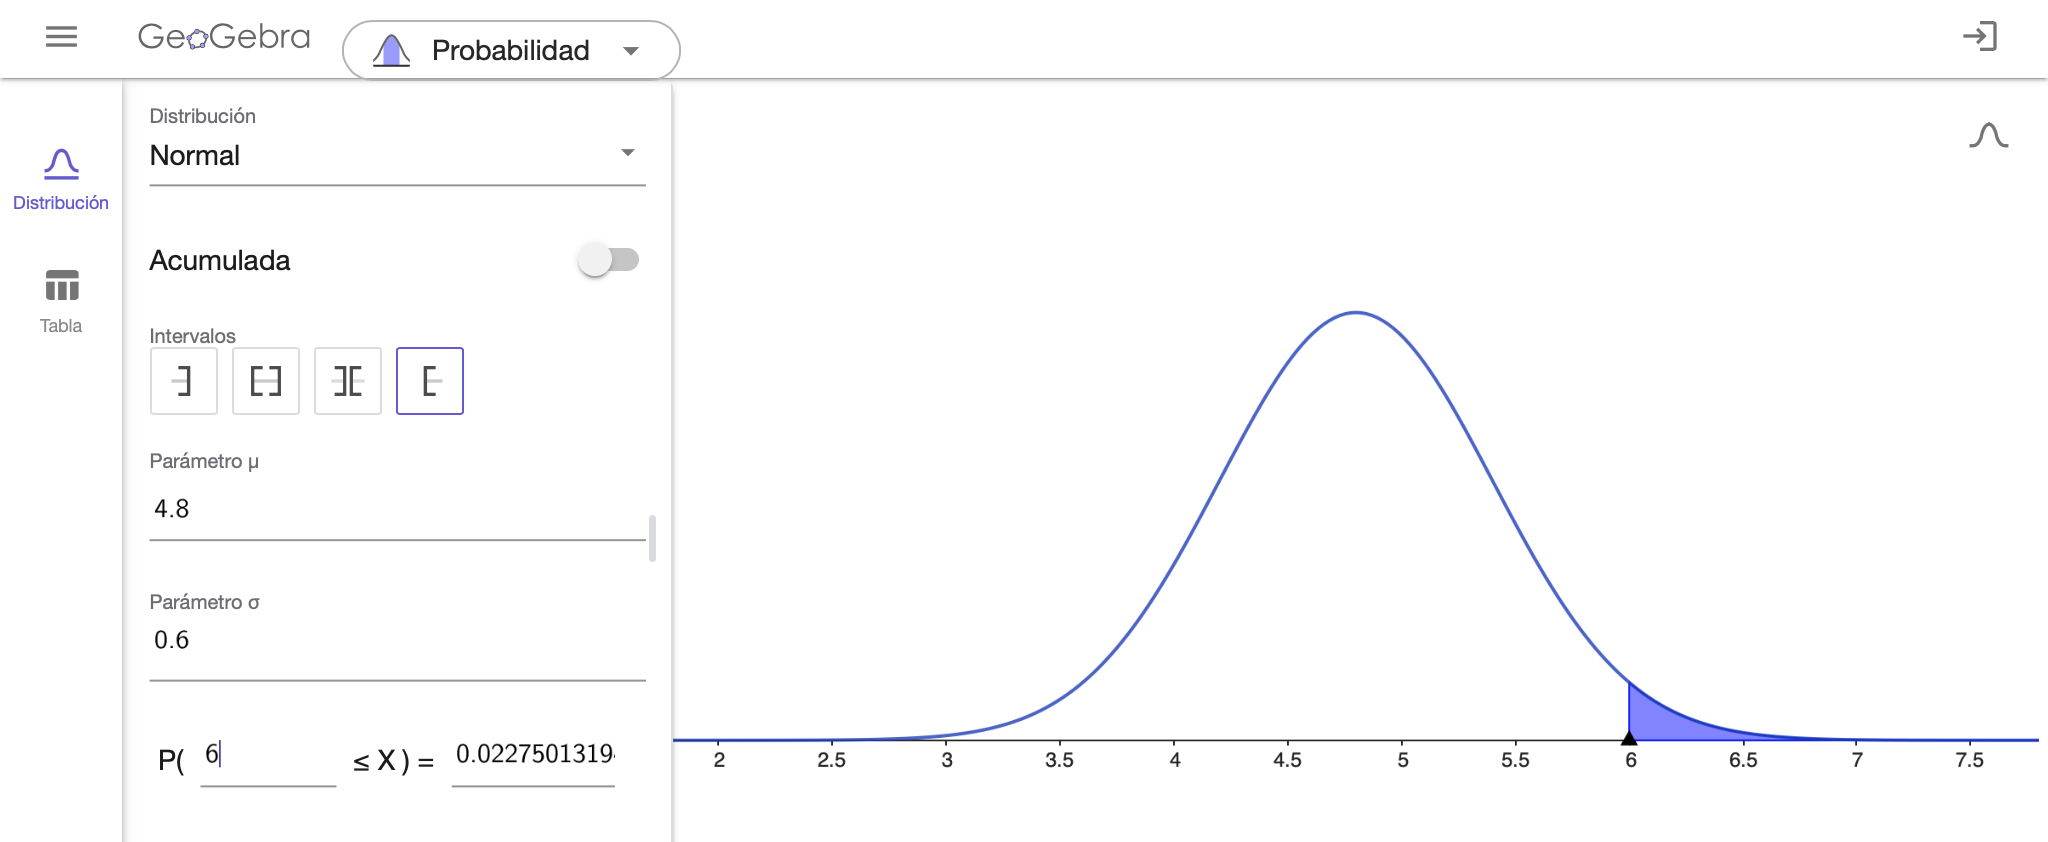
\includegraphics[width=28.44in]{img/3_12}

\textbf{b)} Siendo \(X\) = nivel de colesterol en la sangre, tenemos que calcular el valor de \(x\) para el que \(P(X > x) = 0.10\) (normal inversa). Con Geogebra, obtenemos que ese valor es \(5.57\).

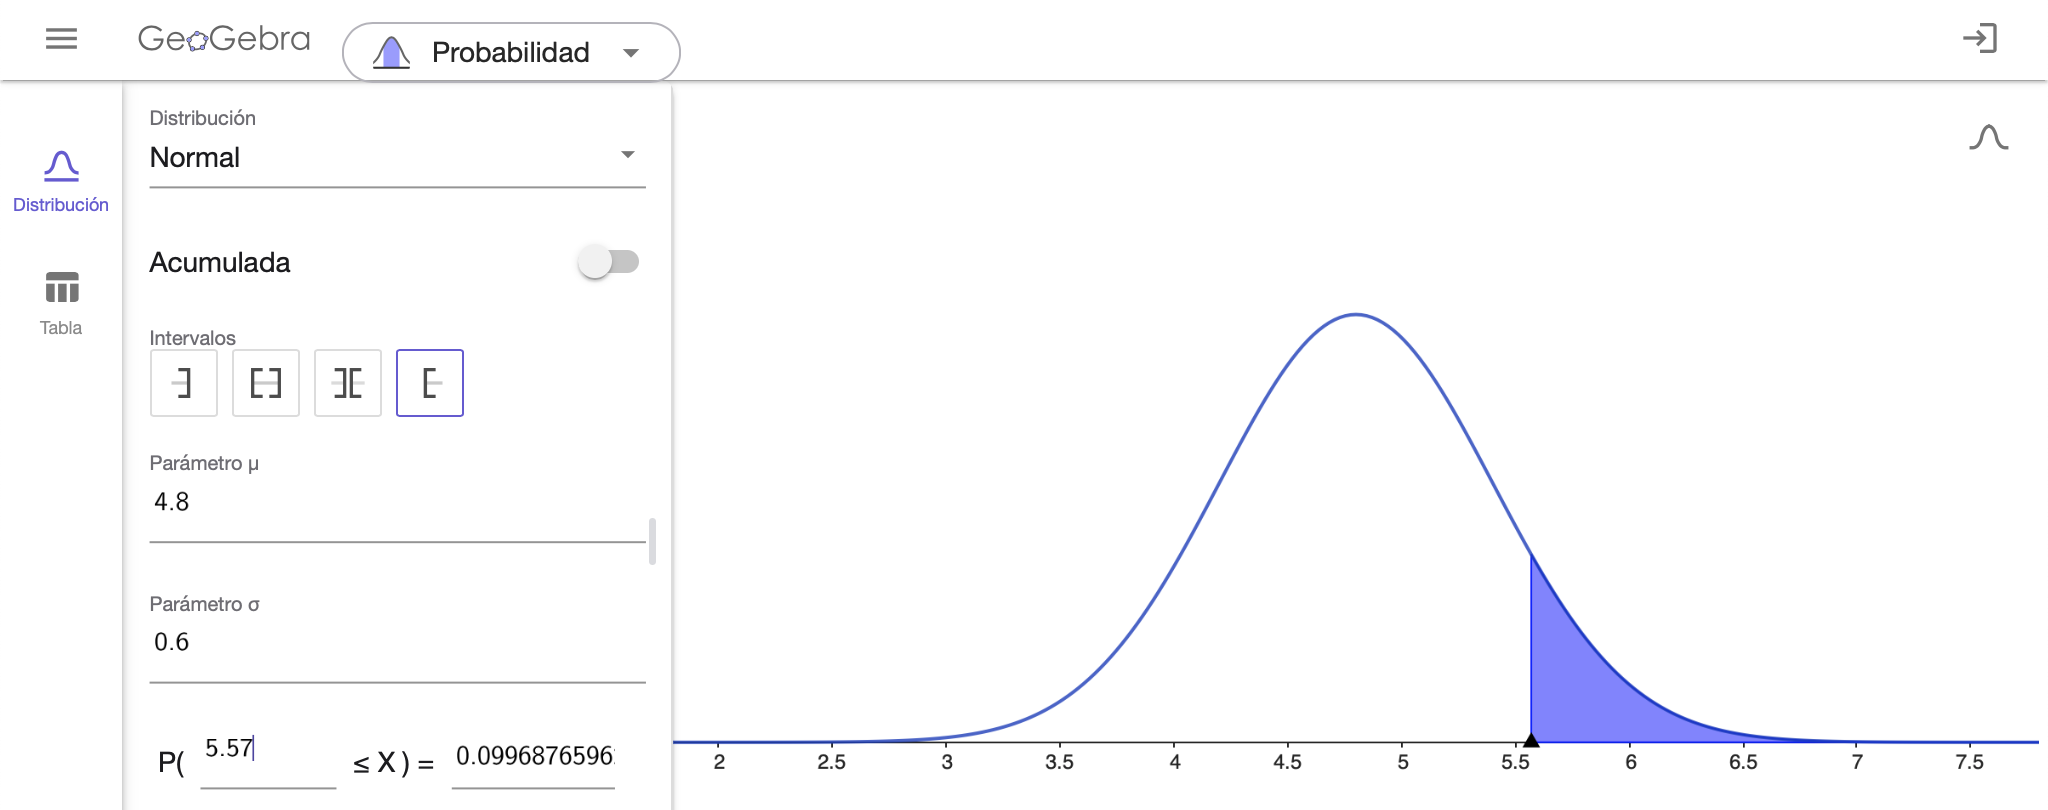
\includegraphics[width=28.44in]{img/3_13}

\hypertarget{pregunta-test-102}{%
\section{Pregunta test}\label{pregunta-test-102}}

Un contraste de hipótesis se considera significativo si:

\begin{enumerate}
\def\labelenumi{\alph{enumi})}
\tightlist
\item
  Una muestra aleatoria es coherente con la hipótesis nula.
\item
  Una muestra aleatoria no es coherente con la hipótesis nula.
\item
  La hipótesis alternativa es más probable que la nula.
\item
  Todo lo anterior es cierto.
\item
  Son ciertas (b) y (c).
\end{enumerate}

Respuesta correcta

\href{https://1fjmanzano.github.io/bioestadistica/contrastes-de-hipo\%CC\%81tesis.html}{Explicación}

\hypertarget{pregunta-test-103}{%
\section{Pregunta test}\label{pregunta-test-103}}

En una muestra aleatoria de 100 individuos se obtiene una media muestral de 50, la desviación típica es 20. Elija la afirmación correcta:

\begin{enumerate}
\def\labelenumi{\alph{enumi})}
\tightlist
\item
  El 68\% de los individuos de la muestra tiene sus valores comprendidos entre 48 y 52.
\item
  El 95\% de los individuos de la muestra tiene sus valores comprendidos entre 46 y 54.
\item
  Hay una probabilidad del 68\% de que la media de la población esté comprendida entre 30 y 70.
\item
  Hay una probabilidad del 95\% de que la media de la población esté entre 46 y 54.
\item
  Todo lo anterior es falso.
\end{enumerate}

Respuesta correcta

\href{https://homepage.divms.uiowa.edu/~mbognar/}{Explicación}

\hypertarget{pregunta-test-104}{%
\section{Pregunta test}\label{pregunta-test-104}}

Un contraste de hipótesis se considera no significativo si:

\begin{enumerate}
\def\labelenumi{\alph{enumi})}
\tightlist
\item
  Una muestra aleatoria es coherente con la hipótesis nula.
\item
  Una muestra aleatoria no es coherente con la hipótesis nula.
\item
  La hipótesis nula es más probable que la alternativa.
\item
  Todo lo anterior es cierto.
\item
  Son ciertas (a) y (c).
\end{enumerate}

Respuesta correcta

\href{https://1fjmanzano.github.io/bioestadistica/contrastes-de-hipo\%CC\%81tesis.html}{Explicación}

\hypertarget{pregunta-test-105}{%
\section{Pregunta test}\label{pregunta-test-105}}

Una muestra aleatoria de 64 pacientes refleja que el presión arterial diastólica media es 150 (DT 16), con distribución aproximadamente normal. Elija la afirmación correcta.

\begin{enumerate}
\def\labelenumi{\alph{enumi})}
\tightlist
\item
  La media de la población está con confianza del 95\% entre 134 y 166
\item
  La media de la población está con confianza del 68\% entre 142 y 158
\item
  La media de la población está con confianza del 95\% entre 148 y 152
\item
  La media de la población está con confianza del 95\% entre 146 y 154
\item
  El error típico es de 1 punto.
\end{enumerate}

Respuesta correcta

\href{https://homepage.divms.uiowa.edu/~mbognar/}{Explicación}

\hypertarget{problema-13}{%
\section{Problema}\label{problema-13}}

Para ayudar a la evaluación del pronóstico de pacientes con una determinada enfermedad pulmonar se calculan dos índices, independientes entre sí. Se asume que el primero de los índices se distribuye según una normal \(N(120,10)\) y que el segundo se distribuye según una normal \(N(15,3)\). Se consideran susceptibles de una revisión más profunda aquellos pacientes que en el primer índice superen el valor 142. También son susceptibles de una revisión más profunda aquellos pacientes que en el segundo índice presenten un valor inferior a 8. ¿Qué porcentaje de pacientes son susceptibles de una revisión más profunda?

\hypertarget{soluciuxf3n-10}{%
\subsection{Solución}\label{soluciuxf3n-10}}

Definimos los sucesos y calculamos sus probabilidades con \href{https://homepage.divms.uiowa.edu/~mbognar/applets/normal.html}{Probability Distributions: Normal Distribution}:

\begin{itemize}
\tightlist
\item
  \(A\) = valor superior a 142 en el primer índice \(P(A)=0.0139\)
\item
  \(B\) = valor inferior a 8 en el segundo índice \(P(B)=0.00982\)
\end{itemize}

De este modo, los pacientes susceptible de una revisión más profunda serán los del suceso \(A \cup B\).

Sabemos que \(P(A \cup B)= P(A) + P(B) - P(A \cap B)\). Así, nos falta saber el valor de \(P(A \cap B)\) (probabilidad de ser susceptible de una revisión más profunda por los 2 índices).

Nos dicen que los índices son independientes. Entonces

\(P(A \cap B) = P(A) \cdot P(B) = 0.0139 \cdot 0.00982 = 0.000136498\), probabilidad prácticamente nula.

Así, \(P(A \cup B)= P(A) + P(B) - P(A \cap B) = 0.0139 + 00982 - 0.000136498 = 0.0235835\).

Entonces, \textbf{́el 2.36 \% de pacientes son susceptibles de una revisión más profunda}

\hypertarget{pregunta-test-106}{%
\section{Pregunta test}\label{pregunta-test-106}}

Qúe propiedad o propiedades caracterizan a una distribución normal tipificada frente a una distribución normal cualquiera:

\begin{enumerate}
\def\labelenumi{\alph{enumi})}
\tightlist
\item
  El área bajo su función de densidad es igual a 1.
\item
  Su media es 1 y su desviación típica es 0.
\item
  Su rango de valores oscila entre 0 y 3.
\item
  Su media es 0 y su desviación típica es 1.
\item
  Son ciertas (c) y (d)
\end{enumerate}

Respuesta correcta

\href{https://1fjmanzano.github.io/bioestadistica/distribuciones-de-probabilidad.html\#distribucio\%CC\%81n-z}{Explicación}

\hypertarget{pregunta-test-107}{%
\section{Pregunta test}\label{pregunta-test-107}}

En relación con los contrastes de hipótesis, elija la afirmación correcta:

\begin{enumerate}
\def\labelenumi{\alph{enumi})}
\tightlist
\item
  La hipótesis nula es la correcta.
\item
  La hipótesis nula es la falsa.
\item
  Si la hipótesis alternativa es cierta, seguro que se rechaza la nula.
\item
  El contraste es significativo cuando los datos muestrales no son los esperados si la hipótesis nula fuese cierta,
\item
  Si es más probable que sea cierta la hipótesis alternativa que la nula, el contraste es significativo.
\end{enumerate}

Respuesta correcta

\href{https://1fjmanzano.github.io/bioestadistica/contrastes-de-hipo\%CC\%81tesis.html}{Explicación}

\hypertarget{pregunta-test-108}{%
\section{Pregunta test}\label{pregunta-test-108}}

En una población, el peso tiene media 60 kg y desviación típica 6 Kg. La altura tiene de media 170 cm y desviación 6 cm. Cierto individuo tiene un peso de 70 Kg y altura 180 cm.

\begin{enumerate}
\def\labelenumi{\alph{enumi})}
\tightlist
\item
  La altura tiene un valor más extremo que el peso.
\item
  El peso es menos extremo que la altura.
\item
  Peso y altura son valores igualmente extremos.
\item
  El peso es más extremo que la altura.
\item
  La altura es menos extrema que el peso.
\end{enumerate}

Respuesta correcta

\textbf{Explicación}

En este caso debemos comparar valores en 2 variables normales (o gaussianas):

\begin{itemize}
\tightlist
\item
  Peso \(\equiv N(60, 6)\) para un valor de 70 kg.
\item
  Altura \(\equiv N(170, 6)\) para un valor de 180 cm.
\end{itemize}

Podemos hacerlo con una tabla (\href{https://youtu.be/xCBUdpIUx18}{ver vídeo}) o usando Excel@ o una app específica. (\href{https://youtu.be/rxkPlU1Ud7c}{ver vídeo}).

Utilizando la aplicación \href{https://homepage.divms.uiowa.edu/~mbognar/applets/normal.html}{Probability Distributions: Normal Distribution}, obtenemos la probabilidad de pesar menos de 70 kg:

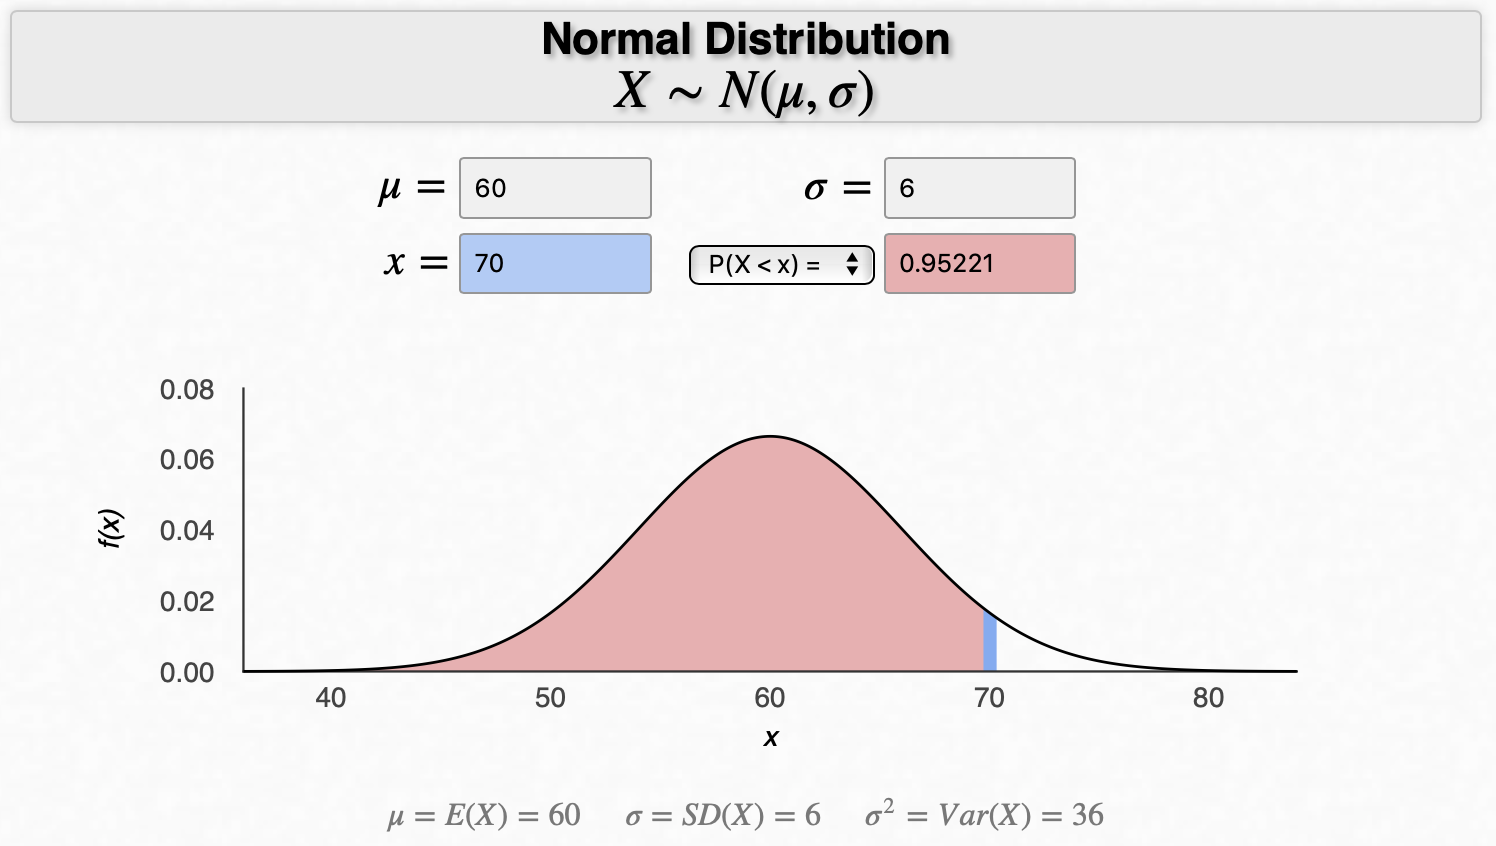
\includegraphics[width=20.78in]{img/3_1}

y la probabilidad de medir menos de 180 cm:

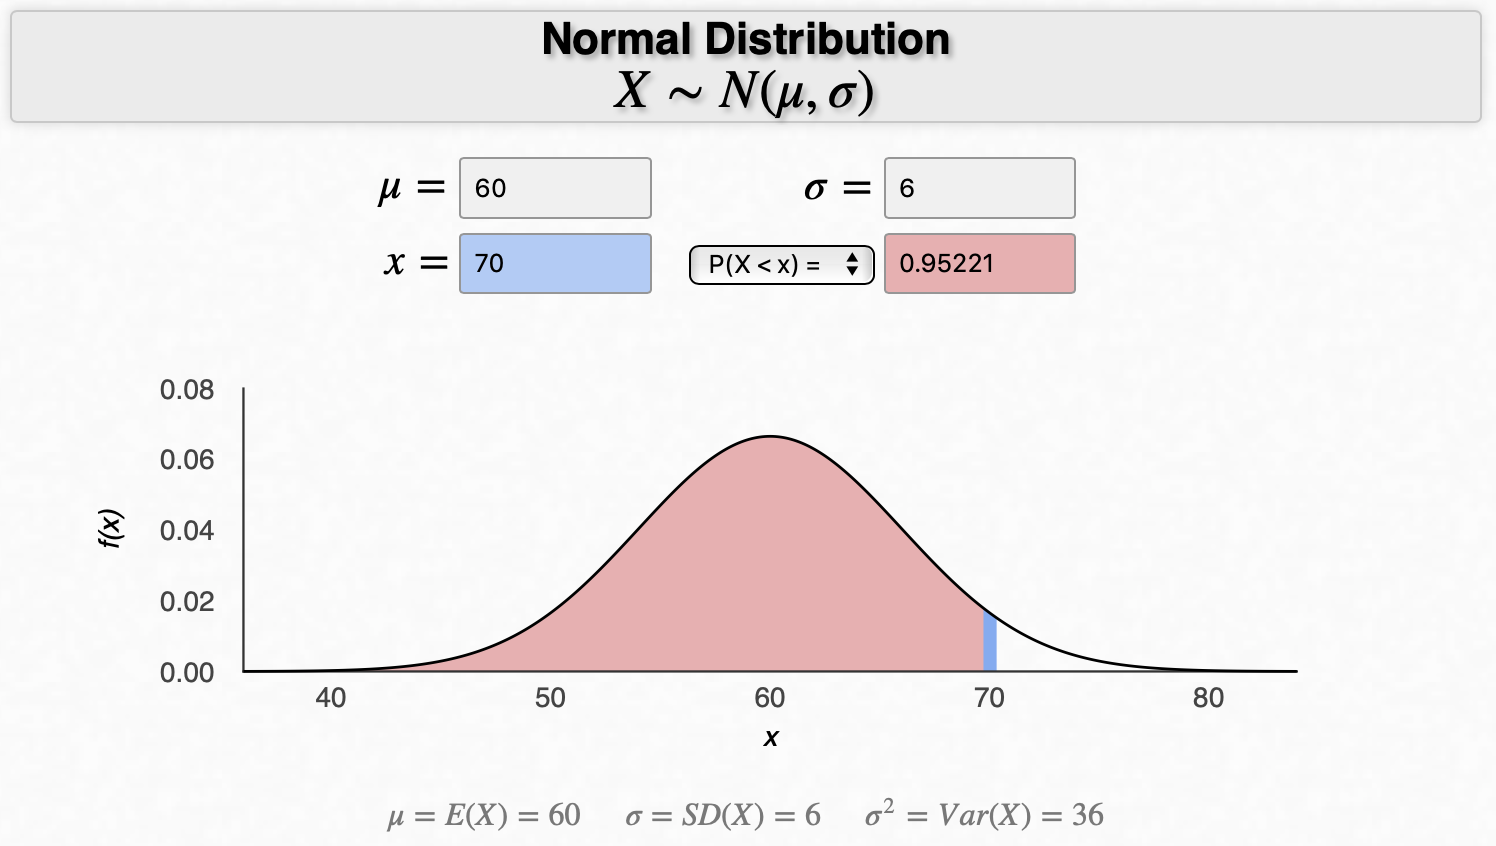
\includegraphics[width=20.78in]{img/3_1}

En ambos casos, la probabilidad es \(0.95221\)

\hypertarget{pregunta-test-109}{%
\section{Pregunta test}\label{pregunta-test-109}}

El nivel medio de glucemia en una población tiene un comportamiento gausiano con media 150mg/dl, y un coeficiente de variación del 10\%. Entre qué valores se situa el 95\% de los individuos de la población.

\begin{enumerate}
\def\labelenumi{\alph{enumi})}
\tightlist
\item
  Entre 140 y 160.
\item
  Entre 130 y 170.
\item
  Entre 120 y 180.
\item
  Entre 110 y 190.
\item
  Entre 100 y 200.
\end{enumerate}

Respuesta correcta

\textbf{Explicación}

En este caso, nos dan el coeficiente de variación, \(CV=\frac{\sigma}{\overline{x}}\). Entonces:

\(0.10 = \frac{\sigma}{150} \Rightarrow \sigma = 15\)

Así la variable \(X\) = nivel medio de glucemia \(\equiv N(150, 15)\).

En una distribución normal, el 95\% de los datos están en el intervalo \(\mu \pm 2 \sigma= 150 \pm 30 = (120,180)\)

\hypertarget{pregunta-test-110}{%
\section{Pregunta test}\label{pregunta-test-110}}

La concentración de calcio se comporta en los mamíferos como una distribución normal de media 10 y desviación típica 2. ¿Con qué frecuencia se encuentran mamíferos con una concentración superior a 14?

\begin{enumerate}
\def\labelenumi{\alph{enumi})}
\tightlist
\item
  95\%
\item
  68\%
\item
  50\%
\item
  5\%
\item
  2,5\%
\end{enumerate}

Respuesta correcta

\textbf{Explicación}

Con \href{https://homepage.divms.uiowa.edu/~mbognar/applets/normal.html}{Probability Distributions: Normal Distribution} tenemos:

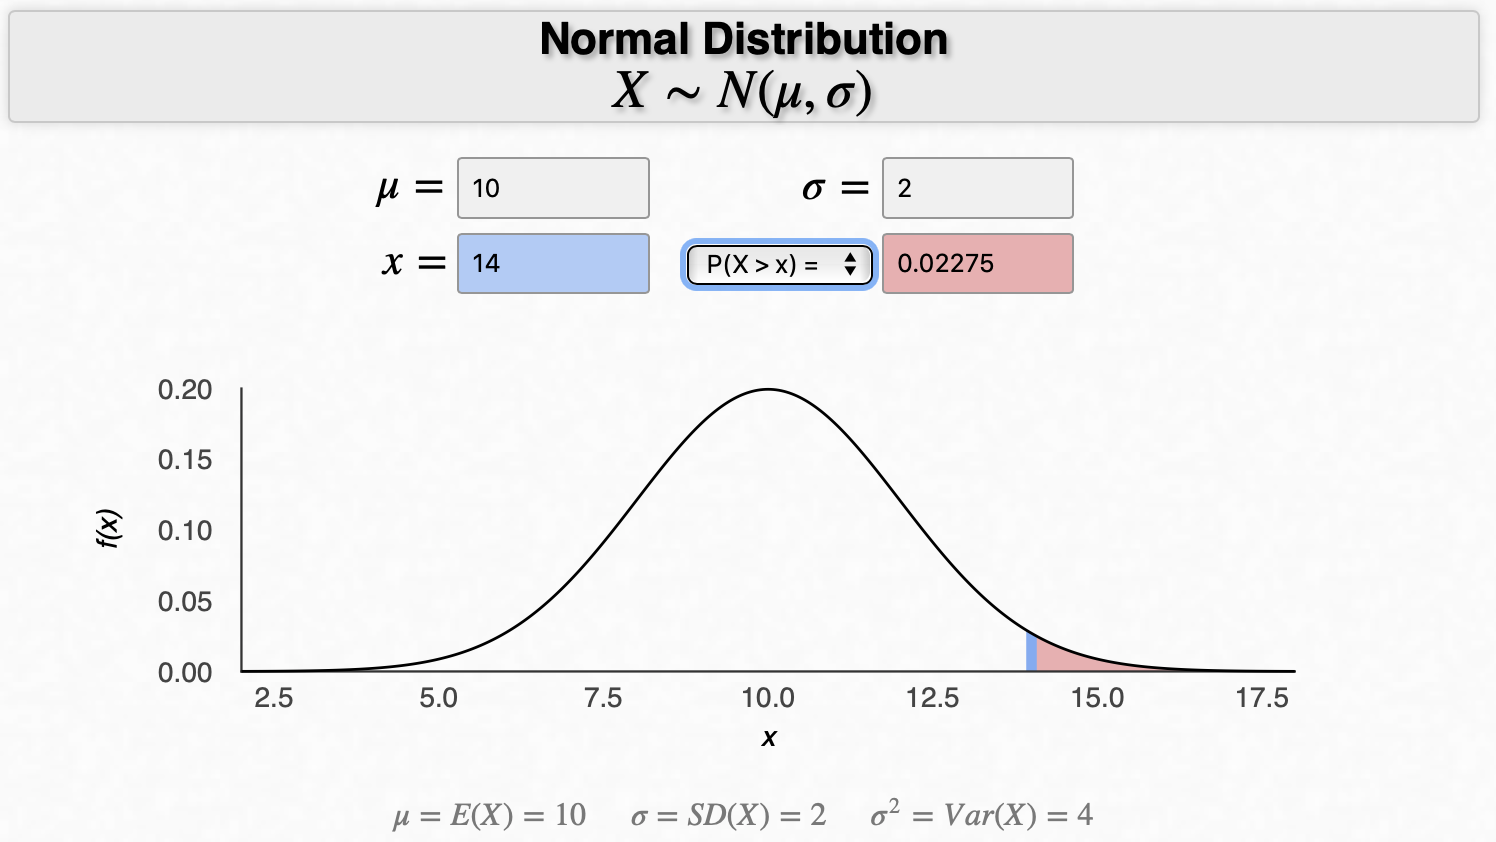
\includegraphics[width=20.78in]{img/3_3}

\hypertarget{pregunta-test-111}{%
\section{Pregunta test}\label{pregunta-test-111}}

Se realiza un estudio para saber si dos tratamientos de quimioterapia presentan diferencias en cuanto a la supervivencia de los pacientes. No se encontró diferencia estadísticamente significativa. ¿Cuál de las siguientes razones podrían ser causantes del resultado?

\begin{enumerate}
\def\labelenumi{\alph{enumi})}
\tightlist
\item
  Los tratamientos ofrecen tiempos de supervivencia muy diferentes.
\item
  El nivel de significación es demasiado alto.
\item
  Las muestras son demasiado numerosas.
\item
  Las muestras son demasiado pequeñas.
\item
  Nada de lo anterior.
\end{enumerate}

Respuesta correcta

\href{https://1fjmanzano.github.io/bioestadistica/contrastes-de-hipo\%CC\%81tesis.html}{Explicación}

\hypertarget{pregunta-test-112}{%
\section{Pregunta test}\label{pregunta-test-112}}

Se realiza un experimento donde nos basaremos en un contraste de hipótesis para tomar una decisión con un nivel de significación del 1\%. De las siguientes cuál no es un resultado posible de un contraste de hipótesis:

\begin{enumerate}
\def\labelenumi{\alph{enumi})}
\tightlist
\item
  El experimento no es concluyente.
\item
  El experimento permite obtener conclusiones.
\item
  Se rechaza la hipótesis nula.
\item
  Se rechaza la hipótesis alternativa.
\item
  Se acepta la hipótesis alternativa.
\end{enumerate}

Respuesta correcta

\href{https://1fjmanzano.github.io/bioestadistica/contrastes-de-hipo\%CC\%81tesis.html}{Explicación}

\hypertarget{pregunta-test-113}{%
\section{Pregunta test}\label{pregunta-test-113}}

El IMC se distribuye en una población de forma normal. El 95\% central de los individuos tiene un IMC comprendido entre 20 y 24. Entonces:

\begin{enumerate}
\def\labelenumi{\alph{enumi})}
\tightlist
\item
  La media es 22.
\item
  La desviación típica es 1.
\item
  La curtosis es cero.
\item
  Todas las anteriores son correctas.
\item
  Sólo dos de las anteriores son correctas.
\end{enumerate}

Respuesta correcta

\href{https://1fjmanzano.github.io/bioestadistica/distribuciones-de-probabilidad.html\#distribucio\%CC\%81n-normal}{Explicación}

\hypertarget{pregunta-test-114}{%
\section{Pregunta test}\label{pregunta-test-114}}

Elija la afirmación \textbf{falsa}:

\begin{enumerate}
\def\labelenumi{\alph{enumi})}
\tightlist
\item
  El nivel de significación es normalmente un valor pequeño.
\item
  La significación de un contraste es conocida tras analizar los datos.
\item
  El nivel de significación de un contraste debe ser fijado antes de analizar los datos.
\item
  Un contraste debe ser declarado significativo antes de recoger los datos.
\item
  Un contraste es declarado significativo si se obtiene una muestra que discrepa mucho de la hipótesis nula.
\end{enumerate}

Respuesta correcta

\href{https://1fjmanzano.github.io/bioestadistica/contrastes-de-hipo\%CC\%81tesis.html}{Explicación}

\hypertarget{problema-14}{%
\section{Problema}\label{problema-14}}

El tiempo que los empleados de una oficina tardan en completar una tarea específica sigue una distribución normal con una media de 45 minutos y una desviación típica de 5 minutos. ¿Cuál es el tiempo que separa aproximadamente al 16\% más rápido de los empleados del resto?

\hypertarget{explicaciuxf3n}{%
\subsection{Explicación}\label{explicaciuxf3n}}

Este es un problema de distribución normal inversa \href{https://youtu.be/BqGHUqC4cdQ}{Ver vídeo}.

Si utilizamos la aplicación \href{https://homepage.divms.uiowa.edu/~mbognar/applets/normal.html}{Probability Distributios: Normal Distribution} no tenemos más que introducir los valores \(\mu = 45\), \(\sigma = 5\) y \(P(X > x)= 0.16\) para obtener un valor de \(x = 49.97229 \approx 50\).

Entonces, \textbf{l tiempo que separa aproximadamente al 16\% más rápido de los empleados del resto es de 50 minutos}.

\hypertarget{pregunta-test-115}{%
\section{Pregunta test}\label{pregunta-test-115}}

Los ingresos de un grupo de personas siguen una distribución normal con una media de 50,000 € y una desviación típica de 10,000 €. ¿Cuál es el rango aproximado de ingresos que abarca al 95\% de las personas en este grupo?

a Entre 30,000€ y 70,000€
b Entre 20,000€ y 80,000€
c Entre 40,000€ y 60,000€
d Entre 10,000€ y 90,000€
e Entre 50,000€ y 100,000€

Respuesta correcta

\href{https://youtu.be/TjZvZVxItLc}{Explicación}

\hypertarget{pregunta-test-116}{%
\section{Pregunta test}\label{pregunta-test-116}}

La cantidad de tiempo que los estudiantes tardan en completar un examen sigue una distribución normal con una media de 120 minutos y una desviación típica de 20 minutos. ¿Qué porcentaje de estudiantes termina el examen en menos de 100 minutos?

\begin{enumerate}
\def\labelenumi{\alph{enumi})}
\tightlist
\item
  2.5\%
\item
  5\%
\item
  16\%
\item
  34\%
\item
  50\%
\end{enumerate}

Respuesta correcta

\href{https://homepage.divms.uiowa.edu/~mbognar/applets/normal.html}{Explicación}

\hypertarget{pregunta-test-117}{%
\section{Pregunta test}\label{pregunta-test-117}}

Solamente una de las siguientes frases podría alguna vez encontrarse como conclusión de un estudio científico. ¿Cuál es?

\begin{enumerate}
\def\labelenumi{\alph{enumi})}
\tightlist
\item
  El tratamiento produjo un efecto significativamente mayor que el placebo (p=0.75)
\item
  El tratamiento produjo un efecto significativamente menor que el placebo (p=0.25)
\item
  El tratamiento no produjo un resultado diferente al placebo (p\textless0.001)
\item
  El tratamiento produjo un efecto significativamente menor que el placebo (p=0.99)
\item
  Se apreciaban diferencias significativas entre el placebo y el tratamiento (p\textless0.001)
\end{enumerate}

Respuesta correcta

\href{https://1fjmanzano.github.io/bioestadistica/contrastes-de-hipo\%CC\%81tesis.html\#contrastes-bilaterales-y-unilaterales}{Explicación}

\hypertarget{pregunta-test-118}{%
\section{Pregunta test}\label{pregunta-test-118}}

En un estudio que investiga la eficacia de una nueva terapia de rehabilitación para pacientes que han sufrido un accidente cerebrovascular, solo una de las siguientes afirmaciones cumple con los criterios de significación estadística. ¿Cuál es?

\begin{enumerate}
\def\labelenumi{\alph{enumi})}
\tightlist
\item
  La nueva terapia no mostró diferencias significativas en la recuperación en comparación con la terapia estándar (p=0.90)
\item
  La nueva terapia fue significativamente menos efectiva que la terapia estándar (p=0.14)
\item
  La nueva terapia fue significativamente más efectiva que la terapia estándar (p\textless0.001)
\item
  La nueva terapia fue igual de efectiva que la terapia estándar (p=0.51)
\item
  La terapia estándar fue significativamente más efectiva que la nueva terapia (p=0.68)
\end{enumerate}

Respuesta correcta

\href{https://1fjmanzano.github.io/bioestadistica/contrastes-de-hipo\%CC\%81tesis.html\#contrastes-bilaterales-y-unilaterales}{Explicación}

\hypertarget{pregunta-test-119}{%
\section{Pregunta test}\label{pregunta-test-119}}

La duración de las llamadas en un centro de atención al cliente sigue una distribución normal con una media de 8 minutos y una desviación típica de 2 minutos. ¿Cuál es el tiempo que separa aproximadamente al 2.5\% de las llamadas más cortas del resto?

\begin{enumerate}
\def\labelenumi{\alph{enumi})}
\tightlist
\item
  2 minutos
\item
  4 minutos
\item
  6 minutos
\item
  10 minutos
\item
  12 minutos
\end{enumerate}

Respuesta correcta

\href{https://homepage.divms.uiowa.edu/~mbognar/applets/normal.html}{Explicación}

\hypertarget{pregunta-test-120}{%
\section{Pregunta test}\label{pregunta-test-120}}

En un estudio que evalúa la efectividad de la terapia cognitivo-conductual (TCC) en comparación con la terapia de apoyo en el tratamiento de la ansiedad, solo una de las siguientes afirmaciones es correcta según los criterios de significación estadística. ¿Cuál es?

\begin{enumerate}
\def\labelenumi{\alph{enumi})}
\tightlist
\item
  La TCC no mostró diferencias significativas en la reducción de la ansiedad en comparación con la terapia de apoyo (p=0.15)
\item
  La TCC fue significativamente más efectiva que la terapia de apoyo en la reducción de la ansiedad (p\textless0.001)
\item
  La terapia de apoyo fue significativamente más efectiva que la TCC en la reducción de la ansiedad (p=0.91)
\item
  Ambas terapias fueron igualmente efectivas en la reducción de la ansiedad (p=0.06)
\item
  La TCC fue significativamente menos efectiva que la terapia de apoyo en la reducción de la ansiedad (p=0.56)
\end{enumerate}

Respuesta correcta

\hypertarget{pregunta-test-121}{%
\section{Pregunta test}\label{pregunta-test-121}}

En una población de estudiantes, las calificaciones en matemáticas tienen una media de 75 y una desviación típica de 10, mientras que las calificaciones en ciencias tienen una media de 80 y una desviación típica de 5. Un estudiante obtiene una calificación de 90 en matemáticas y 85 en ciencias. ¿Cuál de las siguientes afirmaciones es correcta?

\begin{enumerate}
\def\labelenumi{\alph{enumi})}
\tightlist
\item
  La calificación de matemáticas es más extrema que la de ciencias.
\item
  La calificación de ciencias es más extrema que la de matemáticas.
\item
  Las calificaciones de matemáticas y ciencias son igualmente extremas.
\item
  La calificación de matemáticas es menos extrema que la de ciencias.
\item
  No se pueden comparar ambas calificaciones.
\end{enumerate}

Respuesta correcta

\href{https://homepage.divms.uiowa.edu/~mbognar/applets/normal.html}{Explicación}

\hypertarget{regresiuxf3n-y-correlaciuxf3n.}{%
\chapter{Regresión y correlación.}\label{regresiuxf3n-y-correlaciuxf3n.}}

En este capítulo se resolverán problemas relativos a:

\begin{itemize}
\tightlist
\item
  Introducción a la regresión y correlación
\item
  Estudio de la representatividad de la recta de regresión
\item
  Otros modelos de regresión
\item
  Correlación
\end{itemize}

\hypertarget{pregunta-test-122}{%
\section{Pregunta test}\label{pregunta-test-122}}

Si al calcular el coeficiente de correlación de dos variables X e Y, se tiene r=-0.20 ocurre que:

\begin{enumerate}
\def\labelenumi{\alph{enumi})}
\tightlist
\item
  La pendiente de la recta de regresión es pequeña.
\item
  La pendiente de la recta de regresión es grande.
\item
  X e Y están poco relacionadas, aunque cuando X decrece, Y tiene tendencia a crecer.
\item
  El modelo lineal de regresión explica el 20\% de la varianza de una variable cualquiera en función de la otra.
\item
  El modelo lineal de regresión explica el 80\% de la varianza de una variable cualquiera en función de la otra.
\end{enumerate}

Respuesta correcta

\href{https://1fjmanzano.github.io/bioestadistica/relaci\%C3\%B3n-entre-variables-nume\%CC\%81ricas.html}{Explicación}

\hypertarget{pregunta-test-123}{%
\section{Pregunta test}\label{pregunta-test-123}}

La recta de regresión de Y sobre X se muestra como un buen modelo para explicar la relación entre dos variables numéricas. Entonces:

\begin{enumerate}
\def\labelenumi{\alph{enumi})}
\tightlist
\item
  Y se puede calcular exactamente como una función matemática de X.
\item
  Y es independiente de X.
\item
  La covarianza de X e Y no es nula.
\item
  La media de X coincide con la media de Y.
\item
  Sólo dos de las afirmaciones anteriores son correctas.
\end{enumerate}

Respuesta correcta

\href{https://1fjmanzano.github.io/bioestadistica/relaci\%C3\%B3n-entre-variables-nume\%CC\%81ricas.html\#covarianza}{Explicación}

\hypertarget{pregunta-test-124}{%
\section{Pregunta test}\label{pregunta-test-124}}

En una población se obtiene con una bondad de ajuste de 0,9 que la relación entre nivel de glucemia (Y) y nivel de colesterol (X) es de \(Y=20 + \dfrac{X}{4}\). Entonces:

\begin{enumerate}
\def\labelenumi{\alph{enumi})}
\tightlist
\item
  Todos los individuos con un valor de colesterol 100, presentan glucemia 45.
\item
  Existe tendencia a que a mayor nivel de glucemia, mayor nivel de colesterol.
\item
  Hay mas individuos con colesterol alto que con glucemia baja.
\item
  Las observaciones se muestran como una nube de puntos creciente.
\item
  Sólo dos de las afirmaciones anteriores son correctas.
\end{enumerate}

Respuesta correcta

\textbf{Explicación}

Tenemos que \(r = 0.9\) lo que indica una correlacion lineal positiva y fuerte entre las 2 variables.

Además, tenemos la ecuación de la recta de regresión de \(Y\) (nivel de glucemia) sobre \(X\) (nivel de colesterol), \(Y=20 + \dfrac{X}{4}\)

Veamos cada apartado:

\textbf{a)} Efectivamente, para un valor de colesterol 100, como \(Y=20 + \dfrac{100}{4}= 20 + 25 = 45\), se estima que el valor de glucemia es de 45. Pero eso no implica que \emph{todos los individuos} con un valor de colesterol 100, presentan glucemia 45.

\textbf{b)} Al haber correlación lineal positiva y fuerte (\(r^2=0.9 \Rightarrow r \approx 0.95\)), se cumple que existe tendencia a que a mayor nivel de glucemia, mayor nivel de colesterol.

\textbf{c)} Con los datos del problema, no podemos saber si hay mas individuos con colesterol alto que con glucemia baja.

\textbf{d)} Como la nube de puntos se ajusta bastante bien a la recta de regresión cuya gráfica (obtenida con \href{https://www.desmos.com/calculator?lang=es}{Desmos}) es:

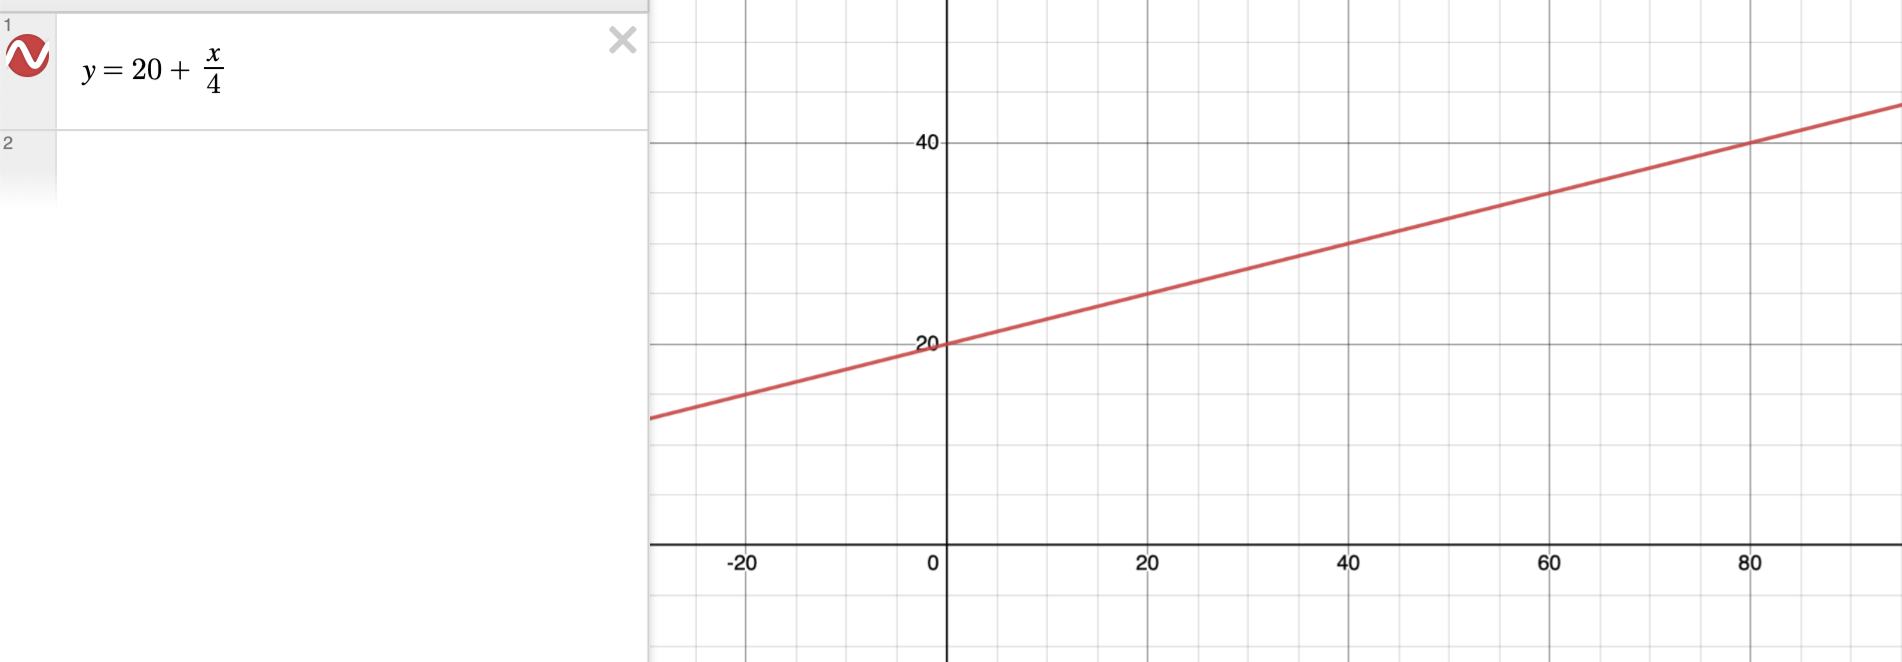
\includegraphics[width=26.42in]{img/4_1}

se cumple que las observaciones se muestran como una nube de puntos creciente.

\hypertarget{pregunta-test-125}{%
\section{Pregunta test}\label{pregunta-test-125}}

Dos variables numéricas son incorreladas. Entonces:

\begin{enumerate}
\def\labelenumi{\alph{enumi})}
\tightlist
\item
  \(r = 0\)
\item
  El modelo lineal de regresión sólo propone un valor como predicción de \(Y\).
\item
  La nube de puntos no presenta aspecto creciente.
\item
  La varianza residual en el modelo de regresión de Y sobre X es igual a la varianza de Y.
\item
  Todo lo anterior es cierto.
\end{enumerate}

Respuesta correcta

\textbf{Explicación}

\textbf{a)} Si no existe correlación entre las variables (incorreladas), \(r=0\). Al mínimo de correlación que haya, \(r \neq 0\), tanto positiva como negativa.

\textbf{b)} Siempre se cumple que el modelo lineal de regresión sólo propone un valor como predicción de \(Y\). Al obtener la ecuación de la recta de regresión (modelo), para un valor de \(X\) únicamente tenemos un valor de \(Y\).

\textbf{c)} Al no haber correlación, la nube de puntos no presenta tendencia alguna por lo que la nube de puntos no presenta aspecto creciente (ni decreciente).

\textbf{d)} Recordamos que, modelo de regresión de Y sobre X, los residuos son las direfencias (en vertical) de los puntos a la recta de regresión, es decir las medidas del los segmentos de la imagen:

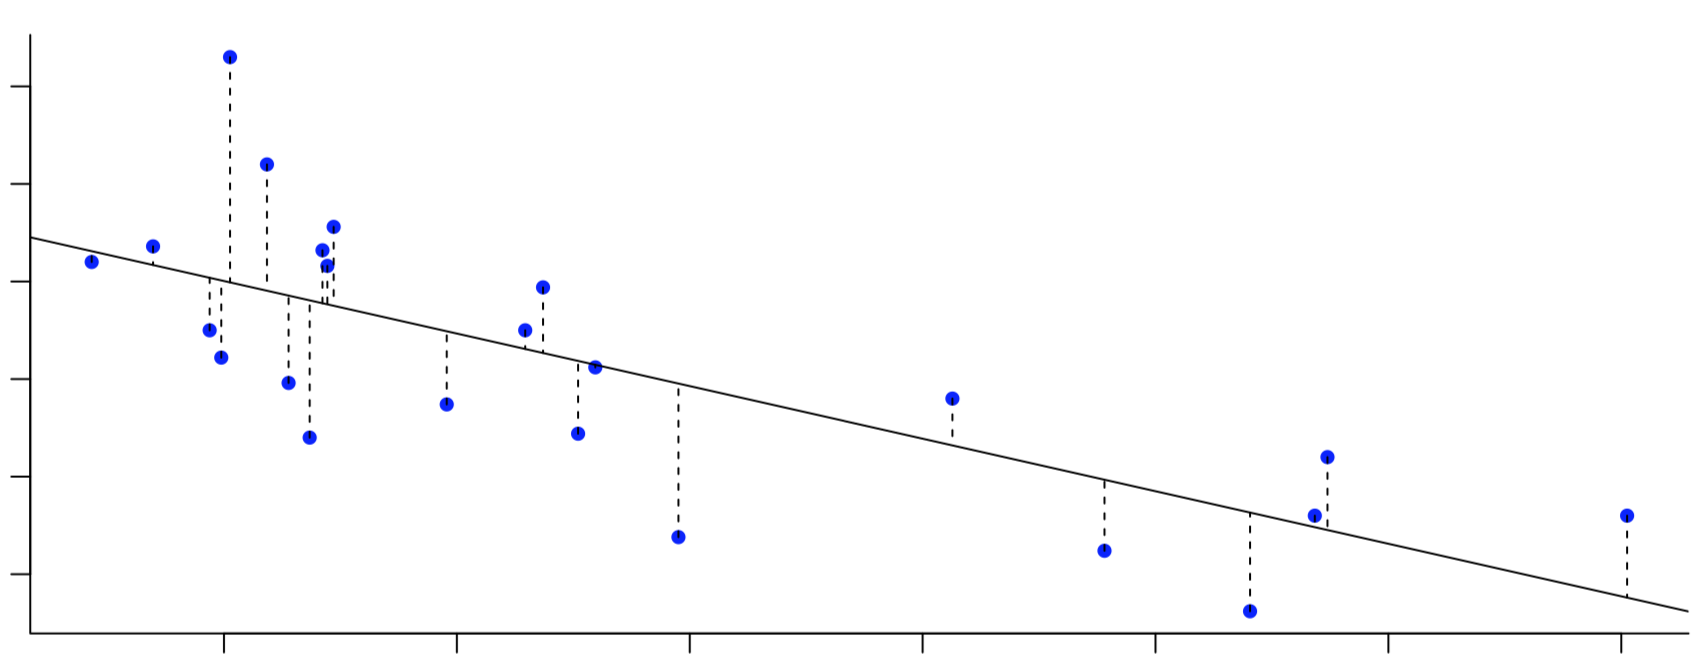
\includegraphics[width=23.72in]{img/4_2}

Así, la varianza residual en el modelo de regresión de Y sobre X es la media de los cuadrados de esos valores (residuos). Si la recta es oblicua, esos residuos dependen de esa inclinación, esto es, dependen de \(X\) e \(Y\).

En nuestro caso, las variables son incorreladas por lo que la recta de regresión del modelo de regresión de Y sobre X es horizontal:

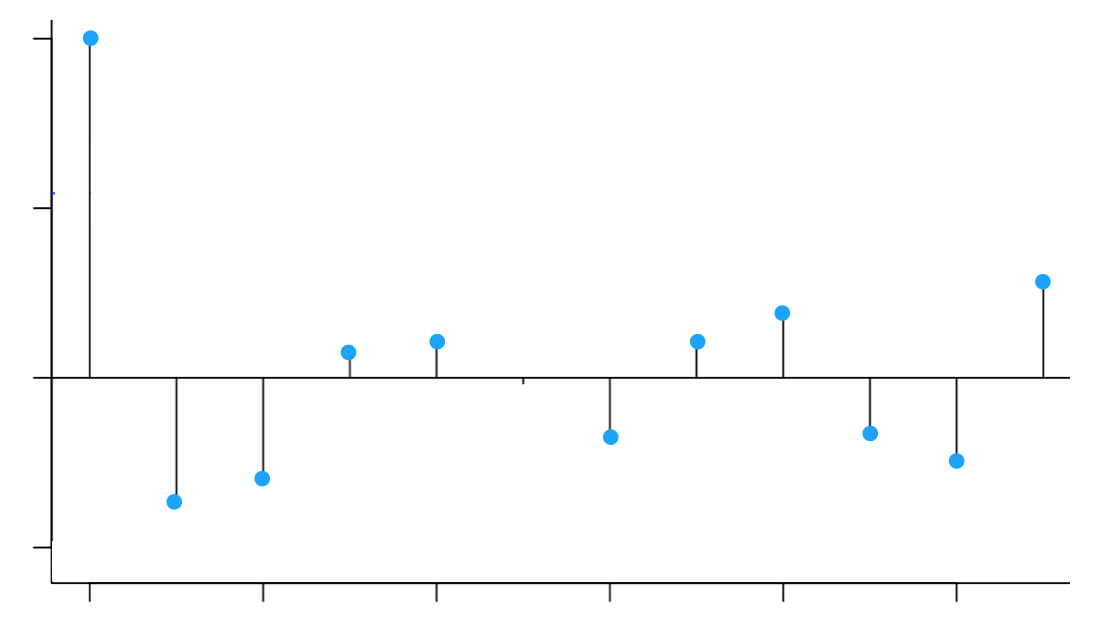
\includegraphics[width=15.42in]{img/4_3}

De este modo, los residuos dependen únicamente de \(Y\). Al pasar la recta de regresión por el punto \((\overline{x}, \overline{y})\), la media de los cuadrados de los residuos coincide con la varianza de \(Y\) por lo que, cuando las variables son incorreladas, la varianza residual en el modelo de regresión de Y sobre X es igual a la varianza de Y.

\hypertarget{pregunta-test-126}{%
\section{Pregunta test}\label{pregunta-test-126}}

De las siguientes parejas de variables, en cuáles crees que puede ser útil un análisis de regresión lineal:

\begin{enumerate}
\def\labelenumi{\alph{enumi})}
\tightlist
\item
  La presión sanguínea y el grupo sanguíneo.
\item
  El nivel de colesterol y la concentración de bilirrubina.
\item
  El grupos sanguíneo y el factor Rh.
\item
  El género y la edad.
\item
  Poseer ideología racista y el factor RH.
\end{enumerate}

Respuesta correcta

\href{https://smiba.org.ar/curso_medico_especialista/lecturas_2021/e\%29.\%204\%20Correlación\%20y\%20regresión.pdf}{Explicación}

\hypertarget{pregunta-test-127}{%
\section{Pregunta test}\label{pregunta-test-127}}

Si el coeficiente de correlación lineal de Pearson entre dos variables es \(-0,8\) podemos decir:

\begin{enumerate}
\def\labelenumi{\alph{enumi})}
\tightlist
\item
  La covarianza es negativa.
\item
  La relación entre las variables es directa.
\item
  Hay poca relación lineal entre las variables.
\item
  Hay un error de cálculo.
\item
  El 80\% de las predicciones son correctas.
\end{enumerate}

Respuesta correcta

\href{https://1fjmanzano.github.io/bioestadistica/relaci\%C3\%B3n-entre-variables-nume\%CC\%81ricas.html\#coeficiente-de-correlacio\%CC\%81n}{Explicación}

\hypertarget{pregunta-test-128}{%
\section{Pregunta test}\label{pregunta-test-128}}

En un estudio de regresión lineal, donde el peso se estudie conjuntamente con otras variables, en qué casos lo usarías como variable dependiente:

\begin{enumerate}
\def\labelenumi{\alph{enumi})}
\tightlist
\item
  Al estudiarlo con la altura.
\item
  Al estudiarlo con el nivel del colesterol.
\item
  Al estudiarlo con la presión sanguínea.
\item
  Al estudiarlo con el grupo sanguíneo.
\item
  Nada de lo anterior.
\end{enumerate}

Respuesta correcta

\href{https://www.cdc.gov/healthyweight/spanish/assessing/bmi/adult_bmi/index.html}{Explicación}

\hypertarget{pregunta-test-129}{%
\section{Pregunta test}\label{pregunta-test-129}}

En una población formada por unidades familiares, la altura media del padre en la familia se comporta como una distribución normal de media 170 cm con desviación típica 5 cm. La altura del primer hijo varón es otra variable con distribución similar. Con estos datos podemos afirmar:

\begin{enumerate}
\def\labelenumi{\alph{enumi})}
\tightlist
\item
  No hay relación entre ambas variables.
\item
  Hay relación inversa entre las variables.
\item
  No debemos intentar predecir la altura del hijo de un padre que mide 140 cm.
\item
  Hay relación directa entre las variables.
\item
  Nada de lo anterior.
\end{enumerate}

Respuesta correcta

\href{https://www.feedingthemachine.ai/regresion-lineal-y-los-outliers/}{Explicación}

\hypertarget{pregunta-test-130}{%
\section{Pregunta test}\label{pregunta-test-130}}

Se observa que al aumentar el consumo de estanol, disminuye el nivel de colesterol en sangre. Se utiliza un modelo de regresión lineal donde el nivel de colesterol es la variable independiente y el consumo de estanol es la dependiente. Se calcula una bondad de ajuste para el modelo del 25\%. Entonces:

\begin{enumerate}
\def\labelenumi{\alph{enumi})}
\tightlist
\item
  El 25\% de las predicciones del modelo son correctas.
\item
  \(r= 0.5\)
\item
  \(r= 0.25\)
\item
  \(r= -0.25\)
\item
  \(r= -0.5\)
\end{enumerate}

Respuesta correcta

\href{https://blog.minitab.com/es/analisis-de-regresion-como-puedo-interpretar-el-r-cuadrado-y-evaluar-la-bondad-de-ajuste}{Explicación}

\hypertarget{pregunta-test-131}{%
\section{Pregunta test}\label{pregunta-test-131}}

Si el coeficiente de correlación lineal de Pearson entre dos variables es -0,1 podemos decir:

\begin{enumerate}
\def\labelenumi{\alph{enumi})}
\tightlist
\item
  La covarianza es pequeña.
\item
  Hay fuerte relación inversa entre las variables.
\item
  Hay poca relación lineal entre las variables.
\item
  Hay un error de cálculo.
\item
  El 10\% de las predicciones son correctas.
\end{enumerate}

Respuesta correcta

\href{https://1fjmanzano.github.io/bioestadistica/relaci\%C3\%B3n-entre-variables-nume\%CC\%81ricas.html\#coeficiente-de-correlacio\%CC\%81n}{Explicación}

\hypertarget{pregunta-test-132}{%
\section{Pregunta test}\label{pregunta-test-132}}

Se estudia la asociación lineal entre dos variables numéricas. El coeficiente de determinación vale \(0,95\).

\begin{enumerate}
\def\labelenumi{\alph{enumi})}
\tightlist
\item
  Hay poca asociación.
\item
  Hay asociación directa.
\item
  Hay asociación inversa.
\item
  Hay una buena asociación
\item
  Nada de lo anterior.
\end{enumerate}

Respuesta correcta

\href{https://es.wikipedia.org/wiki/Coeficiente_de_determinación}{Explicacion}

\hypertarget{pregunta-test-133}{%
\section{Pregunta test}\label{pregunta-test-133}}

Se observa que al disminuir el consumo de comida rápida, disminuye el nivel de colesterol en sangre. Se usa un modelo de regresión entre ambas que ofrece una bondad de ajuste del 36\%. Entonces:

\begin{enumerate}
\def\labelenumi{\alph{enumi})}
\tightlist
\item
  El 36\% de las predicciones del modelo son correctas.
\item
  \(r= +0.60\)
\item
  \(r= +0.36\)
\item
  \(r= -0.60\)
\item
  \(r= -0.36\)
\end{enumerate}

Respuesta correcta

\href{https://es.wikipedia.org/wiki/Coeficiente_de_determinación}{Explicacion}

\hypertarget{pregunta-test-134}{%
\section{Pregunta test}\label{pregunta-test-134}}

Un modelo de regresión lineal para calcular la glucemia (sangre) a partir de la de la orina (glucosuria) es``glucemia = 20 + 0.5 glucosuria''. Si dos personas se diferencian en 10 unidades de glucosuria, cual es la mejor estimación que puede hacer para la diferencia en glucemia:

\begin{enumerate}
\def\labelenumi{\alph{enumi})}
\tightlist
\item
  5
\item
  10
\item
  15
\item
  20
\item
  25
\end{enumerate}

Respuesta correcta

\textbf{Explicacion}

El modelo establece que ``glucemia = 20 + 0.5 glucosuria''. Así, la pendiente (o inclinación) de la recta de regresión es \(0.5 = \frac{1}{2}\)

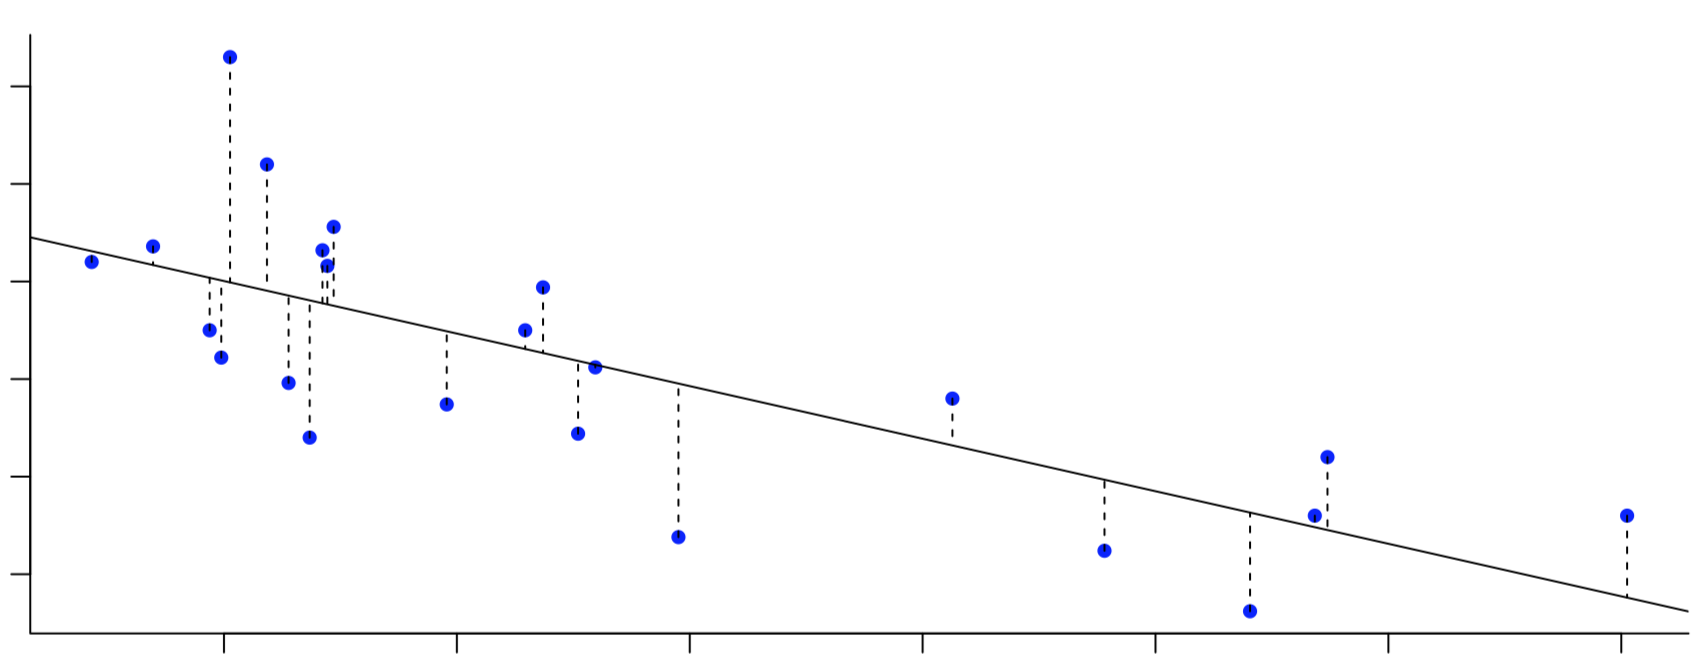
\includegraphics[width=23.72in]{img/4_2}

De este modo, si dos personas se diferencian en 10 unidades de glucosuria (en horizontal), la variación en glucemia (en vertical según el modelo) será la mitad, es decir, 5.

\hypertarget{pregunta-test-135}{%
\section{Pregunta test}\label{pregunta-test-135}}

Qué afirmación sobre la covarianza es falsa:

\begin{enumerate}
\def\labelenumi{\alph{enumi})}
\tightlist
\item
  La covarianza es una medida de la variabilidad conjunta de dos variables numéricas.
\item
  Si la covarianza es positiva implica una relación creciente entre las variables.
\item
  A partir de ella se obtiene el coeficiente de correlació lineal de Pearson.
\item
  Posee dimensiones.
\item
  Si es 0 podemos afirmar que no existe relación posible entre las variables.
\end{enumerate}

Respuesta correcta

\href{https://1fjmanzano.github.io/bioestadistica/relaci\%C3\%B3n-entre-variables-nume\%CC\%81ricas.html\#covarianza}{Explicacion}

\hypertarget{pregunta-test-136}{%
\section{Pregunta test}\label{pregunta-test-136}}

La pendiente de una recta de una función de regresión lineal es \(Y = b_0 + b_1 \cdot X\)

\begin{enumerate}
\def\labelenumi{\alph{enumi})}
\tightlist
\item
  Representa el incremento de \(Y\) por cada unidad de incremento de \(X\).
\item
  Tiene el mismo signo que la covarianza.
\item
  Es el valor de la variable \(Y\) cuando \(X=0\).
\item
  Todas las anteriores son correctas.
\item
  Sólo la a) y la b) son correctas.
\end{enumerate}

Respuesta correcta

\href{https://1fjmanzano.github.io/bioestadistica/relaci\%C3\%B3n-entre-variables-nume\%CC\%81ricas.html\#regresio\%CC\%81n-lineal}{Explicacion}

\hypertarget{pregunta-test-137}{%
\section{Pregunta test}\label{pregunta-test-137}}

De los siguiente estudios de relación entre variables, en cuál crees que no sería oportuno usar la técnica de regresión lineal.

\begin{enumerate}
\def\labelenumi{\alph{enumi})}
\tightlist
\item
  La presión sanguínea y la acidez (ph).
\item
  El número de glóbulos rojos y el grupo sanguíneo
\item
  La altura y las horas de sueño.
\item
  La edad y el conteo de plaquetas.
\item
  El nivel de colesterol y la concentración de bilirrubina.
\end{enumerate}

Respuesta correcta

\href{https://es.cochrane.org/es/divulgacion/pensamiento-critico/correlacion-no-implica-causalidad}{Explicacion}

\hypertarget{pregunta-test-138}{%
\section{Pregunta test}\label{pregunta-test-138}}

Después de estudiar la relación existente entre la flexión y la extensión de cuello de los alumnos de la USAL, obtenemos que el valor de la covarianza es \(-0,57\). ¿El valor de r saldrá positivo o negativo?

\begin{enumerate}
\def\labelenumi{\alph{enumi})}
\tightlist
\item
  Saldrá positivo porque la relación es inversa.
\item
  Saldrá negativo también porque el signo de la covarianza y del coeficiente de correlación lineal de Pearson siempre coinciden.
\item
  No podemos saber el signo de r sabiendo la covarianza porque no están relacionados.
\item
  Todas las anteriores son falsas.
\item
  Necesitamos conocer \(R^2\) para saber el signo de r
\end{enumerate}

Respuesta correcta

\href{https://1fjmanzano.github.io/bioestadistica/relaci\%C3\%B3n-entre-variables-nume\%CC\%81ricas.html\#covarianza}{Explicacion}

\hypertarget{pregunta-test-139}{%
\section{Pregunta test}\label{pregunta-test-139}}

Si el coeficiente de correlación lineal de Pearson entre dos variables es \(-0,9\) podemos decir que:

\begin{enumerate}
\def\labelenumi{\alph{enumi})}
\tightlist
\item
  La covarianza será positiva.
\item
  La relación lineal es buena.
\item
  Al ser inferior a 1, la relación lineal es pequeña.
\item
  Tenemos una relación lineal inversa, pero no buena.
\item
  Sólo dos son correctas.
\end{enumerate}

Respuesta correcta

\href{https://1fjmanzano.github.io/bioestadistica/relaci\%C3\%B3n-entre-variables-nume\%CC\%81ricas.html\#coeficiente-de-correlacio\%CC\%81n}{Explicacion}

\hypertarget{pregunta-test-140}{%
\section{Pregunta test}\label{pregunta-test-140}}

Cual de las siguientes propiedades de r son correctas:

\begin{enumerate}
\def\labelenumi{\alph{enumi})}
\tightlist
\item
  Es adimensional
\item
  Cuanto más cerca esté r de de +1 o -1 mejor será el grado de relación lineal
\item
  Las variables son incorreladas cuando r=0
\item
  Todas las anteriores son correctas
\item
  Son todas incorrectas
\end{enumerate}

Respuesta correcta

\href{https://1fjmanzano.github.io/bioestadistica/relaci\%C3\%B3n-entre-variables-nume\%CC\%81ricas.html\#coeficiente-de-correlacio\%CC\%81n}{Explicacion}

\hypertarget{pregunta-test-141}{%
\section{Pregunta test}\label{pregunta-test-141}}

Se dice que la relación entre dos variables es directa cuando:

\begin{enumerate}
\def\labelenumi{\alph{enumi})}
\tightlist
\item
  La covarianza es igual a cero
\item
  La covarianza es negativa
\item
  La covarianza es mayor que cero
\item
  El coeficiente de correlación lineal es positivo
\item
  Las respuestas c) y d) son correctas
\end{enumerate}

Respuesta correcta

\href{https://1fjmanzano.github.io/bioestadistica/relaci\%C3\%B3n-entre-variables-nume\%CC\%81ricas.html\#coeficiente-de-correlacio\%CC\%81n}{Explicacion}

\hypertarget{pregunta-test-142}{%
\section{Pregunta test}\label{pregunta-test-142}}

Sabiendo que \(r=+0.7\) elija la afirmación falsa.

\begin{enumerate}
\def\labelenumi{\alph{enumi})}
\tightlist
\item
  La covarianza es positiva
\item
  Hay cierta relación lineal entre las variables
\item
  La bondad de ajuste es 0.14
\item
  La nube de puntos es creciente
\item
  Existe una relación directa
\end{enumerate}

Respuesta correcta

\href{https://blog.minitab.com/es/analisis-de-regresion-como-puedo-interpretar-el-r-cuadrado-y-evaluar-la-bondad-de-ajuste}{Explicacion}

\hypertarget{pregunta-test-143}{%
\section{Pregunta test}\label{pregunta-test-143}}

En un estudio de regresión, ¿cuándo coincidirán los valores de la variable dependiente con los propuestos por el modelo lineal de regresión?

\begin{enumerate}
\def\labelenumi{\alph{enumi})}
\tightlist
\item
  Cuando r tenga un valor positivo
\item
  Cuando r sea igual a cero
\item
  Nunca, aunque el modelo sea perfecto
\item
  Cuando r valga 1 ó -1
\item
  Las opciones c) y d) son correctas
\end{enumerate}

Respuesta correcta

\href{https://1fjmanzano.github.io/bioestadistica/relaci\%C3\%B3n-entre-variables-nume\%CC\%81ricas.html\#coeficiente-de-correlacio\%CC\%81n}{Explicacion}

\hypertarget{pregunta-test-144}{%
\section{Pregunta test}\label{pregunta-test-144}}

Si el coeficiente de correlación lineal de Pearson entre dos variables es \(-0,82\), podemos afirmar que:

\begin{enumerate}
\def\labelenumi{\alph{enumi})}
\tightlist
\item
  la relación entre las dos variables es casi nula
\item
  la relación que hay entre las variables es muy buena y directa
\item
  la covarianza es positiva
\item
  la relación que hay entre las variables es muy buena e inversa
\item
  sólo dos de las afirmaciones anteriores son correctas
\end{enumerate}

Respuesta correcta

\href{https://1fjmanzano.github.io/bioestadistica/relaci\%C3\%B3n-entre-variables-nume\%CC\%81ricas.html\#coeficiente-de-correlacio\%CC\%81n}{Explicacion}

\hypertarget{pregunta-test-145}{%
\section{Pregunta test}\label{pregunta-test-145}}

¿Qué otro nombre reciben los diagramas de dispersión?

\begin{enumerate}
\def\labelenumi{\alph{enumi})}
\tightlist
\item
  Diagrama de regresión
\item
  Nube de puntos
\item
  Diagrama lineal
\item
  Diagrama de relación inversa
\item
  Diagrama simple
\end{enumerate}

Respuesta correcta

\href{https://1fjmanzano.github.io/bioestadistica/relaci\%C3\%B3n-entre-variables-nume\%CC\%81ricas.html\#diagramas-de-dispersio\%CC\%81n}{Explicacion}

\hypertarget{pregunta-test-146}{%
\section{Pregunta test}\label{pregunta-test-146}}

Un modelo de regresión lineal para calcular ``Fatty liver Index'' (\(FLI\)) a partir del consumo de \(aceite\) de oliva es ``\(FLI=70- 4 \cdot aceite\)''. Si dos personas se diferencian en 5 unidades de consumo de aceite, cual es la mejor estimación que puede hacer para la diferencia en \(FLI\):

\begin{enumerate}
\def\labelenumi{\alph{enumi})}
\tightlist
\item
  5
\item
  10
\item
  15
\item
  20
\item
  60
\end{enumerate}

Respuesta correcta

\href{https://1fjmanzano.github.io/bioestadistica/relaci\%C3\%B3n-entre-variables-nume\%CC\%81ricas.html\#regresio\%CC\%81n-lineal}{Explicacion}

\hypertarget{pregunta-test-147}{%
\section{Pregunta test}\label{pregunta-test-147}}

El porcentaje de variabilidad explicada por un modelo lineal de regresión es 3\%.

\begin{enumerate}
\def\labelenumi{\alph{enumi})}
\tightlist
\item
  El modelo lineal de regresión es insuficiente para explicar la variable dependiente.
\item
  Las variables son incorreladas.
\item
  El error cometido por el modelo lineal de regresión es pequeño, por tanto el ajuste lineal es bueno.
\item
  Hay una relación creciente entre las variables.
\item
  Todo lo anterior es falso.
\end{enumerate}

Respuesta correcta

\href{https://blog.minitab.com/es/analisis-de-regresion-como-puedo-interpretar-el-r-cuadrado-y-evaluar-la-bondad-de-ajuste}{Explicacion}

\hypertarget{pregunta-test-148}{%
\section{Pregunta test}\label{pregunta-test-148}}

Si en un experimento realizado sobre estudiantes voluntarios a los que se coloca en situación de estrés se observa que los cambios en ritmo cardíaco \(RC\) (latidos por minuto) se asocian a cambios en la frecuencia de la voz \(FV\) (Hz) con una bondad de ajuste del 15\% según el modelo \(FV = -5 + 3 \cdot RC\), marque la afirmación verdadera.

\begin{enumerate}
\def\labelenumi{\alph{enumi})}
\tightlist
\item
  La relación entre las variables es inversa.
\item
  Las variables no presentan ninguna relación.
\item
  La voz disminuye su frecuencia en 5Hz.
\item
  Por cada aumento de 1 latido por minuto cardíaco, se produce un aumento de 3 Hz en frecuencia de la voz,
\item
  Todo lo anterior es falso.
\end{enumerate}

Respuesta correcta

\href{https://1fjmanzano.github.io/bioestadistica/relaci\%C3\%B3n-entre-variables-nume\%CC\%81ricas.html\#regresio\%CC\%81n-lineal}{Explicacion}

\hypertarget{pregunta-test-149}{%
\section{Pregunta test}\label{pregunta-test-149}}

Un modelo de regresión lineal que relaciona el tiempo de estudio con el promedio obtenido en una prueba tiene una bondad de ajuste del 36\%. ¿Qué significa esto en términos de la relación entre el tiempo de estudio y el promedio obtenido?

\begin{enumerate}
\def\labelenumi{\alph{enumi})}
\tightlist
\item
  La relación es muy fuerte y positiva
\item
  La relación es muy débil y negativa
\item
  La relación es muy fuerte y negativa
\item
  La relación es muy débil y positiva
\item
  No se puede inferir la relación entre ambas variables a partir de la bondad de ajuste.
\end{enumerate}

Respuesta correcta

\href{https://blog.minitab.com/es/analisis-de-regresion-como-puedo-interpretar-el-r-cuadrado-y-evaluar-la-bondad-de-ajuste}{Explicacion}

\hypertarget{pregunta-test-150}{%
\section{Pregunta test}\label{pregunta-test-150}}

¿Cuál de las siguientes medidas estadísticas es la más adecuada para medir la relación entre el peso y la estatura de un grupo de personas?

\begin{enumerate}
\def\labelenumi{\alph{enumi})}
\tightlist
\item
  Rango intercuartílico
\item
  Desviación estándar
\item
  Coeficiente de variación
\item
  Coeficiente de correlación de Pearson
\item
  Coeficiente de asimetría
\end{enumerate}

Respuesta correcta

\href{https://1fjmanzano.github.io/bioestadistica/relaci\%C3\%B3n-entre-variables-nume\%CC\%81ricas.html\#coeficiente-de-correlacio\%CC\%81n}{Explicacion}

\hypertarget{tablas-de-contingencia.}{%
\chapter{Tablas de contingencia.}\label{tablas-de-contingencia.}}

En este capítulo se resolverán problemas relativos a:

\begin{itemize}
\tightlist
\item
  Contrastes de asociación y homogeneidad en tablas bifactoriales
\item
  Coeficientes de asociación
\end{itemize}

\hypertarget{problema-15}{%
\section{Problema}\label{problema-15}}

Un estudio transversal para conocer la prevalencia de osteoporosis y su relación con algunos factores de riesgo potenciales incluyó a 400 mujeres con edades entre 50 y 54 años. A cada una se le realizó una densitometría de columna y en cada caso se completó un cuestionario de antecedentes. Se pretende determinar si existe una asociación significativa entre la prevalencia de osteoporosis y antecedentes de dieta pobre en calcio. De las 80 pacientes que presentaban osteoporosis 58 presentaban antecedentes de dieta pobre en calcio, en tanto que entre las 320 que no tenían osteoporosis, el número de mujeres con este antecedente era de 62.

\textbf{a)} Construye la tabla de contingencia correspondiente y determina, para una nivel de significación del 1 \%, si existe una asociación significativa entre la prevalencia de osteoporosis y antecedentes de dieta pobre en calcio.

\textbf{b)} Calcula el estadístico Chi-cuadrado corregido (corrección de Yates) y determina en base a ese estadístico si, para un nivel de significación del 5 \%, existe una asociación significativa entre la prevalencia de osteoporosis y antecedentes de dieta pobre en calcio.

\textbf{c)} Calcula el riesgo relativo.

\hypertarget{soluciuxf3n-11}{%
\subsection{Solución}\label{soluciuxf3n-11}}

\textbf{a)} Incluimos los datos en una tabla de contingencia y la completamos:

\begin{longtable}[]{@{}cccc@{}}
\toprule
& Osteoporosis & No osteoporosis &\tabularnewline
\midrule
\endhead
Dieta pobre en calcio & 58 & 62 & 120\tabularnewline
Dieta rica en calcio & 22 & 258 & 280\tabularnewline
& 80 & 320 & 400\tabularnewline
\bottomrule
\end{longtable}

Establecemos la hipótesis nula y la alternativa:

\begin{itemize}
\tightlist
\item
  \(H_0:\) No hay asociación entre las variables (son independientes)
\item
  \(H_1:\) Sí hay asociación entre las variables
\end{itemize}

Ahora, necesitamos calcular el valor del estadístico chi-cuadrado y el valor p asociado para aceptar o rechazar la hipótesis nula. Para ello, podemos utilizar Excel© y seguir las instrucciones de \href{https://1fjmanzano.github.io/bioestadistica/me\%CC\%81todos-de-inferencia-estadi\%CC\%81stica.html\#prueba-chi2-pr\%C3\%A1ctica}{esta práctica del Curso de Bioestadística}

En este caso, vamos a utilizar la calculadora online \href{https://www.socscistatistics.com/tests/chisquare/default2.aspx}{Chi-Square Calculator} que nos da los siguientes resultados:

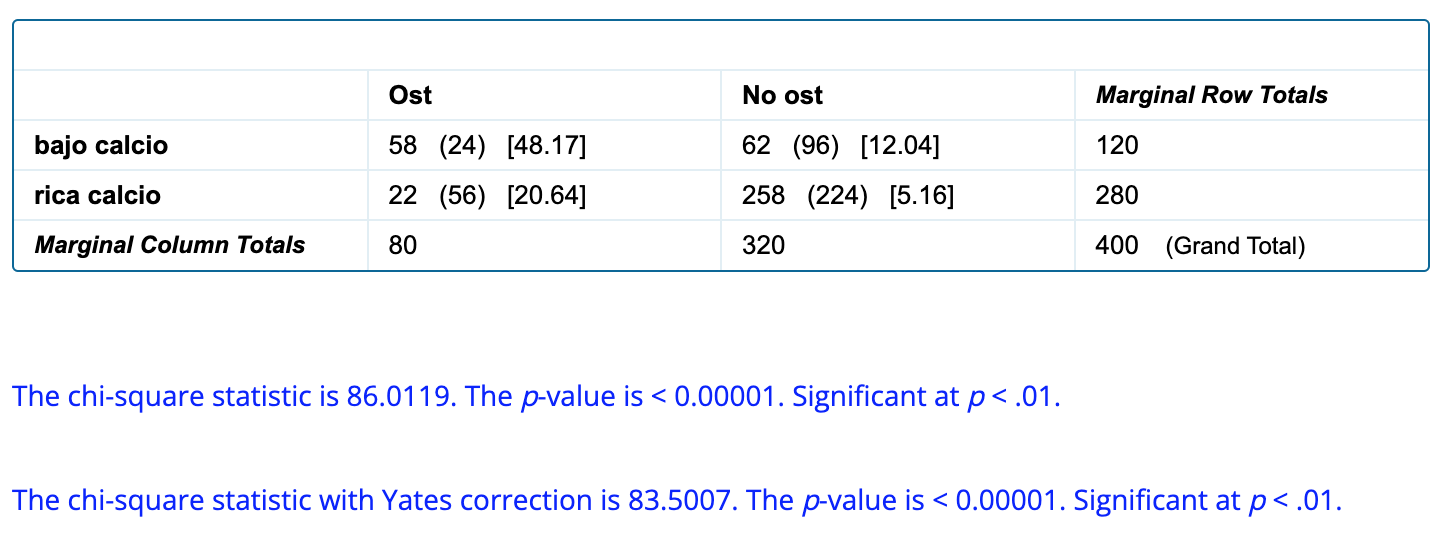
\includegraphics[width=20.11in]{img/5_1}

Así. el valor del estadístico Chi-cuadrado es 86.01 con un valor p asociado \textless{} 0.00001. Se rechaza la hipótesis de independencia al 1\%: hay relación significativa entre padecer osteoporosis y tener antecedentes de dieta pobre en calcio.

\textbf{b)} Nos piden ahora el valor del estadístico Chi-cuadrado corregido (corrección de Yates) para un nivel de significación del 5\% (0.05). Obtenemos:

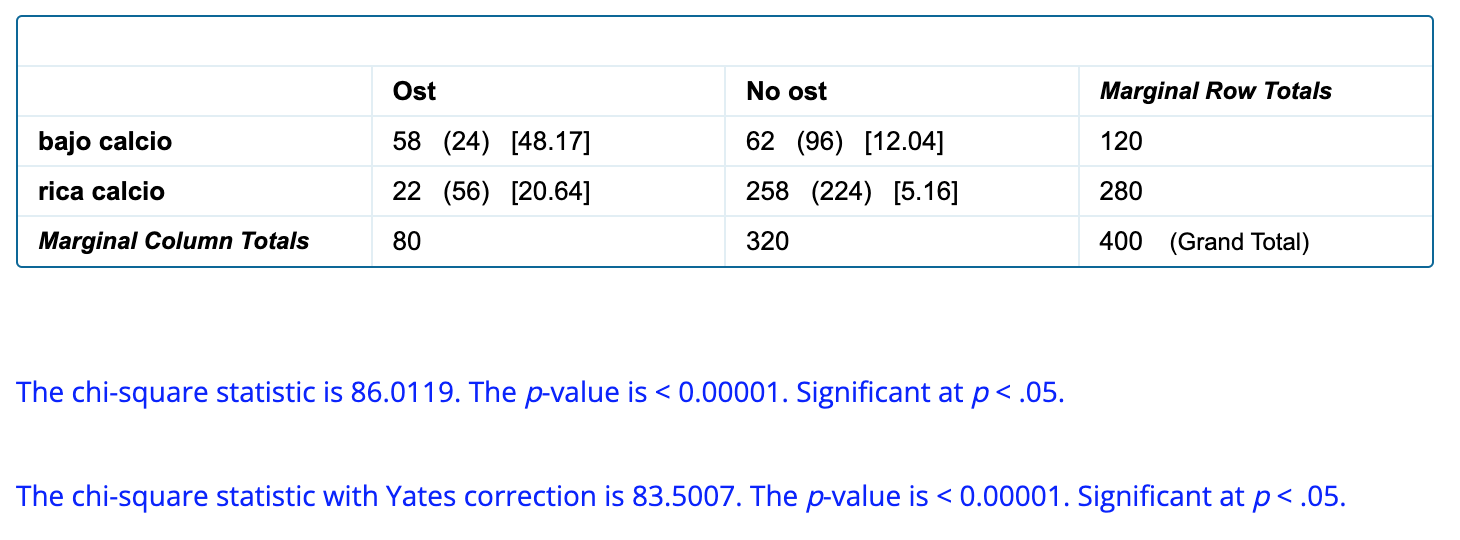
\includegraphics[width=20.28in]{img/5_2}

Ahora la corrección de Yates es 83.5. con valor p \textless{} 0.00001. Se rechaza la la hipótesis de independencia al 5 \% (hay relación significativa)

\textbf{c)} Recoradmos que el \href{https://es.wikipedia.org/wiki/Riesgo_relativo}{Riesgo Relativo} es

\(\dfrac{incidencia ~ acumulada ~ en ~ expuestos}{incidencia ~ acumulada ~ en ~ no ~ expuestos}\)

En nuestro caso:

\(RR = \dfrac{\frac{58}{58+62}}{\frac{22}{22+258}}= 6.15\).

Así, una mujer con antecedentes de dieta baja en calcio tiene 6 veces más posibilidades de padecer osteoporosis que las que no tienen antecedentes de dieta baja en calcio.

\hypertarget{pregunta-test-151}{%
\section{Pregunta test}\label{pregunta-test-151}}

Supongamos que se quiere estudiar la posible asociación entre el hecho de que una gestante fume durante el embarazo y que el niño presente bajo peso al nacer. Para responder a esta pregunta se realiza un estudio de seguimiento sobre una cohorte de 2000 gestantes, a las que se interroga sobre su hábito tabáquico durante la gestación y se determina además el peso del recién nacido. Los resultados de este estudio se muestran en la siguiente tabla:

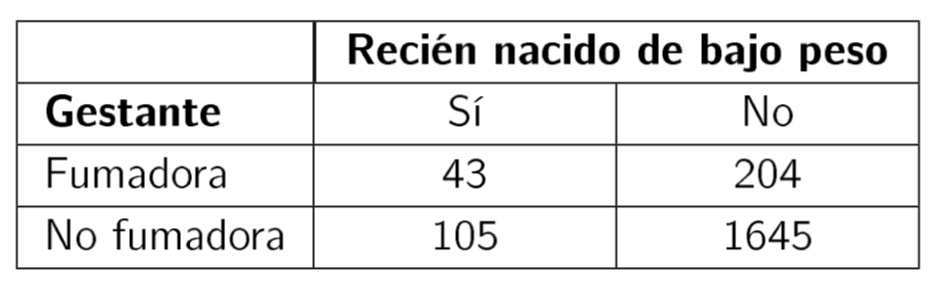
\includegraphics[width=13.08in]{img/5_3}

¿Se puede concluir que, con una confianza del 99\%, existe una relación estadísticamente significativa entre el hecho de que una gestante fume durante el embarazo y que el niño presente bajo peso al nacer?

\begin{enumerate}
\def\labelenumi{\alph{enumi})}
\tightlist
\item
  Sí
\item
  No
\end{enumerate}

Respuesta correcta

\href{https://1fjmanzano.github.io/bioestadistica/me\%CC\%81todos-de-inferencia-estadi\%CC\%81stica.html\#prueba-de-la-chi-cuadrado}{Explicación}

\hypertarget{pregunta-test-152}{%
\section{Pregunta test}\label{pregunta-test-152}}

\hypertarget{problema-16}{%
\section{Problema}\label{problema-16}}

La siguiente tabla muestra la clasificación de 1343 niños según el grado de cumplimiento de su calendario vacunal y el nivel socio-cultural de sus padres. Determina si existe una asociación significativa entre el grado de cumplimiento del calendario vacunal de los niños y el nivel socio- cultural de sus padres.

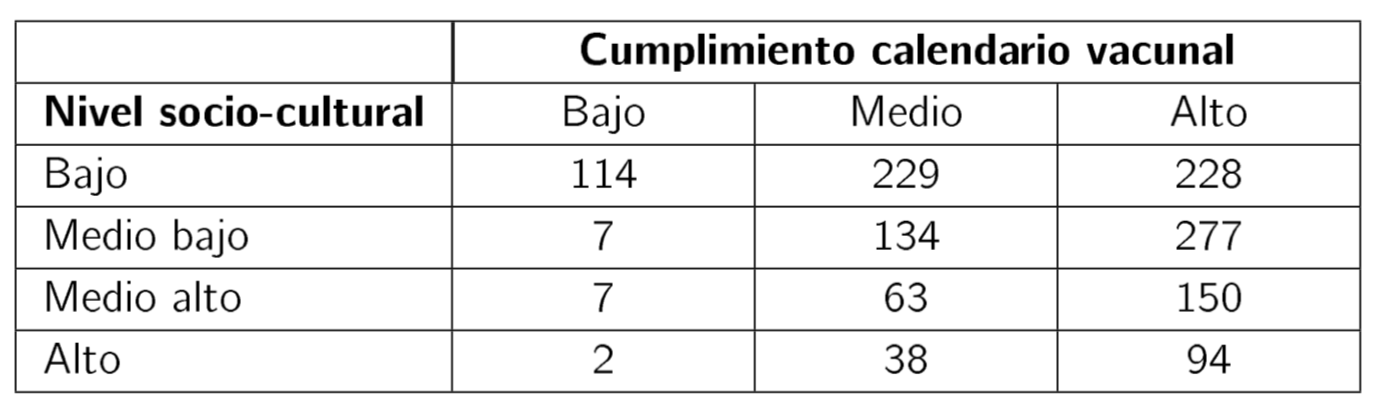
\includegraphics[width=19.11in]{img/5_4}

\hypertarget{soluciuxf3n-12}{%
\subsection{Solución}\label{soluciuxf3n-12}}

En este caso necesitamos la \href{https://www.socscistatistics.com/tests/chisquare2/default2.aspx}{Chi-Square Calculator for 5 x 5 (or less) Contingency Table}. Cumplimentando la tabla y obteniendo los reslutados con una confianza del 95\%:

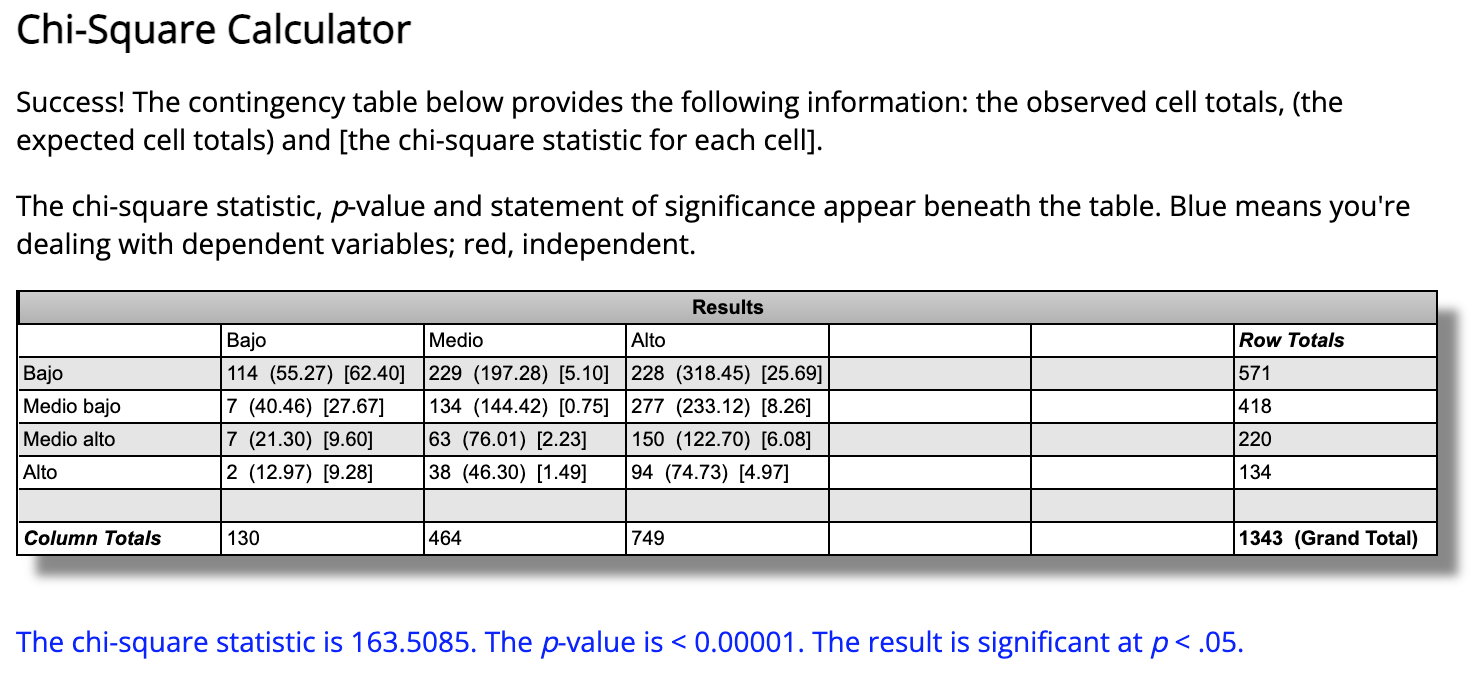
\includegraphics[width=20.44in]{img/5_5}

Así, obtenemos un valor p \textless0.05 por lo que existe una asociación significativa entre el grado de cumplimiento del calendario vacunal de los niños y el nivel socio- cultural de sus padres.

\hypertarget{pregunta-test-153}{%
\section{Pregunta test}\label{pregunta-test-153}}

Para evaluar el efecto de la exposición a asbesto sobre el riesgo de fallecer por cáncer de pulmón, un estudio comparó un grupo de 6.245 trabajadores expuestos a este agente con otro grupo de 7.895 trabajadores sin exposición a este factor. A lo largo de 22 años de seguimiento, en el primer grupo se presentaron 76 defunciones por cáncer en el aparato respiratorio, en tanto que en el grupo no expuesto el número de defunciones por esta causa fue 28. ¿Existe una asociación significativa entre la exposición a asbesto y el riesgo de fallecer por cáncer de pulmón?

\begin{enumerate}
\def\labelenumi{\alph{enumi})}
\tightlist
\item
  Sí
\item
  No
\end{enumerate}

Respuesta correcta

\href{https://1fjmanzano.github.io/bioestadistica/me\%CC\%81todos-de-inferencia-estadi\%CC\%81stica.html\#prueba-de-la-chi-cuadrado}{Explicación}

\hypertarget{pregunta-test-154}{%
\section{Pregunta test}\label{pregunta-test-154}}

En un estudio sobre VIH se pretende determinar si existe asociación signi􏰂cativa entre la edad del paciente y el nivel de linfocitos CD4. Para ello se determina el nivel de linfocitos CD4 (\textless200, 200-500, \textgreater500) en pacientes de 3 grupos de edad. ¿Se puede concluir que existe una relación estadísticamente significativa entre el nivel de linfocitos y la edad del paciente?

\begin{enumerate}
\def\labelenumi{\alph{enumi})}
\tightlist
\item
  Sí
\item
  No
\end{enumerate}

Respuesta correcta

\href{https://1fjmanzano.github.io/bioestadistica/me\%CC\%81todos-de-inferencia-estadi\%CC\%81stica.html\#prueba-de-la-chi-cuadrado}{Explicación}

\hypertarget{pregunta-test-155}{%
\section{Pregunta test}\label{pregunta-test-155}}

Se quiere estudiar la posible asociación entre la presencia de infección postoperatoria (IPO) y la diabetes (DIAB) en una población de operados. En una muestra de 1337 personas de edad \textless{} 65 años y en otra de 892 de edad \(\geq\) 65 años se obtuvieron los siguientes resultados:

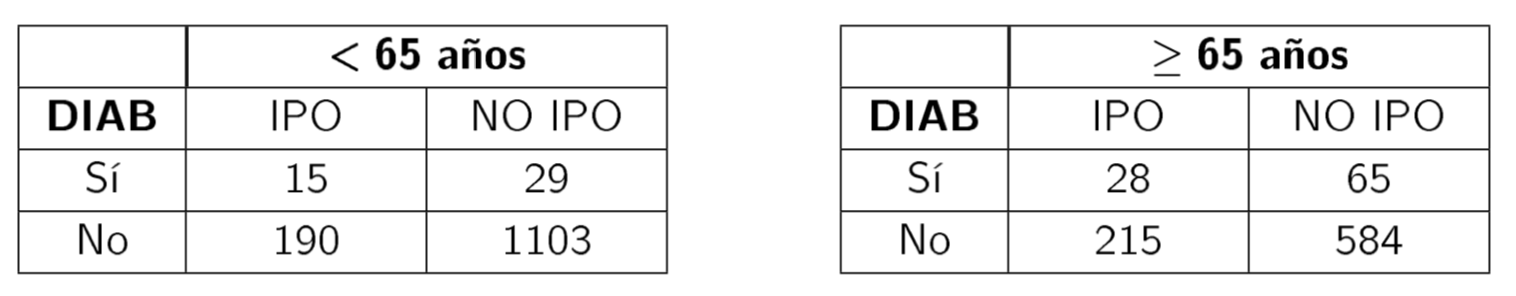
\includegraphics[width=21.06in]{img/5_6}

¿Existe asociación significativa entre IPO y diabetes en cada grupo de edad?

\begin{enumerate}
\def\labelenumi{\alph{enumi})}
\tightlist
\item
  Hay asociación significativa en los dos grupos
\item
  No hay asociación significativa en ningún grupo
\item
  la hay para \textless{} 65 y no para \(\geq\) 65
\item
  no la hay para \textless{} 65 y sí para \(\geq\) 65
\end{enumerate}

Respuesta correcta

\href{https://1fjmanzano.github.io/bioestadistica/me\%CC\%81todos-de-inferencia-estadi\%CC\%81stica.html\#prueba-de-la-chi-cuadrado}{Explicación}

\hypertarget{pregunta-test-156}{%
\section{Pregunta test}\label{pregunta-test-156}}

Se realizó un estudio de seguimiento para detectar la posible asociación entre enfermedades cardiovasculares y el exceso de peso. Se eligieron 1990 hombres con edades entre 55 y 59 años de estatura similar. Tras 5 años de seguimiento se observaron los datos resumidos en la tabla.

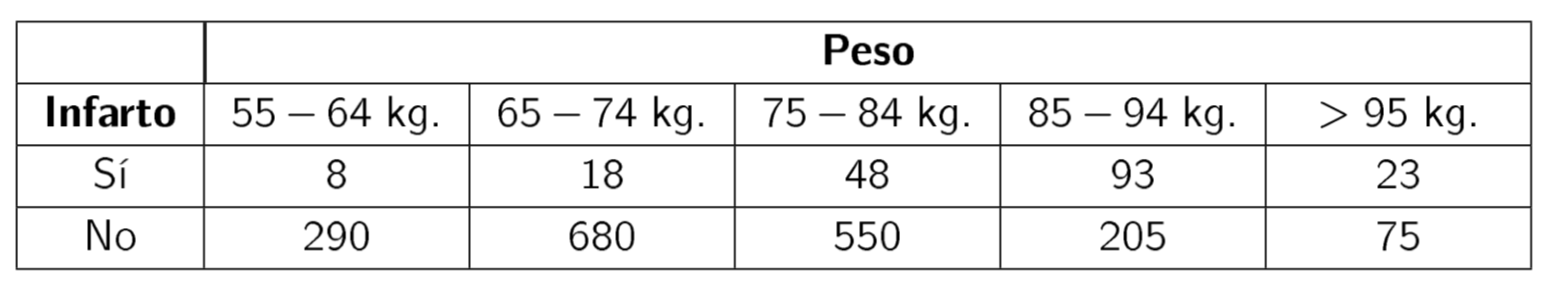
\includegraphics[width=21.47in]{img/5_7}

¿Se puede admitir que el exceso de peso se asocia con el infarto de miocardio?

\begin{enumerate}
\def\labelenumi{\alph{enumi})}
\tightlist
\item
  Sí
\item
  No
\end{enumerate}

Respuesta correcta

\href{https://1fjmanzano.github.io/bioestadistica/me\%CC\%81todos-de-inferencia-estadi\%CC\%81stica.html\#prueba-de-la-chi-cuadrado}{Explicación}

\hypertarget{medidas-de-importancia-cluxednica.}{%
\chapter{Medidas de importancia clínica.}\label{medidas-de-importancia-cluxednica.}}

En este capítulo se resolverán problemas relativos a:

\begin{itemize}
\tightlist
\item
  Diferencias entre Proporción, Tasa, Razón, odds.
\item
  Medidas de asociación en tablas 2x2. Riesgo Relativo. Riesgo Absolutos. Odds-Ratio.
\item
  Indicadores estadísticos básicos para evaluar el desempeño de un procedimiento diagnóstico: Sensibilidad y Especificidad. Probabilidades pre y post prueba.
\end{itemize}

\hypertarget{pregunta-test-157}{%
\section{Pregunta test}\label{pregunta-test-157}}

¿Cómo se denomina la medida de epidemiología que indica la probabilidad de que una enfermedad se desarrolle en un grupo de individuos expuesto a un factor de riesgo comparada con la del grupo no expuesto?

\begin{enumerate}
\def\labelenumi{\alph{enumi})}
\tightlist
\item
  Incidencia acumulada
\item
  Densidad de incidencia
\item
  Fracción atribuible
\item
  Prevalencia
\item
  Riesgo relativo
\end{enumerate}

Respuesta correcta

\href{https://es.wikipedia.org/wiki/Riesgo_relativo}{Explicación}

\hypertarget{pregunta-test-158}{%
\section{Pregunta test}\label{pregunta-test-158}}

En un estudio de casos y controles si se constata asociación estadística mediante la chi- cuadrado clásica ¿Cómo mediremos la magnitud de la asociación?

\begin{enumerate}
\def\labelenumi{\alph{enumi})}
\tightlist
\item
  Riesgo relativo
\item
  Riesgo atribuible
\item
  Fracción de riesgo atribuible
\item
  Odds ratio
\item
  Densidad de incidencia
\end{enumerate}

Respuesta correcta

\href{https://www.elsevier.es/es-revista-educacion-medica-71-articulo-el-odds-ratio-su-interpretacion-S1575181317300360}{Explicación}

\hypertarget{pregunta-test-159}{%
\section{Pregunta test}\label{pregunta-test-159}}

A la capacidad de una prueba diagnóstica para identificar correctamente a los que no padecen la enfermedad se le denomina:

\begin{enumerate}
\def\labelenumi{\alph{enumi})}
\tightlist
\item
  Sensibilidad
\item
  Especificidad
\item
  Valor predictivo positivo
\item
  Valor predictivo negativo
\item
  Razón de probabilidad
\end{enumerate}

Respuesta correcta

\href{https://1fjmanzano.github.io/bioestadistica/relaci\%C3\%B3n-entre-variables-cualitativas.html\#diagno\%CC\%81stico-cli\%CC\%81nico}{Explicacion}

\hypertarget{problema-17}{%
\section{Problema}\label{problema-17}}

Si una prueba diagnóstica tiene una sensibilidad del 75\% y una especificidad del 85\%, calcule la razón de probabilidad positiva.

\hypertarget{soluciuxf3n-13}{%
\subsection{Solución}\label{soluciuxf3n-13}}

La razón de probabilidad positiva, también conocido como \emph{cociente de probabilidad positivo} (CPP) o \emph{likelihood ratio} (LR), nos indica cuánto más probable es tener un positivo en la prueba en un enfermo que en un sano. El uso del LR constituye una herramienta de gran utilidad para la toma de decisiones clínicas frente a la solicitud de algún test diagnóstico, porque son valores inherentes a éste e independientes de la prevalencia de la enfermedad.

Matemáticamente, sería el resultado del cociente:

\(\frac{positivos ~ en ~ enfermos}{positivos ~ en ~ sanos}\)

Sabemos que:

\begin{itemize}
\tightlist
\item
  la proporción de positivos en los enfermos es la Sensibilidad
\item
  la proporción de los positivos en sanos son los Falsos Positivos que serían aquellos sanos que no dan negativo o, lo que es lo mismo, \(1 -\) Especificidad.
\end{itemize}

Entonces, en nuestro problema:

\(CPP= \frac{S}{1-E}= \frac{0.75}{1-0.85}=\frac{0.75}{0.15}=5\)

Así, \textbf{la razón de probabilidad positiva es 5} lo que indica que en esta prueba diagnóstica, un enfermo tiene 5 veces más posibilidades de dar positivo que un sano.

\href{https://www.elsevier.es/es-revista-revista-argentina-radiologia-383-articulo-likelihood-ratio-razon-verosimilitud-definicion-S0048761916301910}{Explicación}

\hypertarget{pregunta-test-160}{%
\section{Pregunta test}\label{pregunta-test-160}}

La proporción de enfermos que han dado un resultado negativo en la prueba diagnóstica dividido entre la proporción de sanos que también han dado negativo en dicha prueba se denomina:

\begin{enumerate}
\def\labelenumi{\alph{enumi})}
\tightlist
\item
  Razón de probabilidad positiva
\item
  Valor predictivo negativo
\item
  Valor predictivo positivo
\item
  Razón de probabilidad negativa
\item
  Especificidad
\end{enumerate}

Respuesta correcta

\href{https://www.redalyc.org/journal/3555/355568264003/html/}{Explicación}

\hypertarget{pregunta-test-161}{%
\section{Pregunta test}\label{pregunta-test-161}}

Si al aplicar una prueba diagnóstica se observa un 10\% de falsos positivos cuál de las siguientes afirmaciones es cierta:

\begin{enumerate}
\def\labelenumi{\alph{enumi})}
\tightlist
\item
  La sensibilidad es el 90\%
\item
  La especificidad es el 90\%
\item
  El valor predictivo positivo es el 90\%
\item
  El cociente de probabilidad positivo es del 90\%
\item
  La sensibilidad es el 10\%
\end{enumerate}

Respuesta correcta

\href{https://1fjmanzano.github.io/bioestadistica/relaci\%C3\%B3n-entre-variables-cualitativas.html\#diagno\%CC\%81stico-cli\%CC\%81nico}{Explicación}

\hypertarget{problema-18}{%
\section{Problema}\label{problema-18}}

Si la probabilidad de tener la enfermedad \(A\) es del 5\%, la de tener la enfermedad \(B\) es del 10\% y la de tener al menos una de las dos es del 13\%, ¿cúal es la probabilidad de tener las dos?

\hypertarget{soluciuxf3n-14}{%
\subsection{Solución}\label{soluciuxf3n-14}}

Éste es un típico problema de Probabilidad con sucesos de Bachillerato que se resuelve muy fácilmente recordando la opraciones con sucesos y los Diagramas de Venn:

\begin{itemize}
\tightlist
\item
  \(A\) = tener la enfermedad \(A\) \(P(A)=0.05\)
\item
  \(B\) = tener la enfermedad \(B\) \(P(B)=0.10\)
\item
  \(A \cap B\) = tener las dos enfermedades
\item
  \(A \cup B\) = tener, al menos, una de las dos enfermedades \(P(A \cup B) = 0.13\)
\end{itemize}

Con un diagrama de Venn:

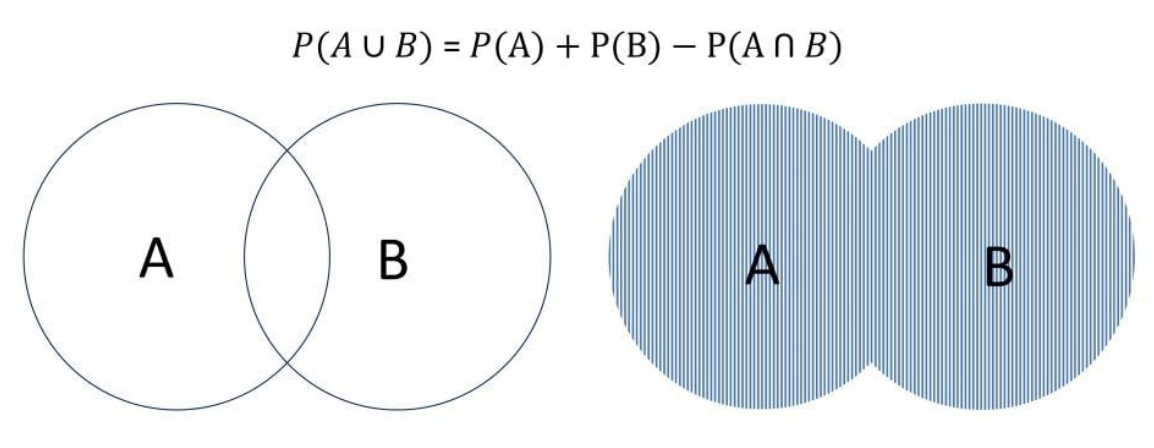
\includegraphics[width=16.03in]{img/7_1}

Así, \(P(A \cup B)=P(A)+P(B)-P(A \cap B) \Rightarrow 0.13=0.05 + 0.10 - P(A \cap B)\)

de donde

\(P(A \cap B)=0.02\)

Entonces, \textbf{la probabilidad de tener las dos enfermedades es del 2\%}.

\hypertarget{pregunta-test-162}{%
\section{Pregunta test}\label{pregunta-test-162}}

En una prueba diagnóstica es importante determinar:

\begin{enumerate}
\def\labelenumi{\alph{enumi})}
\tightlist
\item
  La sensibilidad
\item
  La especificidad
\item
  El valor predictivo positivo
\item
  Todas son ciertas
\end{enumerate}

Respuesta correcta

\href{https://1fjmanzano.github.io/bioestadistica/relaci\%C3\%B3n-entre-variables-cualitativas.html\#diagno\%CC\%81stico-cli\%CC\%81nico}{Explicación}

\hypertarget{pregunta-test-163}{%
\section{Pregunta test}\label{pregunta-test-163}}

Si una prueba diagnóstica se aplica a un grupo de población en el que la prevalencia de la enfermedad es superior a la de la población general aumentará su:

\begin{enumerate}
\def\labelenumi{\alph{enumi})}
\tightlist
\item
  Sensibilidad
\item
  Especificidad
\item
  Valor predictivo positivo
\item
  Razón de probabilidad positivo
\item
  Sensibilidad y especificidad
\end{enumerate}

Respuesta correcta

\href{https://1fjmanzano.github.io/bioestadistica/relaci\%C3\%B3n-entre-variables-cualitativas.html\#diagno\%CC\%81stico-cli\%CC\%81nico}{Explicación}

\hypertarget{problema-19}{%
\section{Problema}\label{problema-19}}

Si una prueba diagnóstica que tiene una sensibilidad del 90\% y una especificidad también del 90\% se aplica a una población de 200 individuos con una prevalencia de enfermedad del 50\% ¿Cuál será el valor predictivo positivo?

\hypertarget{soluciuxf3n-15}{%
\subsection{Solución}\label{soluciuxf3n-15}}

Tenemos que recordar que

\(VPP=\frac{Verdaderos ~ positivos}{Total ~ positivos}=\frac{Verdaderos ~ positivos}{Verdaderos ~ positivos ~ + ~ Falsos ~ positivos}\)

Vamos a hacer una tabla con los datos del problema. Sabemos que:

\begin{longtable}[]{@{}cccc@{}}
\toprule
& Enfermo & Sano &\tabularnewline
\midrule
\endhead
Positivo (+) & & &\tabularnewline
Negativo (-) & & &\tabularnewline
& 100 & 100 & 200\tabularnewline
\bottomrule
\end{longtable}

ya que se aplica a una población de 200 individuos con una prevalencia de enfermedad del 50\% . Ahora:

\begin{itemize}
\tightlist
\item
  la Sensibilidad es la proporción de enfermos que son diagnosticados como positivos (proporción de verdaderos positivos) por lo que:
\end{itemize}

\(0.90 = \hat{P}(+/E) = \frac{verdaderos ~ positivos}{100}\) de donde el numero de verdaderos positivos es 90.

\begin{itemize}
\tightlist
\item
  la Especificidad es la proporción de sanos diagnosticados como negativos (proporción de verdaderos negativos) por lo que:
\end{itemize}

\(0.90 = \hat{P}(-/S) = \frac{verdaderos ~ negativos}{100}\) de donde el numero de verdaderos negativos es 90.

En la tabla:

\begin{longtable}[]{@{}cccc@{}}
\toprule
& Enfermo & Sano &\tabularnewline
\midrule
\endhead
Positivo (+) & 90 & &\tabularnewline
Negativo (-) & & 90 &\tabularnewline
& 100 & 100 & 200\tabularnewline
\bottomrule
\end{longtable}

Terminando de cumplimentar los datos que faltan, tenemos:

\begin{longtable}[]{@{}cccc@{}}
\toprule
& Enfermo & Sano &\tabularnewline
\midrule
\endhead
Positivo (+) & 90 & 10 & 100\tabularnewline
Negativo (-) & 10 & 90 & 100\tabularnewline
& 100 & 100 & 200\tabularnewline
\bottomrule
\end{longtable}

Nos piden el VPP:

\(VPP=\frac{Verdaderos ~ positivos}{Total ~ positivos})\frac{90}{100}=0.90\)

por lo que \textbf{el VPP de la prueba es del 90\%}.

\href{https://1fjmanzano.github.io/bioestadistica/relaci\%C3\%B3n-entre-variables-cualitativas.html\#diagno\%CC\%81stico-cli\%CC\%81nico}{Explicación}

\hypertarget{pregunta-test-164}{%
\section{Pregunta test}\label{pregunta-test-164}}

Cierto tests diagnóstico acierta sobre el 100\% de los individuos enfermos y el 50\% de los sanos. Cierta persona pasa el test con resultado negativo. Entonces:

\begin{enumerate}
\def\labelenumi{\alph{enumi})}
\tightlist
\item
  Esta sana.
\item
  Esta enferma.
\item
  Existe una probabilidad del 50\% de que esté sana.
\item
  Existe una probabilidad del 75\% de que esté sana.
\item
  Existe una probabilidad del 75\% de que esté enferma.
\end{enumerate}

Respuesta correcta

\href{https://1fjmanzano.github.io/bioestadistica/relaci\%C3\%B3n-entre-variables-cualitativas.html\#diagno\%CC\%81stico-cli\%CC\%81nico}{Explicación}

\hypertarget{pregunta-test-165}{%
\section{Pregunta test}\label{pregunta-test-165}}

Si aplicamos una prueba de laboratorio para el diagnóstico de una determinada enfermedad que es 2 veces más frecuente en hombres que en mujeres ¿Cuál de los siguientes parámetros será más elevado en la población femenina que en la masculina?

\begin{enumerate}
\def\labelenumi{\alph{enumi})}
\tightlist
\item
  La prevalencia de la enfermedad
\item
  La sensibilidad de la prueba
\item
  La especificidad de la prueba
\item
  El valor predictivo positivo de la prueba
\item
  El valor predictivo negativo de la prueba
\end{enumerate}

Respuesta correcta

\href{https://1fjmanzano.github.io/bioestadistica/relaci\%C3\%B3n-entre-variables-cualitativas.html\#diagno\%CC\%81stico-cli\%CC\%81nico}{Explicación}

\hypertarget{pregunta-test-166}{%
\section{Pregunta test}\label{pregunta-test-166}}

¿Cómo se calcula la sensibilidad de un test diagnóstico?

\begin{enumerate}
\def\labelenumi{\alph{enumi})}
\tightlist
\item
  Contabilizando el número de tests positivos en una muestra aleatoria de individuos.
\item
  Contabilizando el número de tests negativos en una muestra aleatoria de individuos.
\item
  Contabilizando el número de tests positivos en una muestra aleatoria de enfermos.
\item
  Contabilizando el número de tests negativos en una muestra aleatoria de sanos.
\item
  Ninguna de las anteriores es cierta.
\end{enumerate}

Respuesta correcta

\href{https://1fjmanzano.github.io/bioestadistica/relaci\%C3\%B3n-entre-variables-cualitativas.html\#diagno\%CC\%81stico-cli\%CC\%81nico}{Explicación}

\hypertarget{pregunta-test-167}{%
\section{Pregunta test}\label{pregunta-test-167}}

¿Cuál es la proporción de enfermos sobre el total?

\begin{enumerate}
\def\labelenumi{\alph{enumi})}
\tightlist
\item
  La prevalencia
\item
  La incidencia
\item
  El total de positivos para el test
\item
  El valor predictivo
\item
  El total de las personas estudiadas
\end{enumerate}

Respuesta correcta

\href{https://1fjmanzano.github.io/bioestadistica/relaci\%C3\%B3n-entre-variables-cualitativas.html\#diagno\%CC\%81stico-cli\%CC\%81nico}{Explicación}

\hypertarget{pregunta-test-168}{%
\section{Pregunta test}\label{pregunta-test-168}}

Cierto test diagnóstico acierta sobre el 100\% de los individuos sanos y el 0\% de los individuos enfermos. Elegida una persona al azar:

\begin{enumerate}
\def\labelenumi{\alph{enumi})}
\tightlist
\item
  Hay una probabilidad del 50\% de que esté enferma.
\item
  Hay una probabilidad del 0\% de que esté enferma.
\item
  Hay una probabilidad del 100\% de que esté enferma.
\item
  El test será negativo.
\item
  Ninguna de las anteriores es cierta.
\end{enumerate}

Respuesta correcta

\href{https://1fjmanzano.github.io/bioestadistica/relaci\%C3\%B3n-entre-variables-cualitativas.html\#diagno\%CC\%81stico-cli\%CC\%81nico}{Explicación}

\hypertarget{pregunta-test-169}{%
\section{Pregunta test}\label{pregunta-test-169}}

El parámetro que mide la fuerza de asociación entre la exposición y la enfermedad se denomina:

\begin{enumerate}
\def\labelenumi{\alph{enumi})}
\tightlist
\item
  Factor de riesgo
\item
  Riesgo atribuible
\item
  Factor protector
\item
  Riesgo relativo
\end{enumerate}

Respuesta correcta

\href{https://es.wikipedia.org/wiki/Riesgo_relativo}{Explicación}

\hypertarget{pregunta-test-170}{%
\section{Pregunta test}\label{pregunta-test-170}}

En una población, hay tantos hombres como mujeres, el 20\% son varones y fumadores y el 20\% de las mujeres fuman. Entonces:

\begin{enumerate}
\def\labelenumi{\alph{enumi})}
\tightlist
\item
  Fuman tantos hombres como mujeres.
\item
  Por cada mujer fumadora hay dos hombres fumadores.
\item
  Por cada hombre fumador hay dos mujeres fumadoras.
\item
  Hay un 40\% de fumadores en la población.
\item
  Nada de lo anterior es cierto.
\end{enumerate}

Respuesta correcta

\textbf{Explicación}

Con los datos del problema, tenemos:

\begin{longtable}[]{@{}cccc@{}}
\toprule
& Hombre & Mujer &\tabularnewline
\midrule
\endhead
Fuma (+) & 20 & 10 &\tabularnewline
No fuma (-) & & &\tabularnewline
& 50 & 50 & 100\tabularnewline
\bottomrule
\end{longtable}

(El 20\% de las mujeres fuman, el 20\% del 50\% es 10)

\hypertarget{pregunta-test-171}{%
\section{Pregunta test}\label{pregunta-test-171}}

Para conocer el exceso de riesgo en los individuos expuestos comparando con los no expuestos utilizaremos:

\begin{enumerate}
\def\labelenumi{\alph{enumi})}
\tightlist
\item
  Riesgo relativo
\item
  Diferencia de incidencias
\item
  Odds ratio
\item
  Incidencia acumulada
\item
  Riesgo atribuible
\end{enumerate}

Respuesta correcta

\href{https://es.wikipedia.org/wiki/Riesgo_atribuible}{Explicación}

\hypertarget{pregunta-test-172}{%
\section{Pregunta test}\label{pregunta-test-172}}

Para estudiar la efectividad de un test diagnóstico ante una enfermedad se toma un grupo de 200 personas enfermas y 200 que no la padecen, y se observan los resultados. ¿Qué podemos estimar directamente de ellos?

\begin{enumerate}
\def\labelenumi{\alph{enumi})}
\tightlist
\item
  La sensibilidad y especificidad del test.
\item
  La incidencia de la enfermedad en la población.
\item
  El índice predictivo de verdaderos positivos.
\item
  Son correctas (a) y (c).
\item
  Todo lo anterior.
\end{enumerate}

Respuesta correcta

\href{https://1fjmanzano.github.io/bioestadistica/relaci\%C3\%B3n-entre-variables-cualitativas.html\#diagno\%CC\%81stico-cli\%CC\%81nico}{Explicación}

\hypertarget{pregunta-test-173}{%
\section{Pregunta test}\label{pregunta-test-173}}

¿Cuál de las siguientes medidas utilizaría para cuantificar el imparto potencial de un programa preventivo en la población?

\begin{enumerate}
\def\labelenumi{\alph{enumi})}
\tightlist
\item
  Riesgo relativo
\item
  Odds ratio
\item
  Razón de prevalencia
\item
  Disminución de la prevalencia
\item
  Riesgo atribuible
\end{enumerate}

Respuesta correcta

\href{https://es.wikipedia.org/wiki/Riesgo_atribuible}{Explicación}

\hypertarget{pregunta-test-174}{%
\section{Pregunta test}\label{pregunta-test-174}}

El porcentaje de individuos fumadores o con bronquitis se puede interpretar como una probabilidad:

\begin{enumerate}
\def\labelenumi{\alph{enumi})}
\tightlist
\item
  De un suceso intersección
\item
  Condicionada.
\item
  De un suceso unión.
\item
  A posteriori.
\item
  De un suceso complementario.
\end{enumerate}

Respuesta correcta

\href{https://www.um.es/documents/4874468/11785083/tema-4.pdf/6d391656-5f98-49e4-b8b7-1d8d38767b7e}{Explicación}

\hypertarget{pregunta-test-175}{%
\section{Pregunta test}\label{pregunta-test-175}}

El porcentaje de individuos con bronquitis entre los fumadores se puede interpretar como una probabilidad:

\begin{enumerate}
\def\labelenumi{\alph{enumi})}
\tightlist
\item
  De un suceso intersección
\item
  Condicionada.
\item
  De un suceso unión.
\item
  A posteriori.
\item
  De un suceso complementario.
\end{enumerate}

Respuesta correcta

\href{https://es.wikipedia.org/wiki/Probabilidad_condicionada}{Explicación}

\hypertarget{pregunta-test-176}{%
\section{Pregunta test}\label{pregunta-test-176}}

El porcentaje de individuos con bronquitis que además son fumadores se puede interpretar como una probabilidad:

\begin{enumerate}
\def\labelenumi{\alph{enumi})}
\tightlist
\item
  De un suceso intersección
\item
  Condicionada.
\item
  De un suceso unión.
\item
  A posteriori.
\item
  De un suceso complementario.
\end{enumerate}

Respuesta correcta

\href{https://www.um.es/documents/4874468/11785083/tema-4.pdf/6d391656-5f98-49e4-b8b7-1d8d38767b7e}{Explicación}

\hypertarget{problema-20}{%
\section{Problema}\label{problema-20}}

El 12\% de los individuos de una población padece osteoporosis. EL 25\% de ellos lo sabe. ¿Qué tasa de individuos tiene osteoporosis y lo desconoce?

\hypertarget{soluciuxf3n-16}{%
\subsection{Solución}\label{soluciuxf3n-16}}

Si el 25\% de los que tienen osteoporosis lo sabe, el 75\% de los que tienen osteoporosis lo desconoce. Por lo tanto, la tasa de individuos que tiene osteoporosis y lo desconoce será el 75\% del 12\%, es decir, \(0.75 \cdot 0.12 = 0.09\). Entonces, \textbf{la tasa de individuos que tiene osteoporosis y lo desconoce es del 9\%}.

\hypertarget{pregunta-test-177}{%
\section{Pregunta test}\label{pregunta-test-177}}

¿Cómo se denomina la proporción de enfermos que presentan un resultado positivo de un método diagnostico?

\begin{enumerate}
\def\labelenumi{\alph{enumi})}
\tightlist
\item
  Valor predictivo positivo del método
\item
  Valor predictivo negativo del método
\item
  Especificidad del método
\item
  Razón de probabilidad positiva
\item
  Ninguna de las anteriores
\end{enumerate}

Respuesta correcta

\href{https://1fjmanzano.github.io/bioestadistica/relaci\%C3\%B3n-entre-variables-cualitativas.html\#diagno\%CC\%81stico-cli\%CC\%81nico}{Explicación}

\hypertarget{pregunta-test-178}{%
\section{Pregunta test}\label{pregunta-test-178}}

Una prueba con alta sensibilidad:

\begin{enumerate}
\def\labelenumi{\alph{enumi})}
\tightlist
\item
  Presenta pocos falsos negativos
\item
  Presenta pocos falsos positivos
\item
  Tiene una p \textless{} 0'05
\item
  Necesariamente tiene una especificidad alta
\item
  Presenta muchos falsos positivos
\end{enumerate}

Respuesta correcta

\href{https://1fjmanzano.github.io/bioestadistica/relaci\%C3\%B3n-entre-variables-cualitativas.html\#diagno\%CC\%81stico-cli\%CC\%81nico}{Explicación}

\hypertarget{pregunta-test-179}{%
\section{Pregunta test}\label{pregunta-test-179}}

La probabilidad de que un individuo tomado aleatoriamente en una serie de sujetos de estudio tenga un resultado negativo en las pruebas diagnosticas si realmente no tiene la enfermedad se denomina:

\begin{enumerate}
\def\labelenumi{\alph{enumi})}
\tightlist
\item
  Sensibilidad
\item
  Especificidad
\item
  Proporción de falsos negativos
\item
  Proporción de falsos positivos
\item
  Valor predictivo negativo
\end{enumerate}

Respuesta correcta

\href{https://1fjmanzano.github.io/bioestadistica/relaci\%C3\%B3n-entre-variables-cualitativas.html\#diagno\%CC\%81stico-cli\%CC\%81nico}{Explicación}

\hypertarget{problema-21}{%
\section{Problema}\label{problema-21}}

La osteoporosis afecta 4 veces más a mujeres que a hombres. El 8\% de las mujeres padece osteoporosis en una población donde hay tantos hombres como mujeres. ¿Cuál es la prevalencia de la osteoporosis en la población?

\hypertarget{soluciuxf3n-17}{%
\subsection{Solución}\label{soluciuxf3n-17}}

Hagamos una tabla con los datos:

\begin{longtable}[]{@{}cccc@{}}
\toprule
& Hombres & Mujeres &\tabularnewline
\midrule
\endhead
Osteoporosis (+) & 1 & 4 &\tabularnewline
No Osteoporosis (-) & & &\tabularnewline
& 50 & 50 & 100\tabularnewline
\bottomrule
\end{longtable}

ya que el 50\% son mujeres y el 8\% padece osteoporosis (\(0.08 \cdot 0.50 = 0.04\)) y los hombres que padecen de osteoporosis son la cuarta parte que las mujeres.

Si completamos la tabla:

\begin{longtable}[]{@{}cccc@{}}
\toprule
& Hombres & Mujeres &\tabularnewline
\midrule
\endhead
Osteoporosis (+) & 1 & 4 & 5\tabularnewline
No Osteoporosis (-) & 49 & 46 & 95\tabularnewline
& 50 & 50 & 100\tabularnewline
\bottomrule
\end{longtable}

por lo que \textbf{la prevalencia de la osteoporosis en la población es del 5\%}

\hypertarget{pregunta-test-180}{%
\section{Pregunta test}\label{pregunta-test-180}}

Para conocer los índices (valores) predictivos en un test diagnóstico para una enfermedad que tiene un 1\% de afectados en la población, será necesario conocer:

\begin{enumerate}
\def\labelenumi{\alph{enumi})}
\tightlist
\item
  Sensibilidad y verdaderos positivos
\item
  Prevalencia.
\item
  Verdaderos positivos y prevalencia.
\item
  Especificidad y verdaderos negativos
\item
  Falsos positivos y verdaderos positivos.
\end{enumerate}

Respuesta correcta

\href{https://es.wikipedia.org/wiki/Valores_predictivos}{Explicación}

\hypertarget{pregunta-test-181}{%
\section{Pregunta test}\label{pregunta-test-181}}

Elija la afirmación correcta relativa a pruebas diagnósticas:

\begin{enumerate}
\def\labelenumi{\alph{enumi})}
\tightlist
\item
  La sensibilidad se obtiene usando la noción subjetiva de probabilidad.
\item
  El índice predictivo positivo se obtiene directamente de la noción frecuentista de probabilidad.
\item
  La tasa de verdaderos positivos se obtiene directamente de la noción frecuentista de probabilidad.
\item
  La prevalencia de la enfermedad se obtiene a partir del teorema de Bayes.
\item
  nada de lo anterior es cierto.
\end{enumerate}

Respuesta correcta

\href{https://1fjmanzano.github.io/bioestadistica/relaci\%C3\%B3n-entre-variables-cualitativas.html\#diagno\%CC\%81stico-cli\%CC\%81nico}{Explicación}

\hypertarget{pregunta-test-182}{%
\section{Pregunta test}\label{pregunta-test-182}}

El 2\% de la población padece diabetes. Si de ellos, el 30\% no está diagnósticado, esta cantidad puede entenderse como una probabilidad\ldots{}

\begin{enumerate}
\def\labelenumi{\alph{enumi})}
\tightlist
\item
  De un suceso intersección
\item
  Condicionada.
\item
  De un suceso unión.
\item
  A posteriori.
\item
  De un suceso complementario.
\end{enumerate}

Respuesta correcta

\href{https://es.wikipedia.org/wiki/Probabilidad_condicionada}{Explicación}

\hypertarget{problema-22}{%
\section{Problema}\label{problema-22}}

En una población, el 5\% son enfermos diagnosticados de una enfermedad, la cual padece el 10\% de la población. Calcular la probabilidad de estar diagnósticado para un individuo enfermo.

\hypertarget{soluciuxf3n-18}{%
\subsection{Solución}\label{soluciuxf3n-18}}

Éste es un problema de probabilidad condicionada. \href{https://es.wikipedia.org/wiki/Probabilidad_condicionada}{Recordamos}:

\(P(A/B)=\frac{P(A \cap B)}{P(B)}\)

En nuestro caso:

\begin{itemize}
\tightlist
\item
  \(E\) = estar enfermo \(P(E)=0.10\)
\item
  \(D\) = estar diagnosticado
\item
  \(E \cap D\) = estar enfermo y diagnosticado \(P(E \cap D) = 0.05\)
\end{itemize}

Se pide calcular la probabilidad de estar diagnósticado para un individuo enfermo, es decir, \(P(D/E)\). Entonces:

\(P(D/E)=\frac{P(D \cap E)}{P(E)}= \frac{0.05}{0.10}=0.50\)

Así, \textbf{la probabilidad de estar diagnósticado para un individuo enfermo es del 50\%}.

\hypertarget{pregunta-test-183}{%
\section{Pregunta test}\label{pregunta-test-183}}

Una prueba diagnóstica de cierta enfermedad, tiene una tasa de aciertos del 90\% tanto sobre enfermos como sanos. La incidencia de la enfermedad en la población es del 50\%. Si se pasa el test a una persona y sale positivo, la probabilidad de que realmente esté enferma es:

\begin{enumerate}
\def\labelenumi{\alph{enumi})}
\tightlist
\item
  45\%
\item
  50\%
\item
  75\%
\item
  90\%
\item
  100\%
\end{enumerate}

Respuesta correcta

\href{https://1fjmanzano.github.io/bioestadistica/relaci\%C3\%B3n-entre-variables-cualitativas.html\#diagno\%CC\%81stico-cli\%CC\%81nico}{Explicación}

\hypertarget{problema-23}{%
\section{Problema}\label{problema-23}}

Una enfermedad tiene una incidencia del 50\% en la población. Un test para detectarla posee una tasa de verdaderos positivos del 80\%, y de falsos positivos del 20\%. Si un individuo resulta ser positivo, calcular la probabilidad de que esté enfermo.

\hypertarget{soluciuxf3n-19}{%
\subsection{Solución}\label{soluciuxf3n-19}}

En este caso, vamos a hacer una tabla de contingencia con los datos para 200 individuos:

\begin{longtable}[]{@{}cccc@{}}
\toprule
& Enfermo (E) & Sano (S) &\tabularnewline
\midrule
\endhead
Positivo (+) & 80 & 20 &\tabularnewline
Negativo (-) & & &\tabularnewline
& 100 & 100 & 200\tabularnewline
\bottomrule
\end{longtable}

Si completamos la tabla:

\begin{longtable}[]{@{}cccc@{}}
\toprule
& Enfermo (E) & Sano (S) &\tabularnewline
\midrule
\endhead
Positivo (+) & 80 & 20 & 100\tabularnewline
Negativo (-) & 20 & 80 & 100\tabularnewline
& 100 & 100 & 200\tabularnewline
\bottomrule
\end{longtable}

Se pide que, si un individuo resulta ser positivo, calcular la probabilidad de que esté enfermo, es decir \(P(E/+)= \frac{80}{100}=0.80\).

Entonces \textbf{Si un individuo resulta ser positivo, la probabilidad de que esté enfermo es del 80\%}.

\hypertarget{pregunta-test-184}{%
\section{Pregunta test}\label{pregunta-test-184}}

En una población el 30\% son hombres de los cuales son deportistas el 20\%, frente al 25\% de las mujeres. Escogida una persona al azar es deportista. La probabilidad de que sea mujer es (aproximadamente):

\begin{enumerate}
\def\labelenumi{\alph{enumi})}
\tightlist
\item
  \(0,235\)
\item
  \(0,60\)
\item
  \(0,74\)
\item
  \(0,25\)
\item
  No puede calcularse con esos datos.
\end{enumerate}

Respuesta correcta

\hypertarget{referencias}{%
\chapter{Referencias}\label{referencias}}

\begin{itemize}
\item
  \href{https://www.bioestadistica.uma.es/baron/apuntes/}{Apuntes y vídeos de Bioestadística, Francisco Javier Barón López}
\item
  \href{https://personal.us.es/pmr/index.php/docencia/cursos-anteriores/88-2011-2012/94-matematica-aplicada-y-estadistica-grado-en-farmacia-2011-2012}{Matemática Aplicada y Estadística (Grado en Farmacia) 2011/2012}
\item
  \href{http://eduardobuesa.es}{Dr.~Eduardo Buesa. Jefe emérito del Servicio de Pediatría. Hospital General de Castellón}
\item
  \href{https://aprendeconalf.es/docencia/estadistica/examenes/}{Exámenes de Estadística}
\item
  \href{https://epidemiologiamolecular.com/investigacion-epidemiologica/test-de-bioestadistica/}{EMEI. Epidemiología Molecular de Enfermedades Infecciosas. Test de Bioestadística}
\end{itemize}

  \bibliography{book.bib,packages.bib}

\end{document}
